% ======= NỘI DUNG =======
\chapter{Phân tích và Thiết kế}
\label{chap:PhanTichVaThietKe}

\section{Phân tích}
\label{sec:PhanTich}

% ======= NỘI DUNG PHẦN PHÂN TÍCH USE CASE =======
\subsection{Mô hình hóa tương tác (Biểu đồ Usecase)}
\label{subsec:BieuDoCaSuDung}
\begin{figure}[htbp]
 \centering
 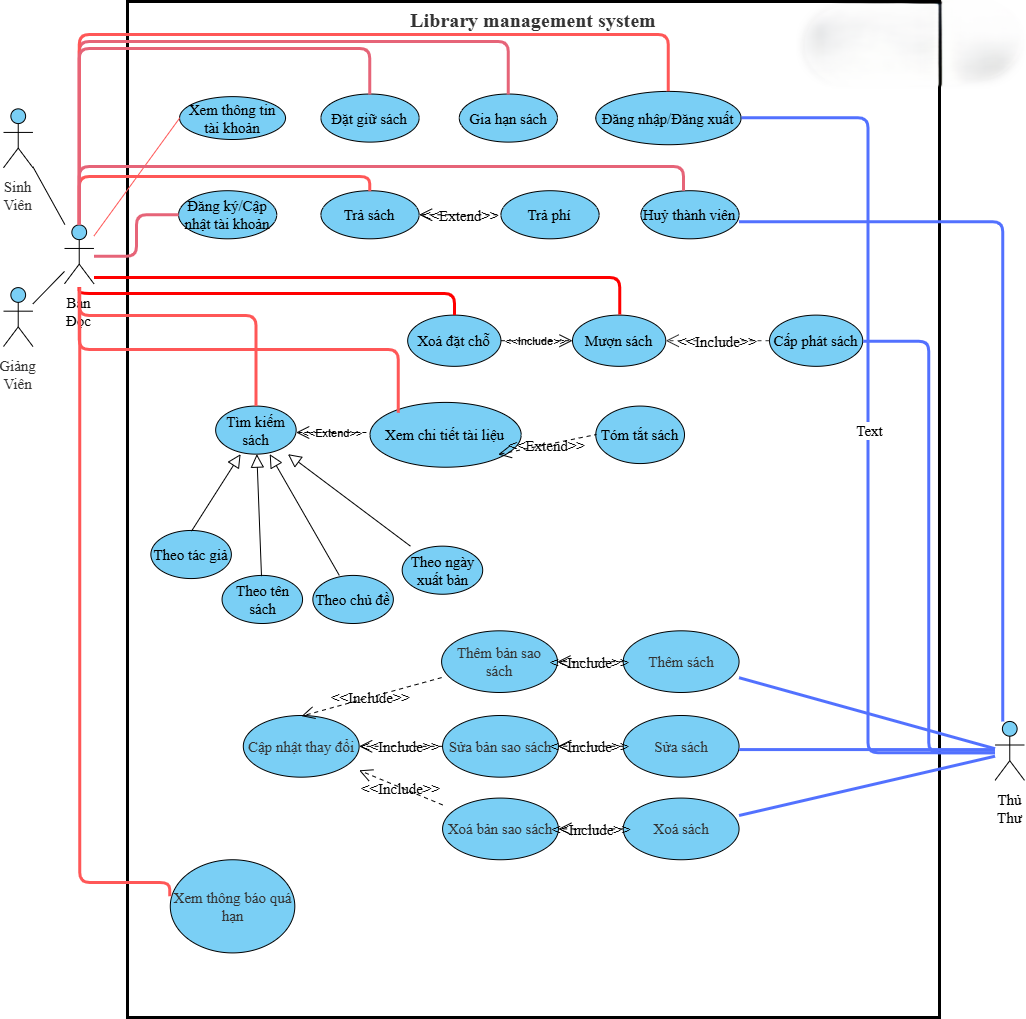
\includegraphics[width=0.95\linewidth]{images/V.Analysis_and_Design/usecase/usecase.png}
 \caption{Biểu đồ Usecase tổng quát của Hệ thống Quản lý Thư viện}
 \label{fig:bieudo_ca_sudung}
\end{figure}

\subsubsection{Đặc tả chi tiết các Use Case chính}
\begin{table}[H]
\centering
\caption{Bảng đặc tả Use Case UC-01: Tìm kiếm sách}
\label{tab:dt_tim_kiem_sach}
\begin{tabular}{|>{\raggedright\arraybackslash}p{0.25\linewidth}|>{\raggedright\arraybackslash}p{0.65\linewidth}|}
\hline
\textbf{Thuộc tính} & \textbf{Mô tả chi tiết} \\
\hline
\textbf{Tên Use Case} & Tìm kiếm sách \\
\hline
\textbf{Mã số} & UC-01 \\
\hline
\textbf{Tác nhân} & Bạn đọc, Thủ thư \\
\hline
\textbf{Mô tả ngắn gọn} & Cho phép người dùng tìm kiếm các tài liệu trong thư viện dựa trên các tiêu chí khác nhau như tiêu đề, tác giả, chủ đề. \\
\hline
\textbf{Tiền điều kiện} & Người dùng đã truy cập vào giao diện tìm kiếm của hệ thống. \\
\hline
\textbf{Hậu điều kiện} & \textbf{Thành công:} Hệ thống hiển thị danh sách các tài liệu phù hợp với tiêu chí tìm kiếm. \newline \textbf{Thất bại:} Hệ thống hiển thị thông báo "Không tìm thấy kết quả phù hợp". \\
\hline
\textbf{Luồng chính} &
1. Người dùng nhập từ khóa vào ô tìm kiếm. \newline
2. Người dùng có thể chọn bộ lọc (tác giả, chủ đề,...). \newline
3. Người dùng nhấn nút "Tìm kiếm". \newline
4. Hệ thống truy vấn cơ sở dữ liệu và trả về danh sách kết quả. \newline
5. Hệ thống hiển thị danh sách kết quả cho người dùng. Use case kết thúc. \\
\hline
\textbf{Luồng thay thế} &
\textbf{4a. Không có kết quả phù hợp:} \newline
\hspace{1em} 1. Hệ thống hiển thị thông báo "Không tìm thấy kết quả phù hợp". Use case kết thúc. \\
\hline
\end{tabular}
\end{table}

\begin{table}[H]
\centering
\caption{Bảng đặc tả Use Case UC-02: Đăng ký tài khoản}
\label{tab:dt_dang_ky}
\begin{tabular}{|>{\raggedright\arraybackslash}p{0.25\linewidth}|>{\raggedright\arraybackslash}p{0.65\linewidth}|}
\hline
\textbf{Thuộc tính} & \textbf{Mô tả chi tiết} \\
\hline
\textbf{Tên Use Case} & Đăng ký tài khoản \\
\hline
\textbf{Mã số} & UC-02 \\
\hline
\textbf{Tác nhân} & Bạn đọc (người dùng mới) \\
\hline
\textbf{Mô tả ngắn gọn} & Cho phép người dùng mới tạo một tài khoản thành viên để sử dụng các dịch vụ của thư viện. \\
\hline
\textbf{Tiền điều kiện} & Người dùng đang ở trang đăng ký của hệ thống. \\
\hline
\textbf{Hậu điều kiện} & \textbf{Thành công:} Một tài khoản mới được tạo trong hệ thống và người dùng được đăng nhập tự động. \newline \textbf{Thất bại:} Tài khoản không được tạo, hệ thống hiển thị thông báo lỗi. \\
\hline
\textbf{Luồng chính} &
1. Người dùng nhập thông tin cá nhân vào biểu mẫu đăng ký (Họ tên, email, mật khẩu,...). \newline
2. Người dùng nhấn nút "Đăng ký". \newline
3. Hệ thống kiểm tra tính hợp lệ của thông tin (định dạng email, mật khẩu đủ mạnh). \newline
4. Hệ thống kiểm tra xem email đã tồn tại trong cơ sở dữ liệu chưa. \newline
5. Hệ thống tạo tài khoản mới và lưu thông tin vào cơ sở dữ liệu. \newline
6. Hệ thống tự động đăng nhập cho người dùng và chuyển hướng đến trang cá nhân. Use case kết thúc. \\
\hline
\textbf{Luồng thay thế} &
\textbf{3a. Thông tin không hợp lệ:} \newline
\hspace{1em} 1. Hệ thống hiển thị thông báo lỗi tương ứng với từng trường thông tin. Người dùng được yêu cầu nhập lại. \newline
\textbf{4a. Email đã tồn tại:} \newline
\hspace{1em} 1. Hệ thống hiển thị thông báo "Email này đã được sử dụng". Người dùng được yêu cầu sử dụng email khác. \\
\hline
\end{tabular}
\end{table}

\begin{table}[H]
\centering
\caption{Bảng đặc tả Use Case UC-08: Mượn sách}
\label{tab:dt_muon_sach}
\begin{tabular}{|>{\raggedright\arraybackslash}p{0.25\linewidth}|>{\raggedright\arraybackslash}p{0.65\linewidth}|}
\hline
\textbf{Thuộc tính} & \textbf{Mô tả chi tiết} \\
\hline
\textbf{Tên Use Case} & Mượn sách \\
\hline
\textbf{Mã số} & UC-08 \\
\hline
\textbf{Tác nhân} & Thủ thư \\
\hline
\textbf{Mô tả ngắn gọn} & Thủ thư ghi nhận thông tin một Bạn đọc mượn một bản sao sách cụ thể, cập nhật trạng thái của sách và hồ sơ của bạn đọc. \\
\hline
\textbf{Tiền điều kiện} &
1. Thủ thư đã đăng nhập vào hệ thống. \newline
2. Bạn đọc có tài khoản đang ở trạng thái hoạt động. \newline
3. Bản sao sách có trạng thái "Sẵn có". \\
\hline
\textbf{Hậu điều kiện} &
\textbf{Thành công:} Một bản ghi mượn sách mới được tạo; Trạng thái của bản sao sách được cập nhật thành "Đã cho mượn"; Số lượng sách đang mượn của bạn đọc được cập nhật. \newline
\textbf{Thất bại:} Trạng thái hệ thống không thay đổi. \\
\hline
\textbf{Luồng chính} &
1. Thủ thư khởi tạo chức năng "Mượn sách". \newline
2. Hệ thống yêu cầu nhập/quét mã vạch phiếu mượn của bạn đọc. \newline
3. Thủ thư nhập/quét mã phiếu mượn của bạn đọc. \newline
4. Hệ thống xác thực và hiển thị thông tin tóm tắt của Bạn đọc. \newline
5. Hệ thống yêu cầu nhập/quét mã vạch của Bản sao sách. \newline
6. Thủ thư nhập/quét mã Bản sao sách. \newline
7. Hệ thống xác thực và kiểm tra trạng thái "Sẵn có" của sách. \newline
8. Hệ thống kiểm tra các quy tắc nghiệp vụ (xem Luồng thay thế). \newline
9. Use case này \textbf{bao gồm} use case "Xóa đặt chỗ" (nếu bạn đọc có đặt trước cuốn sách này). \newline
10. Use case này \textbf{bao gồm} use case "Cấp phát sách". \newline
11. Hệ thống xác nhận giao dịch thành công, hiển thị ngày hết hạn. Use case kết thúc. \\
\hline
\textbf{Luồng thay thế} &
\textbf{4a. Bạn đọc không tồn tại hoặc tài khoản bị khóa:} \newline
\hspace{1em} 1. Hệ thống hiển thị thông báo lỗi. Use case kết thúc. \newline
\textbf{7a. Bản sao sách không tồn tại hoặc không ở trạng thái "Sẵn có":} \newline
\hspace{1em} 1. Hệ thống hiển thị thông báo lỗi. Use case kết thúc. \newline
\textbf{8a. Bạn đọc đã mượn đủ số lượng sách tối đa cho phép:} \newline
\hspace{1em} 1. Hệ thống hiển thị thông báo lỗi. Use case kết thúc. \\
\hline
\end{tabular}
\end{table}

\begin{table}[H]
\centering
\caption{Bảng đặc tả Use Case UC-09: Trả sách}
\label{tab:dt_tra_sach}
\begin{tabular}{|>{\raggedright\arraybackslash}p{0.25\linewidth}|>{\raggedright\arraybackslash}p{0.65\linewidth}|}
\hline
\textbf{Thuộc tính} & \textbf{Mô tả chi tiết} \\
\hline
\textbf{Tên Use Case} & Trả sách \\
\hline
\textbf{Mã số} & UC-09 \\
\hline
\textbf{Tác nhân} & Bạn đọc, Thủ thư \\
\hline
\textbf{Mô tả ngắn gọn} & Ghi nhận việc Bạn đọc trả lại một cuốn sách đã mượn. Hệ thống cập nhật trạng thái sách và kiểm tra các khoản phí phạt (nếu có). \\
\hline
\textbf{Tiền điều kiện} & Sách đang ở trạng thái "Đã cho mượn" bởi một bạn đọc cụ thể. \\
\hline
\textbf{Hậu điều kiện} & \textbf{Thành công:} Trạng thái bản sao sách được cập nhật thành "Sẵn có". Bản ghi mượn sách được đóng lại. \newline \textbf{Thất bại:} Trạng thái hệ thống không thay đổi. \\
\hline
\textbf{Luồng chính} &
1. Thủ thư khởi tạo chức năng "Trả sách". \newline
2. Hệ thống yêu cầu nhập/quét mã vạch của bản sao sách. \newline
3. Người dùng nhập/quét mã vạch sách. \newline
4. Hệ thống tìm bản ghi mượn sách tương ứng và kiểm tra ngày trả so với ngày hết hạn. \newline
5. Hệ thống cập nhật trạng thái bản sao sách thành "Sẵn có". \newline
6. Hệ thống đóng bản ghi mượn sách. Use case kết thúc. \\
\hline
\textbf{Luồng thay thế} &
\textbf{4a. Sách bị trả muộn (extend):} \newline
\hspace{1em} 1. Nếu ngày trả > ngày hết hạn, hệ thống sẽ kích hoạt use case "Trả phí". \\
\hline
\end{tabular}
\end{table}


\subsection{Mô hình hoá quy trình nghiệp vụ (Activity diagram)}
\label{subsec:ActivityDiagram}

% + Đăng ký tài khoản
\begin{figure}[htbp]
 \centering
 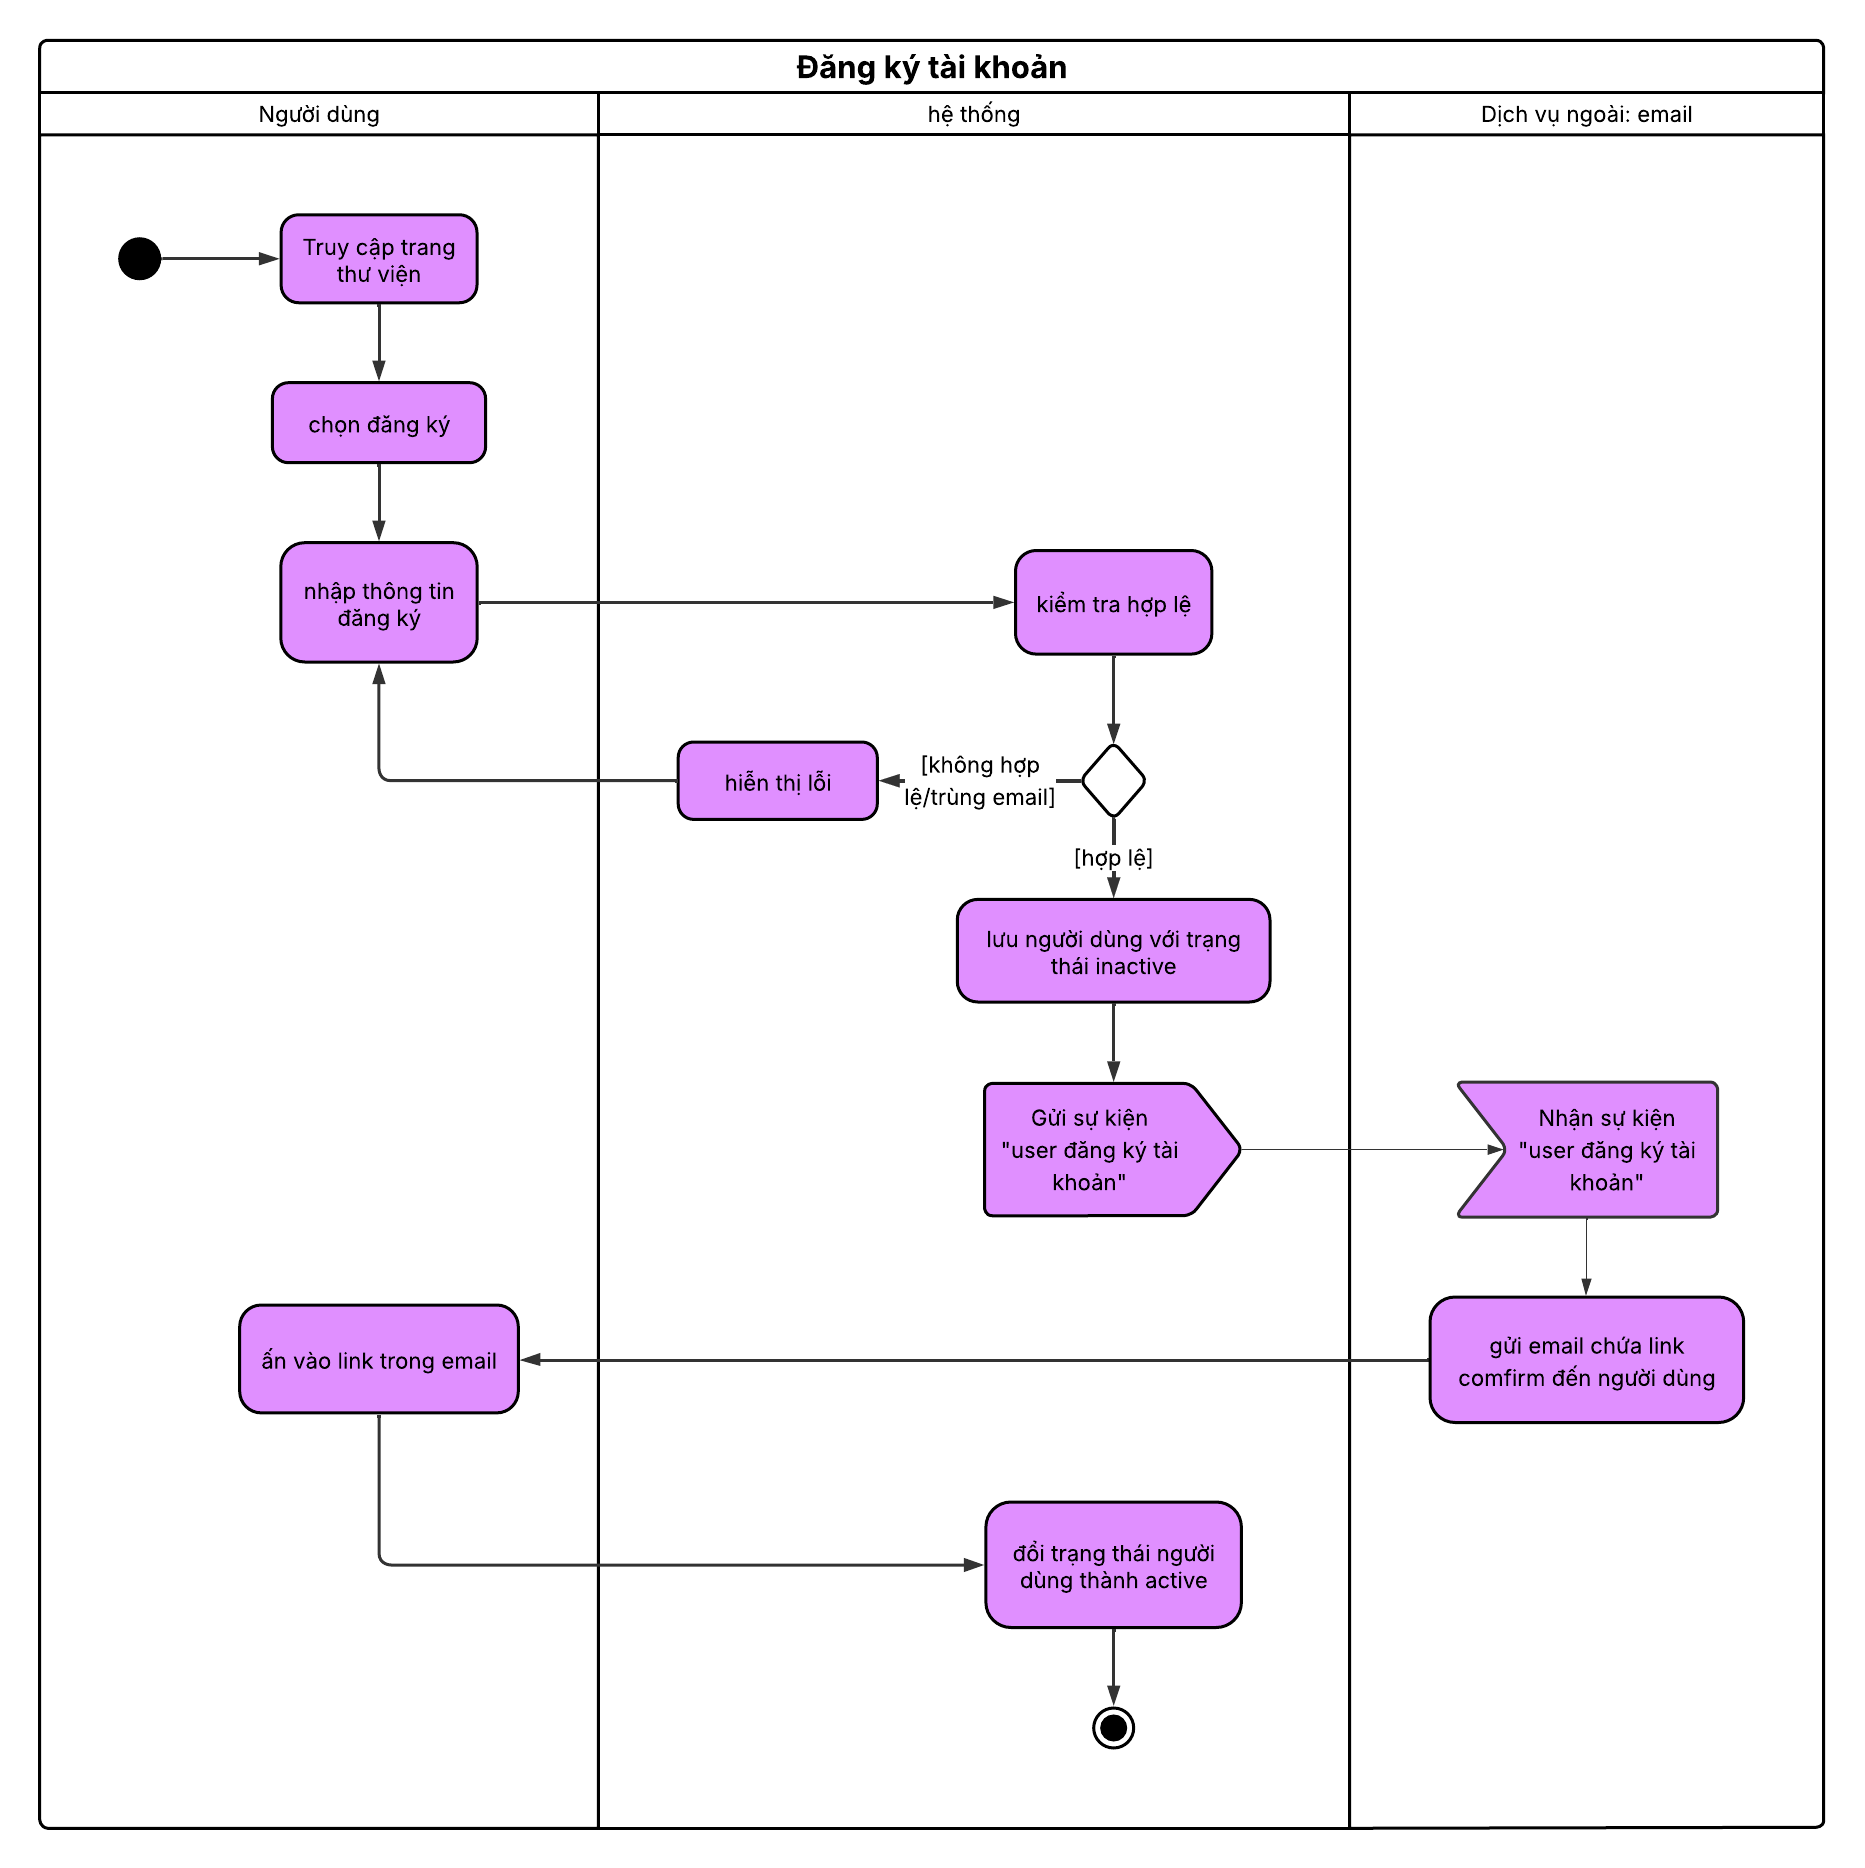
\includegraphics[width=1\linewidth]{images/V.Analysis_and_Design/activity_diagram/sign_up.png}
 \caption{Đăng ký tài khoản — Activity Diagram}
 \label{fig:signup}
\end{figure}

% + Đăng nhập tài khoản
\begin{figure}[htbp]
 \centering
 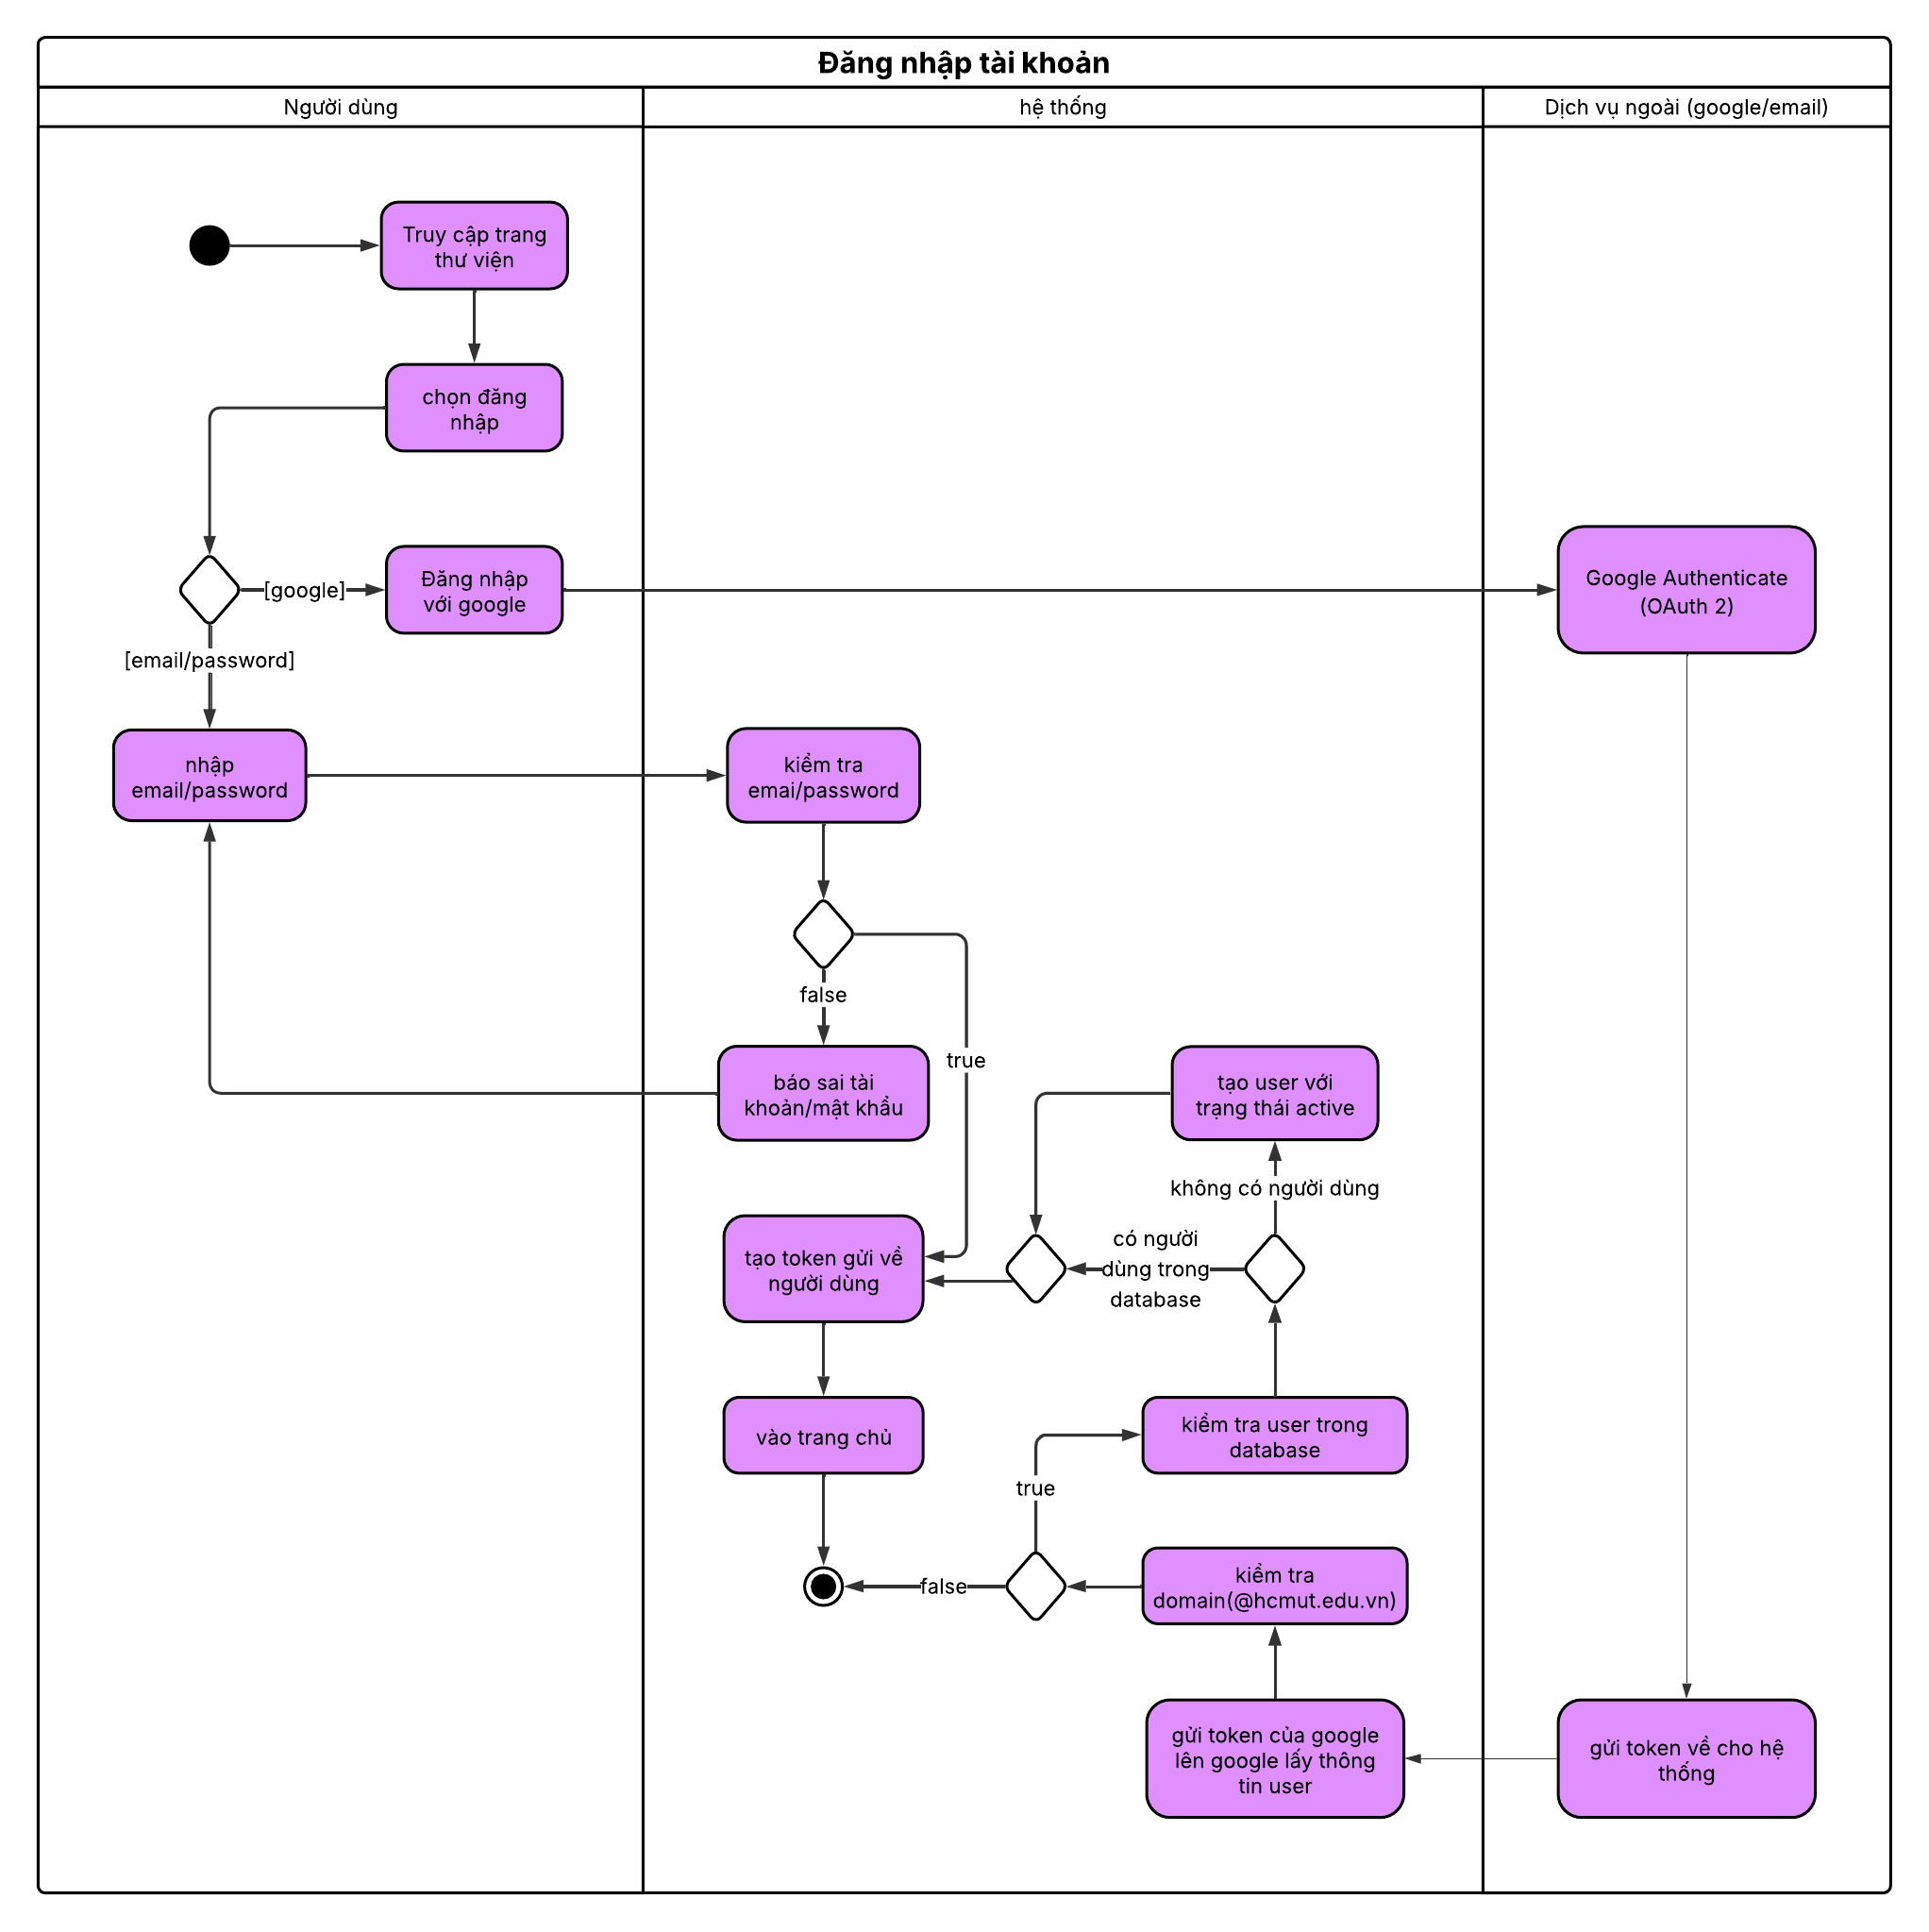
\includegraphics[width=1\linewidth]{images/V.Analysis_and_Design/activity_diagram/login.png}
 \caption{Đăng nhập tài khoản — Activity Diagram}
 \label{fig:signin}
\end{figure}

% + Tìm kiếm sách:
\begin{figure}[htbp]
 \centering
 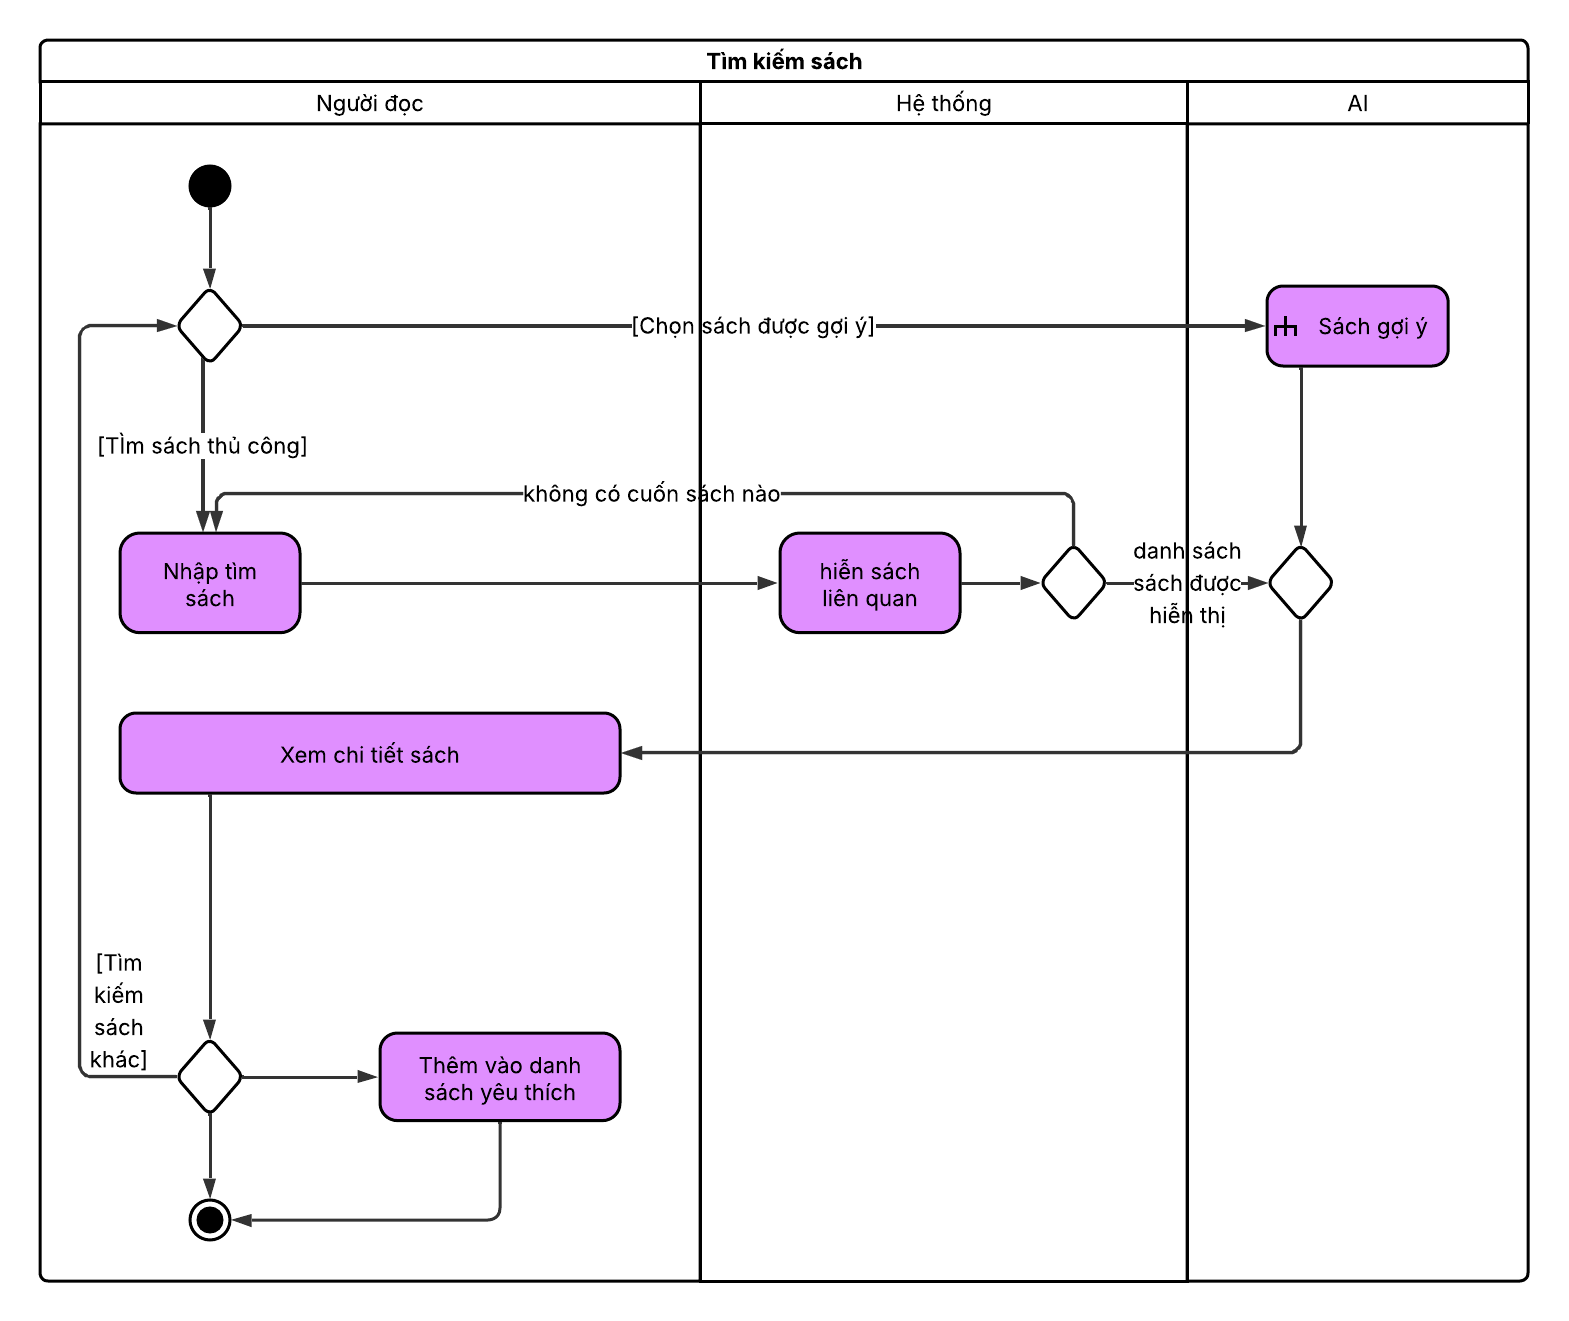
\includegraphics[width=\linewidth]{images/V.Analysis_and_Design/activity_diagram/search_book.png}
 \caption{Tìm kiếm sách — Activity Diagram}
 \label{fig:search-book}
\end{figure}

% + Gợi ý sách:
\begin{figure}[htbp]
 \centering
 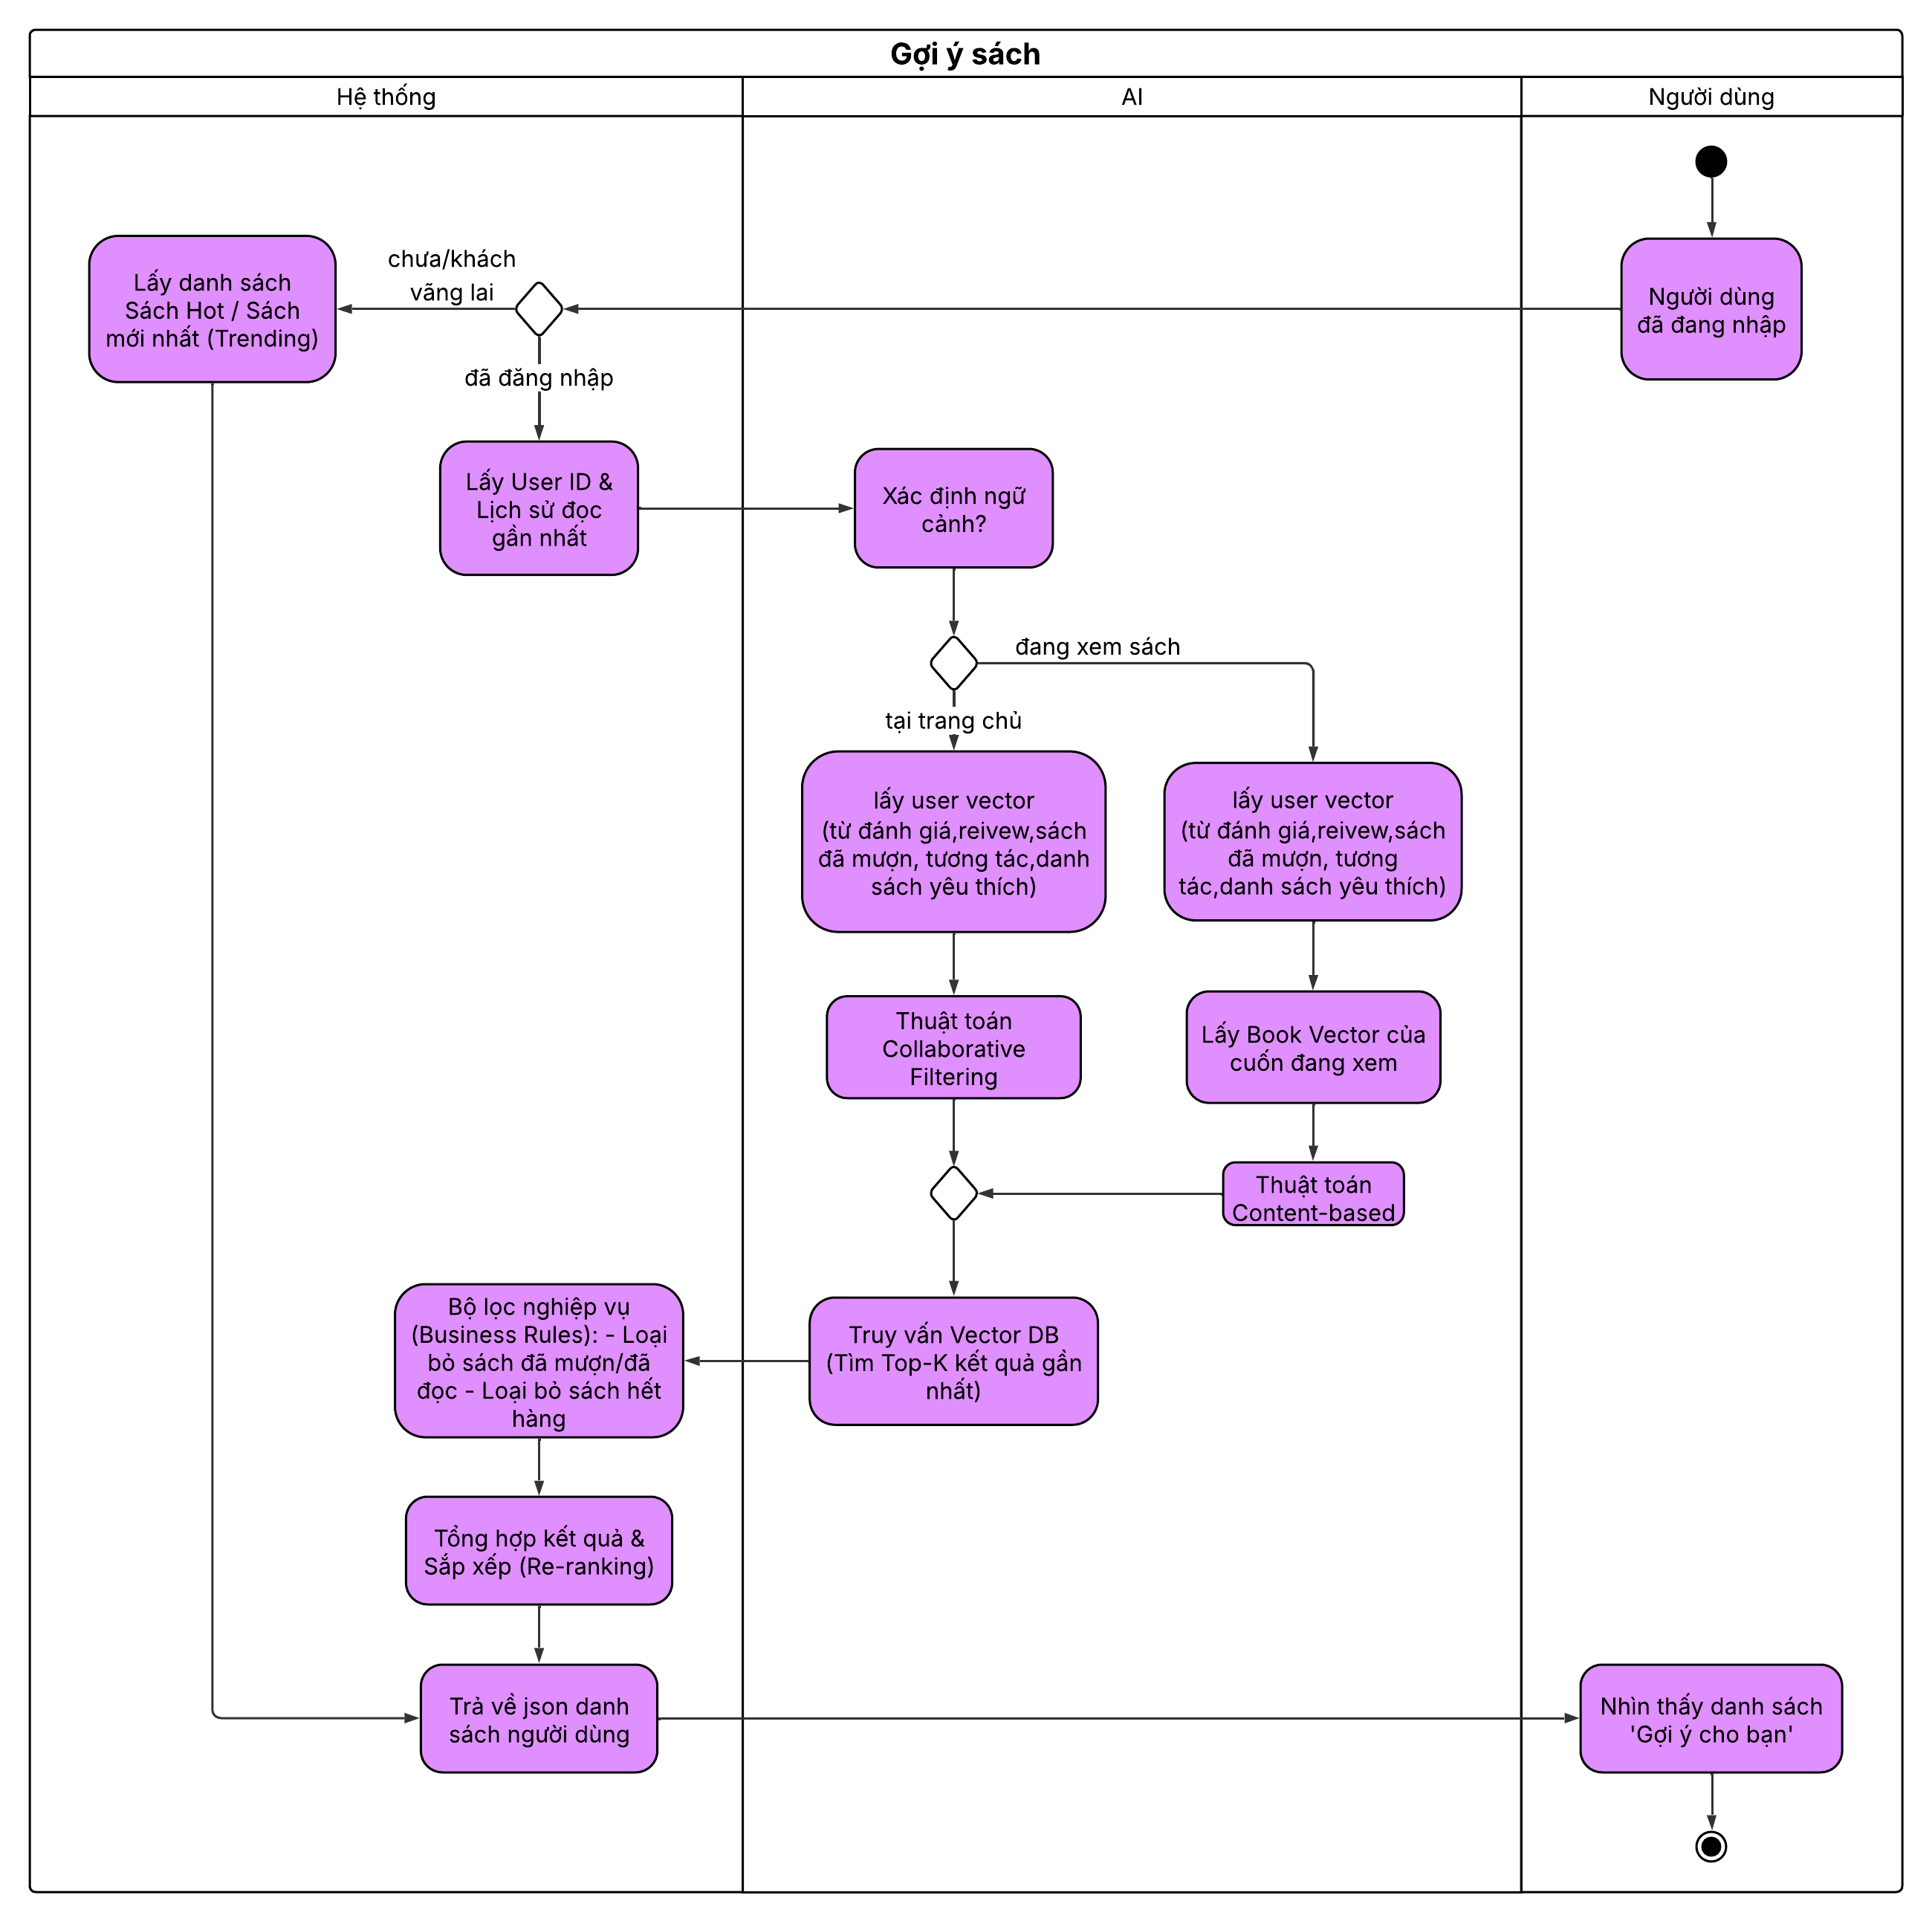
\includegraphics[width=\linewidth]{images/V.Analysis_and_Design/activity_diagram/suggest_book.png}
 \caption{Gợi ý sách — Activity Diagram}
 \label{fig:suggestion}
\end{figure}

\begin{figure}[htbp]
 \centering
 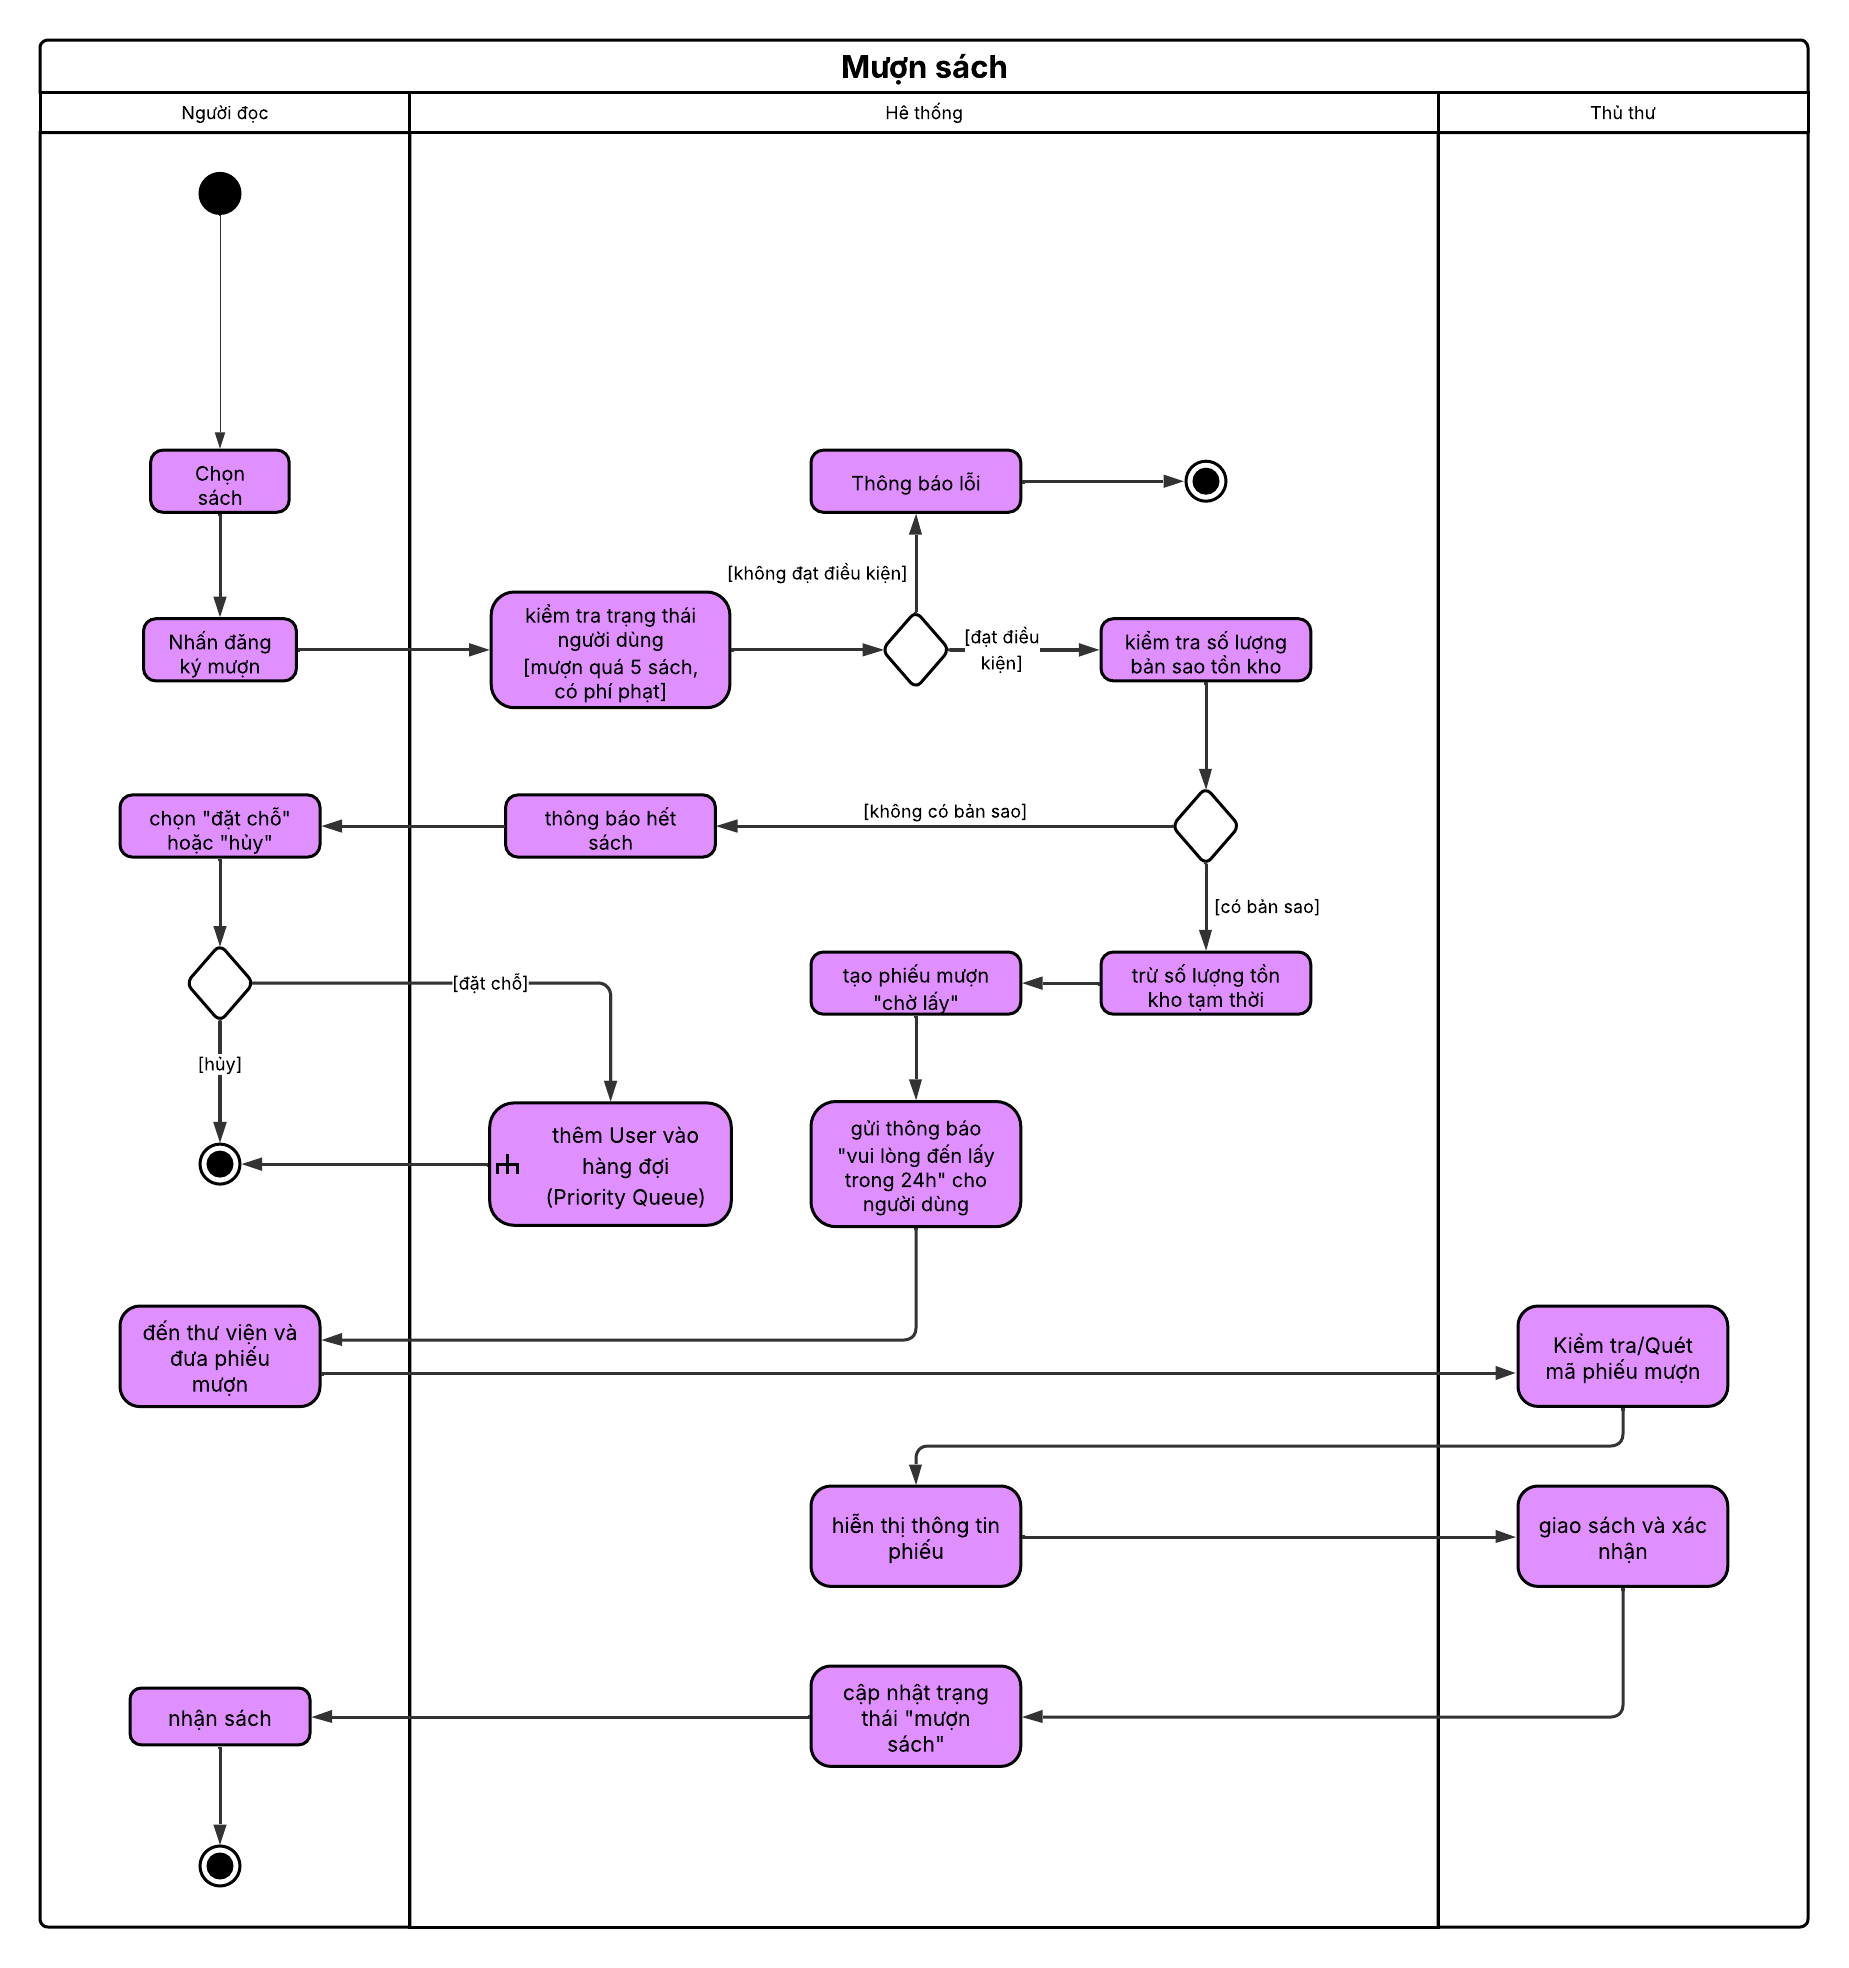
\includegraphics[width=\linewidth]{images/V.Analysis_and_Design/activity_diagram/borrow_book.png}
 \caption{Mượn sách — Activity Diagram}
 \label{fig:borrow_book}
\end{figure}

\begin{figure}[htbp]
 \centering
 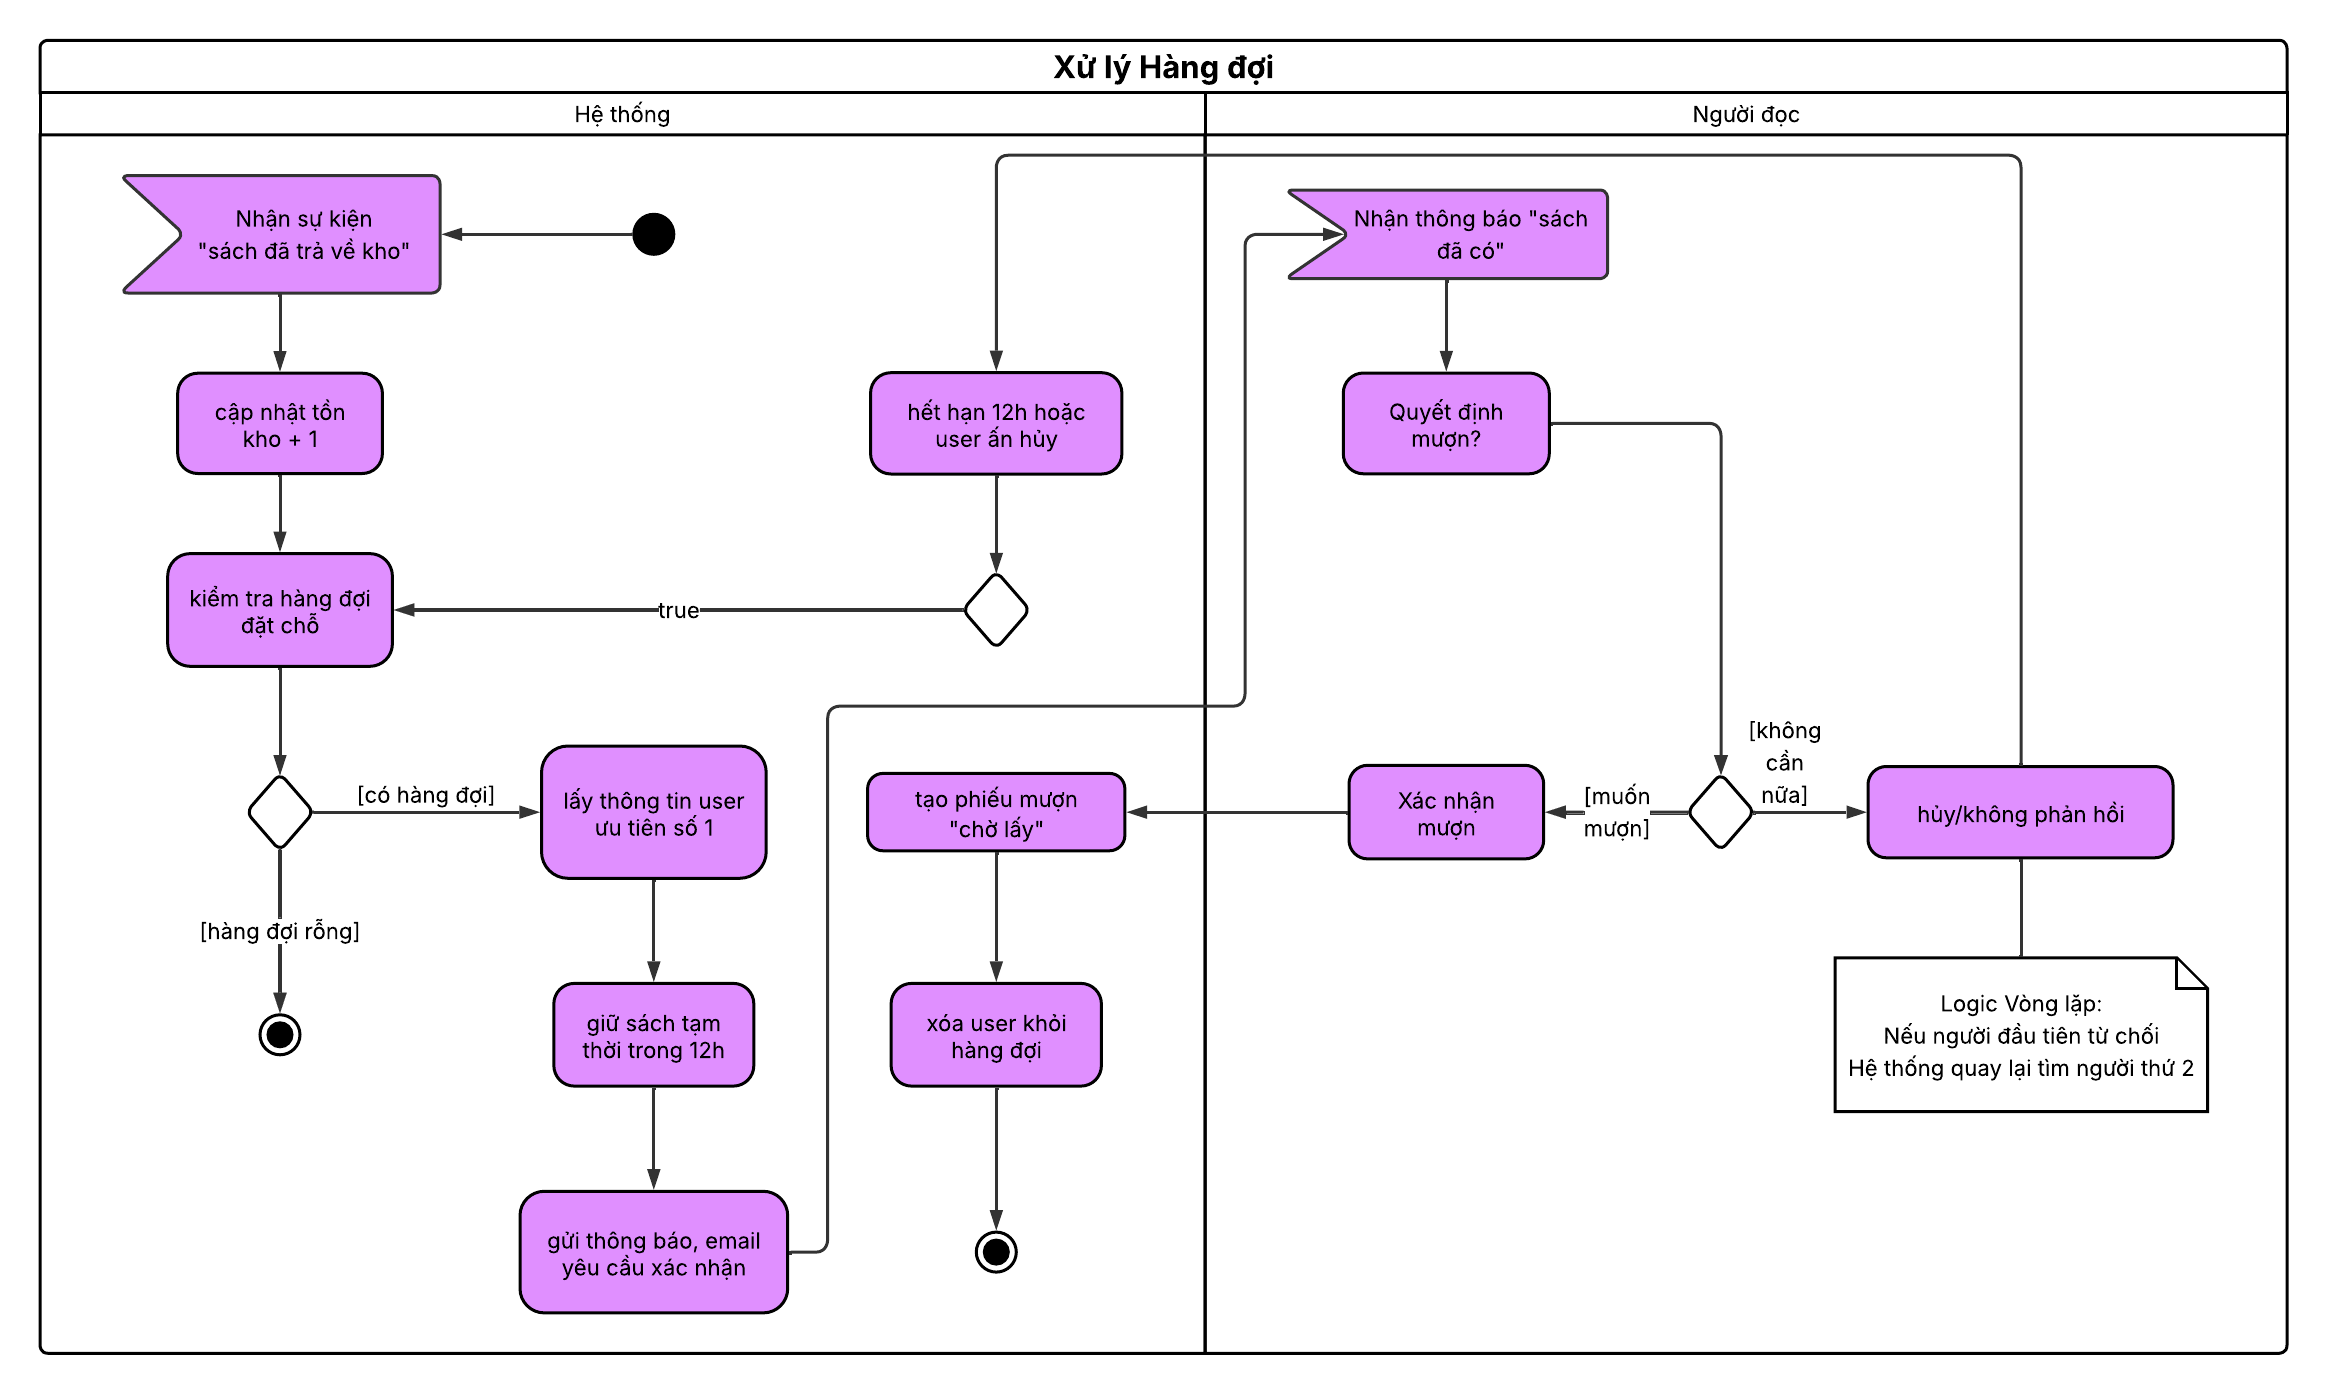
\includegraphics[width=\linewidth]{images/V.Analysis_and_Design/activity_diagram/process_queue.png}
 \caption{Xử lý hàng đợi — Activity Diagram}
 \label{fig:process_queue}
\end{figure}

\begin{figure}[htbp]
 \centering
 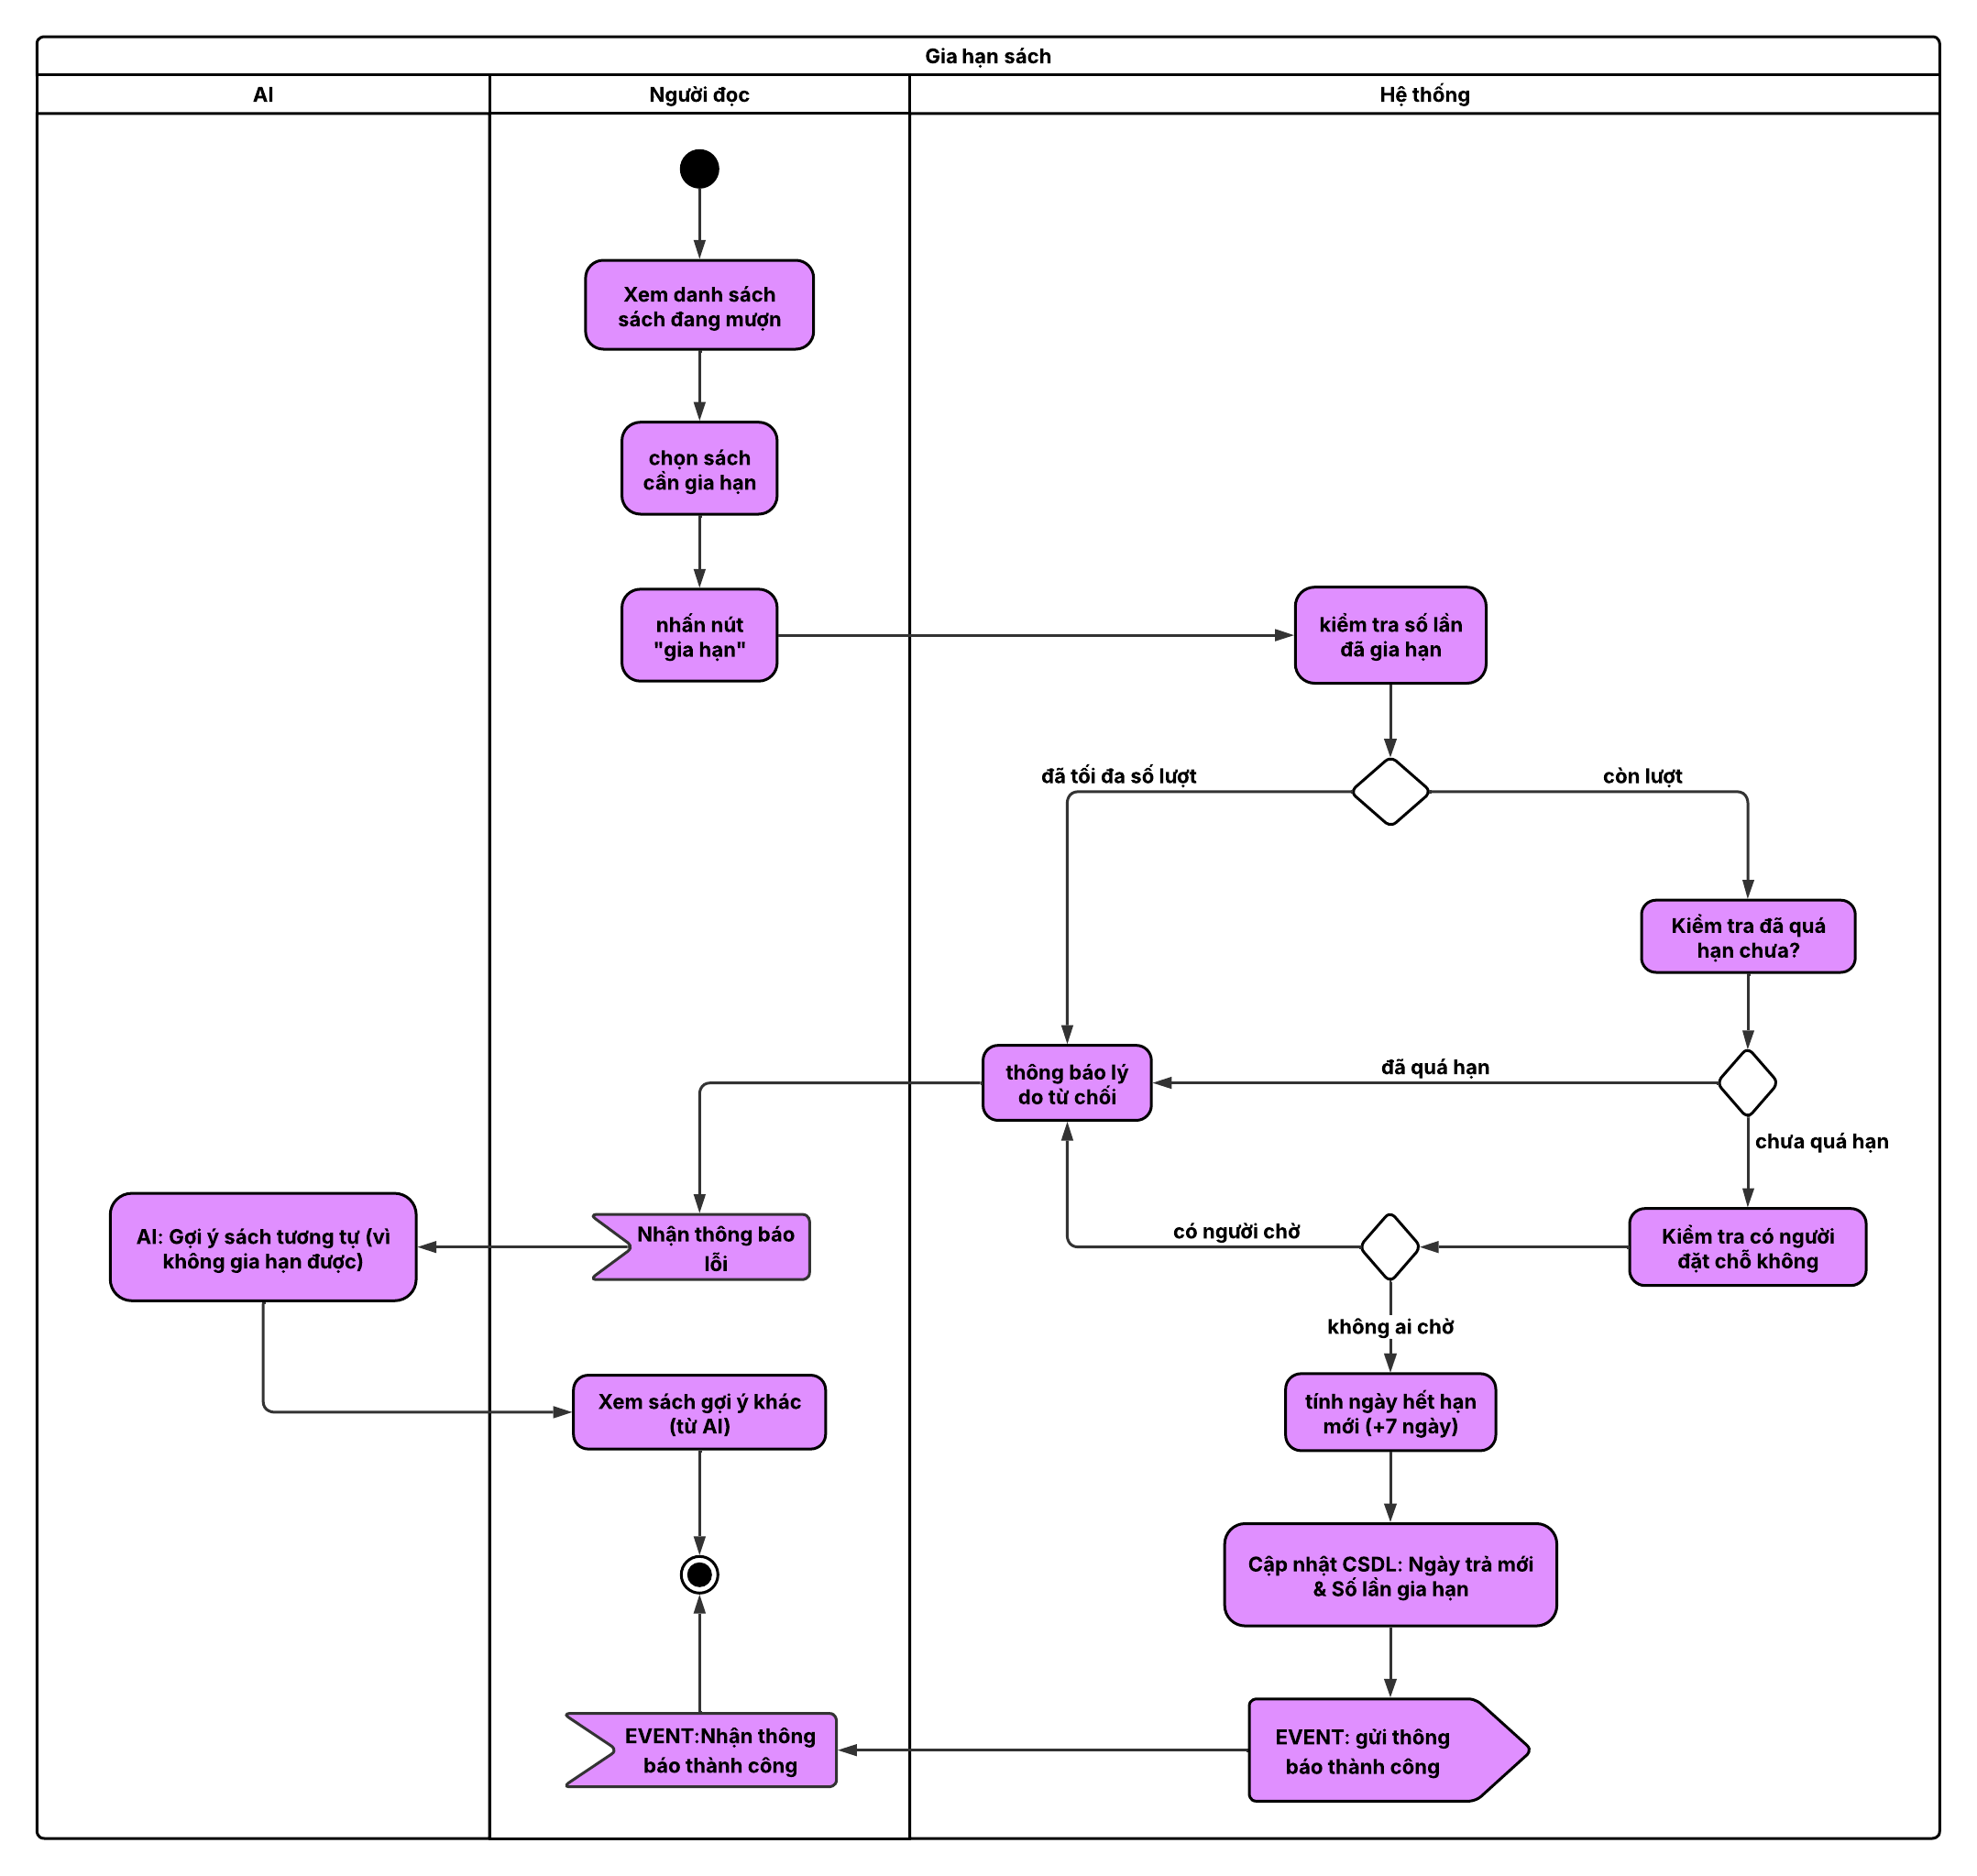
\includegraphics[width=\linewidth]{images/V.Analysis_and_Design/activity_diagram/gia_han_sach.png}
 \caption{Gia hạn sách — Activity Diagram}
 \label{fig:gia_han}
\end{figure}

\begin{figure}[htbp]
 \centering
 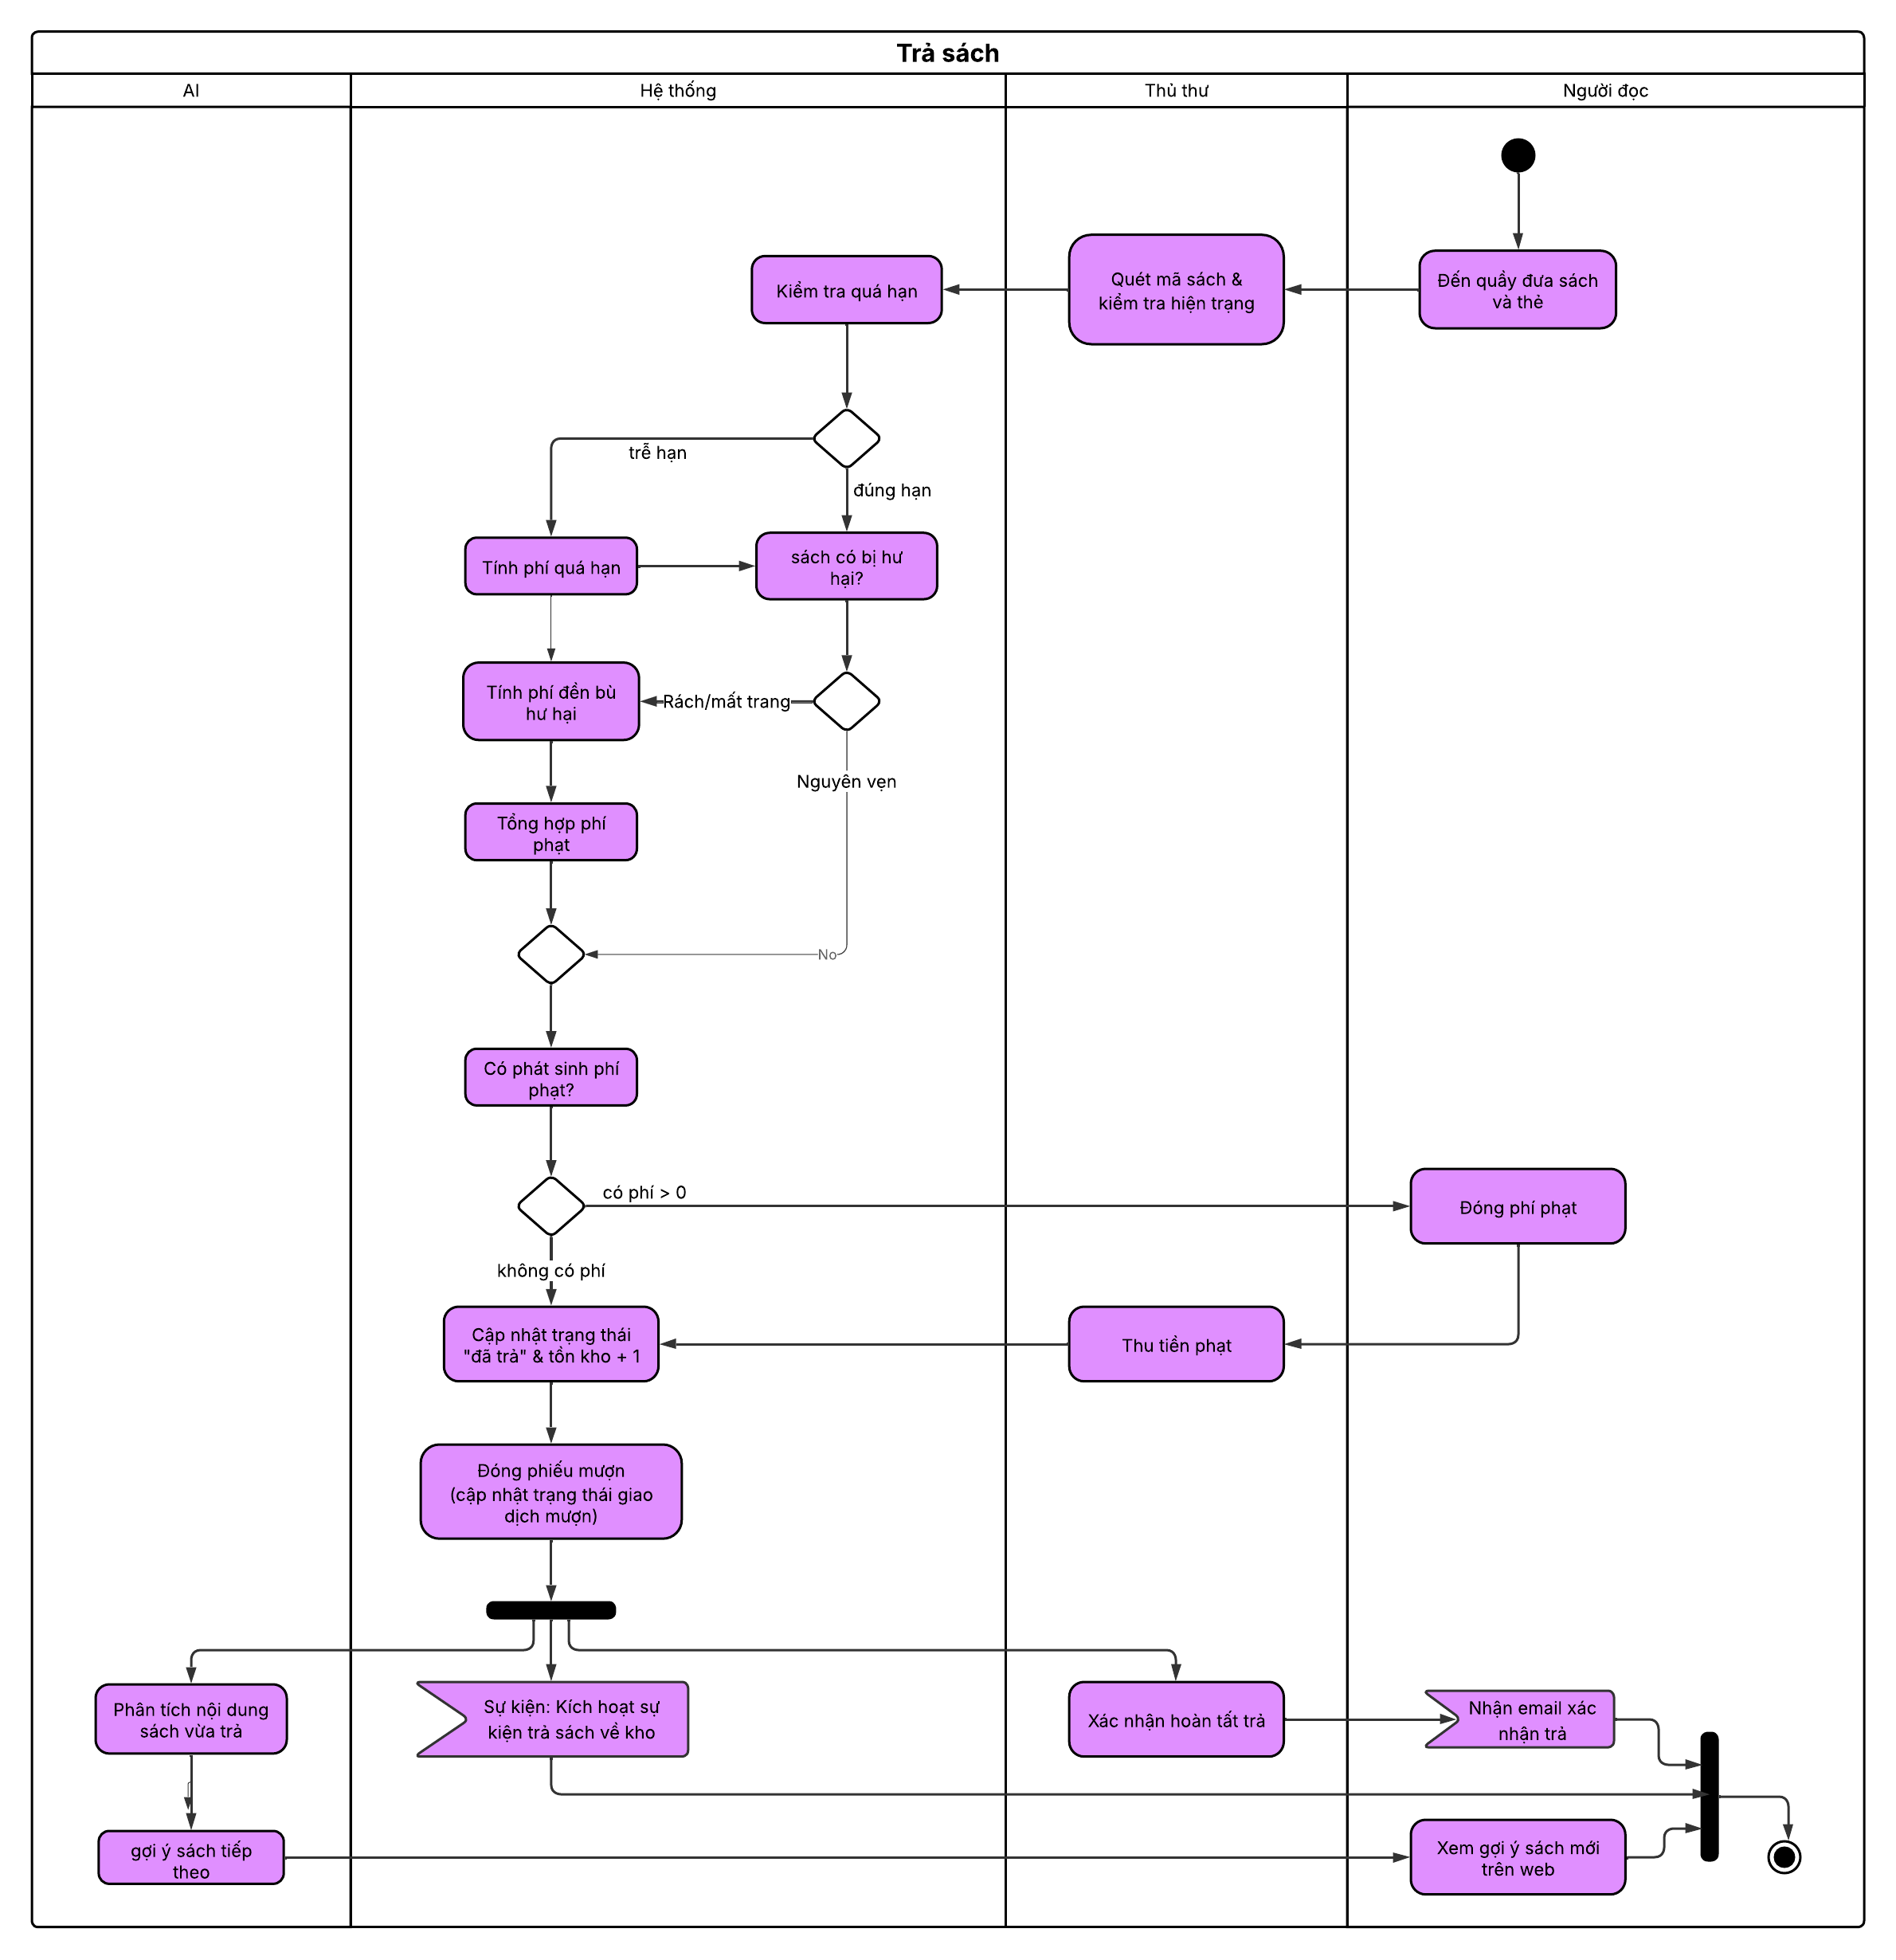
\includegraphics[width=\linewidth]{images/V.Analysis_and_Design/activity_diagram/return_book.png}
 \caption{Trả sách — Activity Diagram}
 \label{fig:return_book}
\end{figure}

\begin{figure}[htbp]
 \centering
 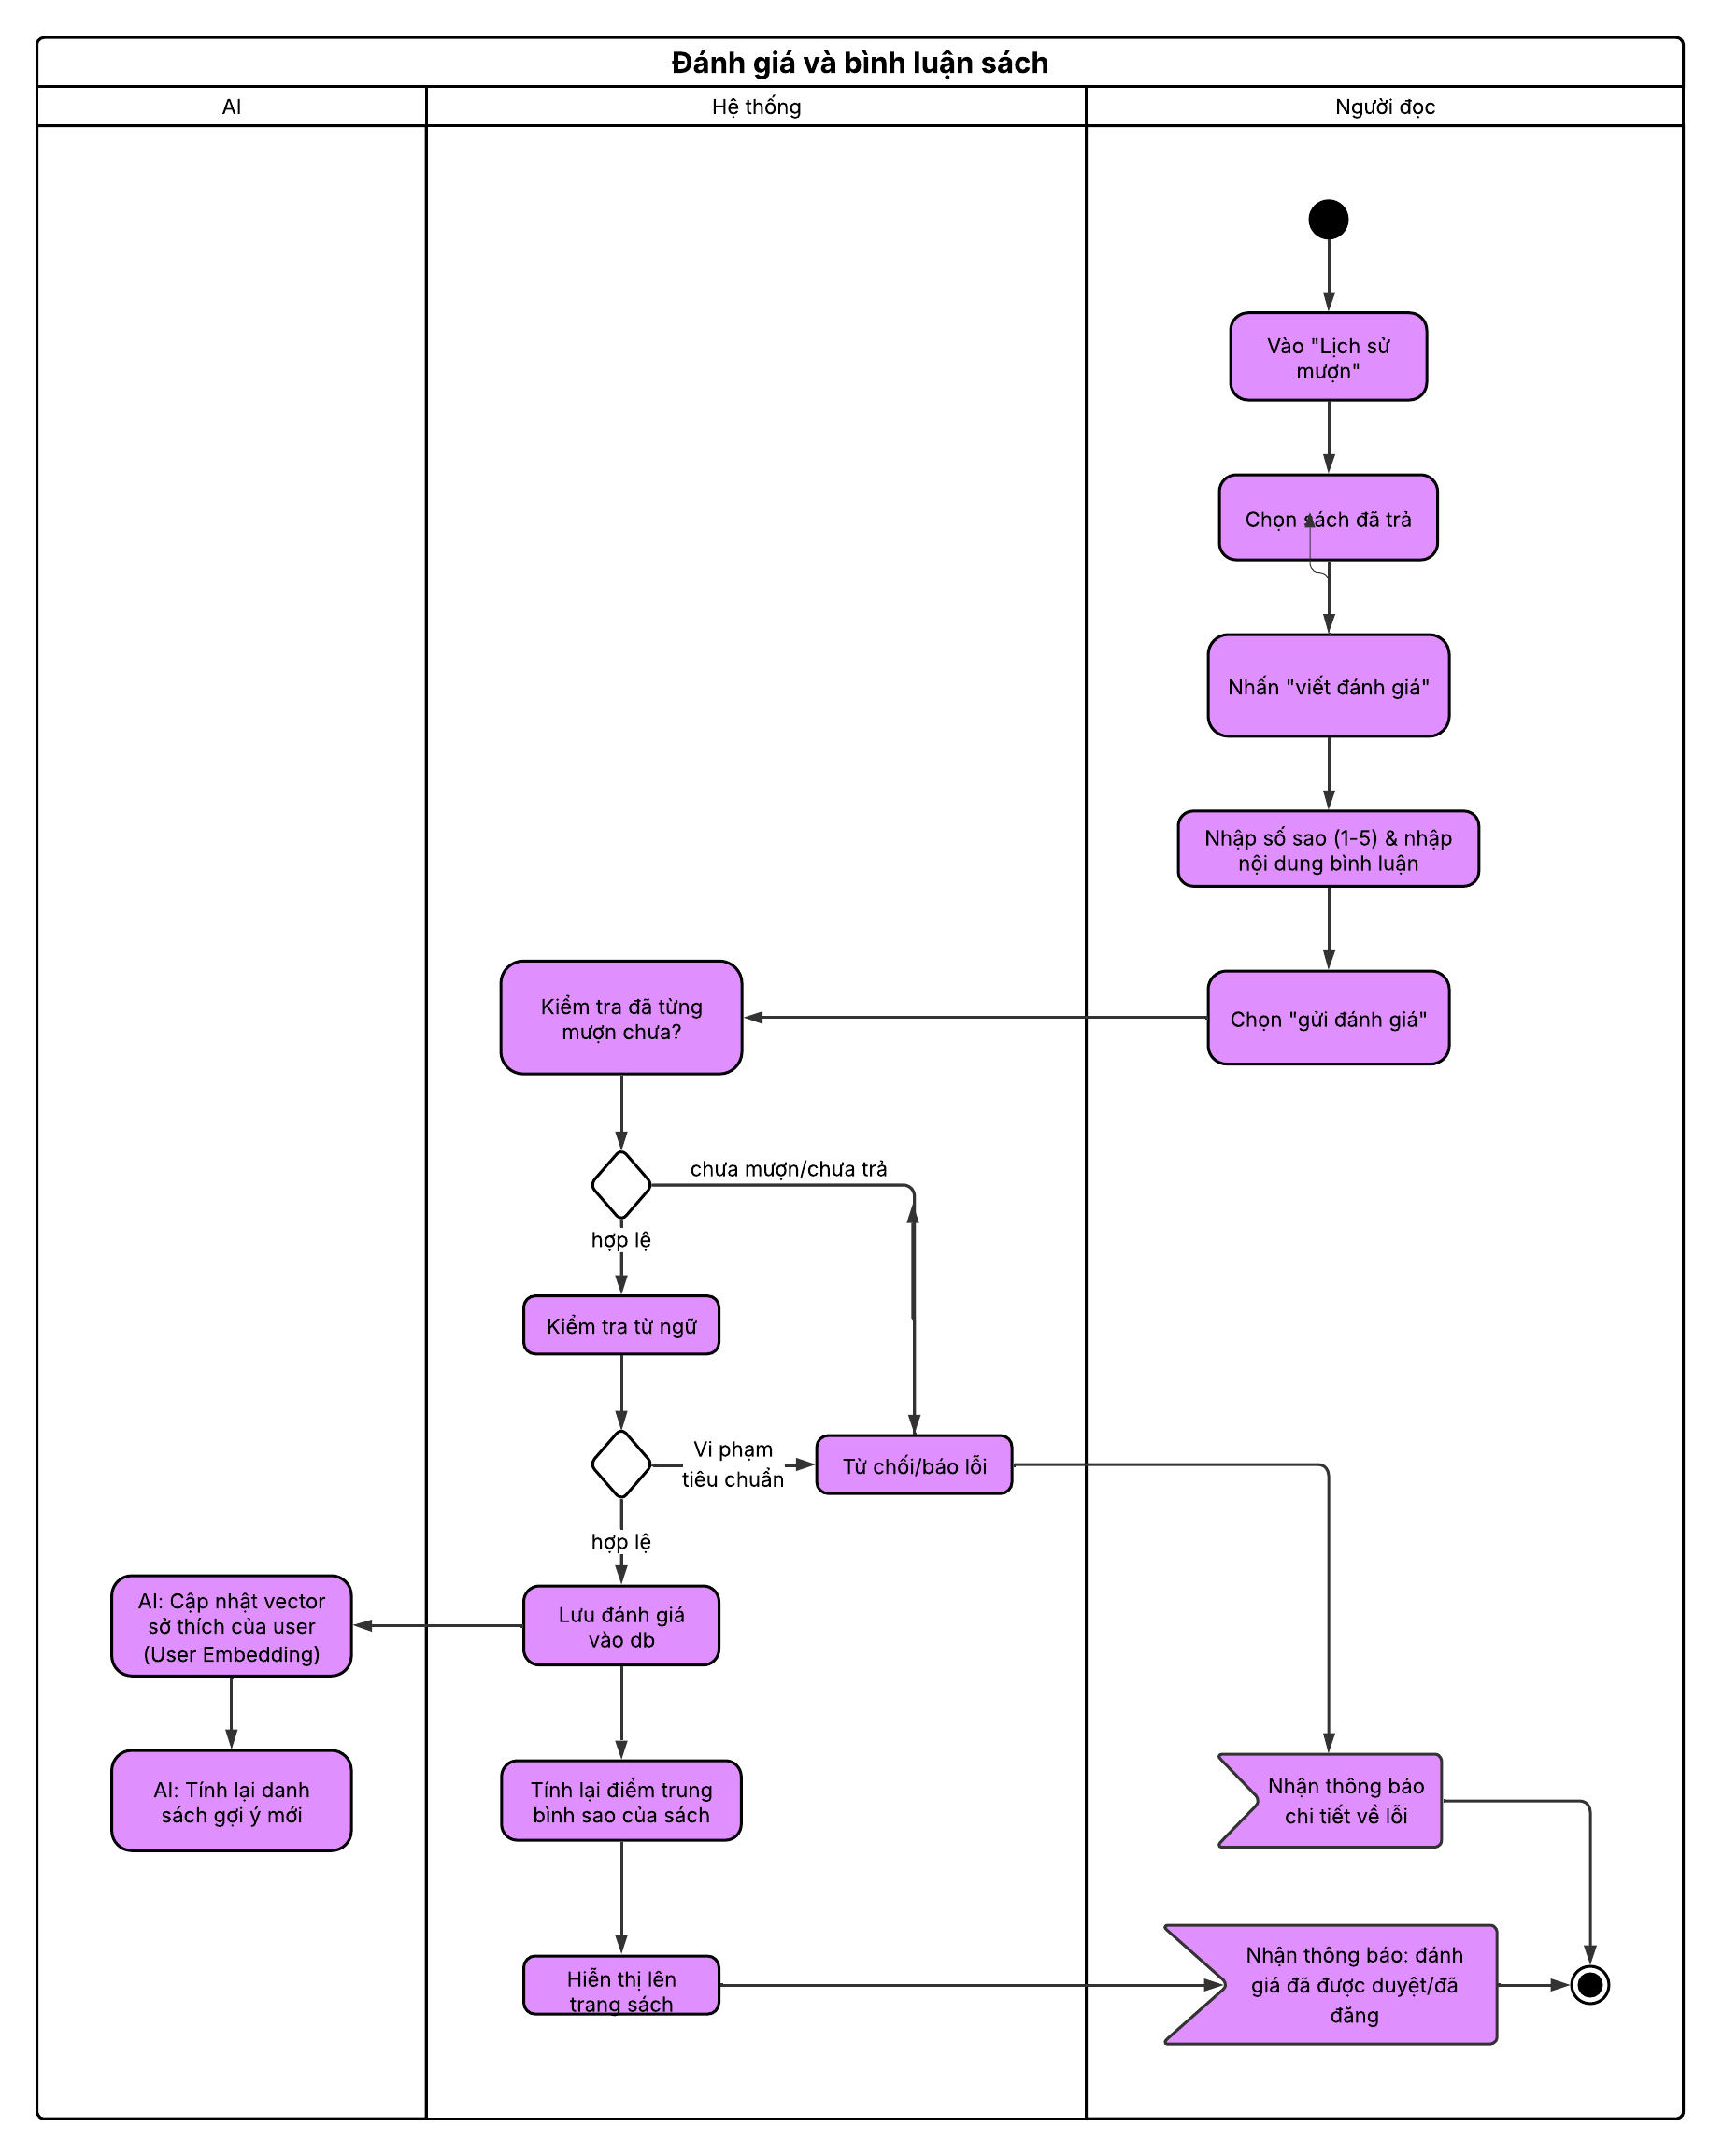
\includegraphics[width=\linewidth]{images/V.Analysis_and_Design/activity_diagram/review_and_comment.png}
 \caption{Đánh giá và bình luận sách — Activity Diagram}
 \label{fig:book_review_comment}
\end{figure}

\begin{figure}[htbp]
 \centering
 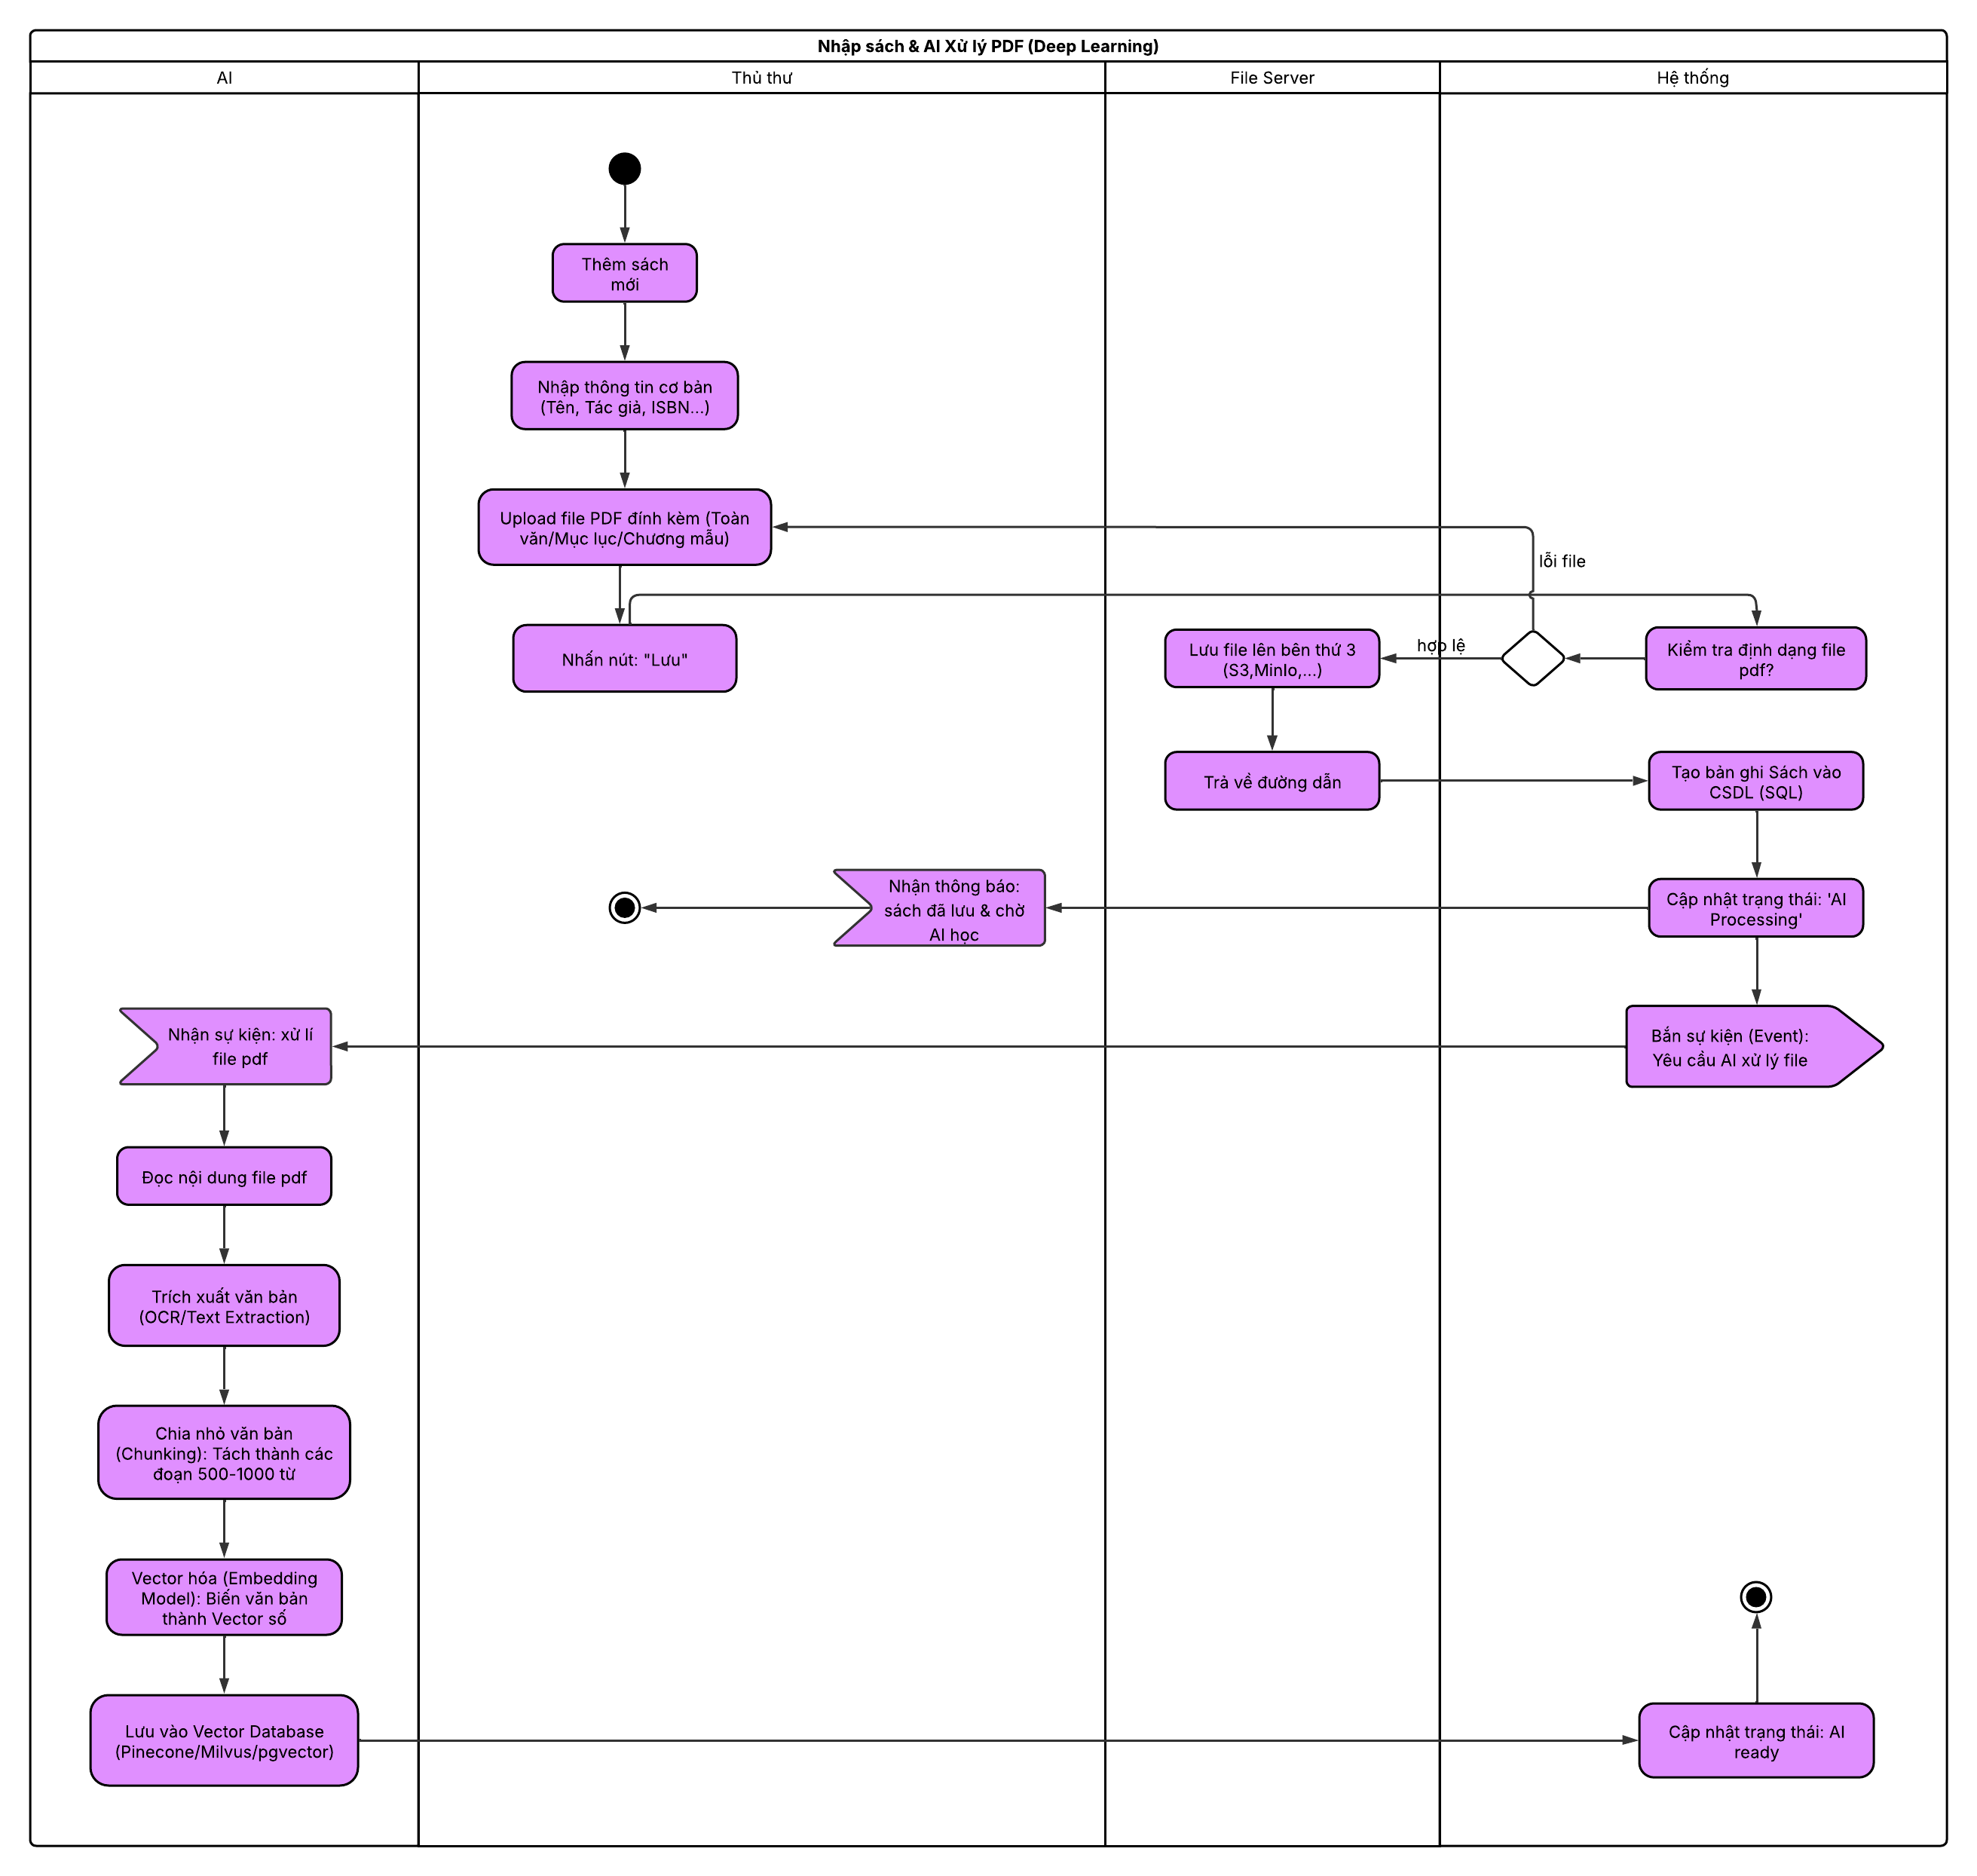
\includegraphics[width=\linewidth]{images/V.Analysis_and_Design/activity_diagram/add_book.png}
 \caption{Tạo sách với AI — Activity Diagram}
 \label{fig:create_book}
\end{figure}

\FloatBarrier

\section{Giải pháp công nghệ}
\label{sec:giai_phap_cong_nghe}

Mỗi lựa chọn công nghệ được đưa ra dựa trên bộ tiêu chí: (1) Hiệu năng \& độ trễ, (2) Khả năng mở rộng \& bảo trì, (3) Bảo mật \& phân quyền, (4) Trải nghiệm phát triển (DX) \& hệ sinh thái, (5) Chi phí \& mức độ phù hợp học thuật.

\subsection{Front-end}
\label{subsec:frontend_solution}

Kiến trúc Front-end được xây dựng dựa trên \textbf{React + Vite} — kết hợp giữa thư viện giao diện phổ biến nhất hiện nay (React) và công cụ build thế hệ mới với tốc độ cực nhanh (Vite). Sự lựa chọn này ưu tiên trải nghiệm phát triển (Developer Experience) vượt trội, tốc độ phản hồi tức thì trong quá trình lập trình, và khả năng triển khai đơn giản dưới dạng file tĩnh thông qua NGINX.

Để đưa ra quyết định công nghệ phù hợp nhất, nhóm đã tiến hành so sánh các nền tảng phổ biến dựa trên đặc thù của hệ thống. Dưới đây là bảng phân tích chi tiết.

\begin{table}[h!]
\centering
\setlength{\tabcolsep}{6pt}
\begin{tabularx}{\linewidth}{|>{\bfseries}l|>{\raggedright\arraybackslash}X|%
>{\raggedright\arraybackslash}X|%
>{\raggedright\arraybackslash}X|}
\hline
\textbf{Nền tảng} & \textbf{Ưu điểm} & \textbf{Nhược điểm} & \textbf{Lý do chọn/không chọn} \\
\hline
\textbf{React + Vite (Được chọn)} & Tốc độ HMR và build cực nhanh nhờ Vite (ESBuild), triển khai file tĩnh đơn giản qua NGINX, hệ sinh thái React phong phú, dễ tích hợp với mọi Backend API. & Client-side rendering thuần, SEO phụ thuộc vào cấu hình thêm, phải tự cấu hình Routing (React Router). & \textbf{Được chọn} vì hệ thống ưu tiên hiệu năng phát triển, triển khai nhẹ qua NGINX, và phần lớn giao diện là dashboard nội bộ không cần SEO. \\
\hline
Next.js & Hybrid Rendering (SSR/CSR/SSG), tối ưu SEO, hoạt động như BFF bảo mật. & Cần môi trường Node.js runtime để chạy, phức tạp hơn React thuần, tốn tài nguyên server hơn. & Không được chọn vì yêu cầu Node.js server riêng, phức tạp hóa việc triển khai khi hệ thống đã có Backend Spring Boot đảm nhận API. \\
\hline
Nuxt (Vue) & Mạnh mẽ tương đương Next.js trong hệ sinh thái Vue. & Cộng đồng doanh nghiệp nhỏ hơn React, ít thư viện UI hiện đại tương thích hơn. & Nhóm ưu tiên hệ sinh thái React do sự phổ biến và thư viện phong phú hơn. \\
\hline
Angular & Cấu trúc chặt chẽ, phù hợp Enterprise cực lớn. & \textbf{Độ phức tạp cao}, nhiều boilerplate, đường cong học tập dốc. & Quá cồng kềnh và cứng nhắc so với yêu cầu linh hoạt và phát triển nhanh của đồ án. \\
\hline
\end{tabularx}
\caption{Bảng so sánh các công nghệ Front-end}
\label{tab:frontend-compare}
\end{table}

\textbf{Lựa chọn:} \emph{React + Vite kết hợp với TypeScript, Tailwind CSS, Shadcn/ui, React Router và React Hook Form + Zod.}

\subsubsection*{Lý do chọn theo tiêu chí chuyên môn}

\begin{itemize}
    \item \textbf{Tốc độ phát triển vượt trội (Developer Experience):}
    Vite sử dụng ESBuild (viết bằng Go) để biên dịch, cho tốc độ khởi động server dev gần như tức thì và Hot Module Replacement (HMR) dưới 50ms bất kể kích thước dự án. So với Webpack truyền thống, thời gian build production giảm đáng kể, cho phép nhóm lập trình lặp nhanh hơn trong quá trình phát triển.

    \item \textbf{Triển khai đơn giản qua NGINX:}
    React + Vite tạo ra các file tĩnh (HTML/CSS/JS) sau khi build, có thể phục vụ trực tiếp bởi NGINX mà không cần Node.js server runtime. Điều này giúp giảm tài nguyên máy chủ, đơn giản hóa cấu hình Docker và tận dụng khả năng cache tĩnh của NGINX để tăng hiệu năng.

    \item \textbf{Phù hợp với đặc thù hệ thống:}
    Phần lớn giao diện của hệ thống là các trang Dashboard nội bộ (quản lý mượn/trả, quản lý độc giả, thống kê) dành cho người dùng đã đăng nhập — những trang này không cần SEO. Bảo mật API được đảm bảo ở phía Backend Spring Boot (JWT), nên không cần thêm một lớp Node.js BFF trung gian.

    \item \textbf{Hệ sinh thái React và tính an toàn dữ liệu:}
    Sự kết hợp giữa \textbf{TypeScript} (định kiểu tĩnh) và \textbf{Zod} (validation runtime) đảm bảo tính toàn vẹn dữ liệu khi giao tiếp với Backend API. Thư viện \textbf{Shadcn/ui} (dựa trên Radix UI) và \textbf{Tailwind CSS} giúp xây dựng giao diện đẹp, nhất quán và dễ tiếp cận (Accessible) với lượng code tối thiểu.

    \item \textbf{Quản lý trạng thái và Routing:}
    \textbf{React Router v6} cung cấp hệ thống routing linh hoạt với Data Loaders và Error Boundaries tích hợp. Kết hợp với \textbf{TanStack Query} để quản lý server state và cache dữ liệu từ API, giúp giảm số lần gọi API trùng lặp và đồng bộ trạng thái giao diện tự động.
\end{itemize}


\subsection{Back-end}
\label{subsec:backend_solution}

Kiến trúc Back-end được xây dựng tập trung vào sự ổn định, an toàn và khả năng xử lý các nghiệp vụ phức tạp của thư viện.

\begin{table}[h!]
\centering
\setlength{\tabcolsep}{6pt}
\begin{tabularx}{\linewidth}{|>{\bfseries}l|>{\raggedright\arraybackslash}X|%
>{\raggedright\arraybackslash}X|%
>{\raggedright\arraybackslash}X|}
 \hline
 \textbf{Nền tảng}
& \textbf{Ưu điểm}
& \textbf{Nhược điểm}
& \textbf{Lý do không được chọn} \\
 \hline
 \textbf{Spring Boot (Được chọn)}
& \textbf{Ổn định, bảo mật cao}, hệ sinh thái Java mạnh mẽ, \textbf{quản lý giao dịch} và dữ liệu quan hệ (JPA) rất tốt.
& Có thể hơi “dài dòng” hơn so với các framework khác.
& N/A \\
 \hline
 NestJS / Express
& Linh hoạt, hiệu năng tốt, sử dụng chung ngôn ngữ JavaScript/TypeScript với front-end.
& Việc xử lý các nghiệp vụ quan hệ phức tạp và giao dịch không mạnh mẽ bằng Spring Boot.
& Spring Boot phù hợp hơn với bản chất dữ liệu quan hệ và giao dịch chặt chẽ của nghiệp vụ thư viện. \\
 \hline
 Django / DRF
& Phát triển CRUD cực nhanh, hệ sinh thái Python mạnh.
& Nhóm phát triển quen thuộc với hệ sinh thái Java hơn.
& Stack công nghệ Java đã quen thuộc và đồng bộ hơn với kinh nghiệm của nhóm. \\
 \hline
 MongoDB (NoSQL)
& Schema linh hoạt, dễ dàng mở rộng theo chiều ngang.
& \textbf{Không phù hợp} với các mối quan hệ dữ liệu chặt chẽ và yêu cầu giao dịch cao của hệ thống thư viện.
& Bản chất nghiệp vụ của dự án phù hợp hơn với cơ sở dữ liệu quan hệ (RDBMS). \\
 \hline
\end{tabularx}
\caption{Bảng so sánh các công nghệ Back-end}
\label{tab:backend-compare}
\end{table}

\textbf{Lựa chọn:} \emph{Spring Boot 3 (Java 21), Spring Security (JWT), Spring Data JPA, PostgreSQL, Redis, và OpenAPI/Swagger. Mô-đun AI/NLP được tách thành một service riêng sử dụng Python (FastAPI).}

\subsubsection*{Lý do chọn theo tiêu chí chuyên môn}
\begin{itemize}
 \item \textbf{Độ tin cậy và Hiệu năng:} Spring Boot là một framework đã được kiểm chứng về độ ổn định và hiệu năng trong các hệ thống enterprise. Kết hợp với \textbf{Java Virtual Machine (JVM)}, nó cung cấp khả năng xử lý đồng thời (concurrency) mạnh mẽ, phù hợp với các tác vụ CRUD và giao dịch (transactions) phức tạp. Việc sử dụng \textbf{Redis} làm lớp cache giúp giảm tải cho cơ sở dữ liệu đối với các truy vấn tốn kém hoặc thường xuyên (ví dụ: gợi ý, top sách).

 \item \textbf{Mô hình Dữ liệu và Khả năng mở rộng:} Nghiệp vụ thư viện có bản chất là quan hệ chặt chẽ. \textbf{Spring Data JPA} và \textbf{Hibernate} cung cấp một tầng ORM (Object-Relational Mapping) mạnh mẽ, cho phép mô hình hóa các thực thể và mối quan hệ phức tạp một cách tự nhiên. Việc sử dụng \textbf{Specification Pattern} giúp xây dựng các truy vấn động một cách an toàn và dễ bảo trì, phục vụ cho các yêu cầu lọc và tìm kiếm phức tạp.

 \item \textbf{Bảo mật Toàn diện:} \textbf{Spring Security} là một framework bảo mật hàng đầu, cho phép triển khai cơ chế xác thực và phân quyền một cách linh hoạt. Việc sử dụng \textbf{JWT (JSON Web Tokens)} với cặp \textbf{Access/Refresh Token} đảm bảo một cơ chế xác thực stateless, phù hợp với kiến trúc API hiện đại. Luồng bảo mật được thiết kế để token không bao giờ được lưu trữ ở client-side storage, thay vào đó là sử dụng \textbf{HttpOnly cookies} để giảm thiểu rủi ro từ các cuộc tấn công \textbf{Cross-Site Scripting (XSS)}.

 \item \textbf{Kiến trúc Microservice cho AI:} Việc tách mô-đun AI/NLP (tìm kiếm ngữ nghĩa, gợi ý) thành một service riêng (Python/FastAPI) là một quyết định kiến trúc chiến lược. Nó cho phép hai hệ thống có thể được phát triển, triển khai và mở rộng quy mô một cách độc lập. Python và hệ sinh thái của nó là lựa chọn tối ưu cho các tác vụ Machine Learning, trong khi Java/Spring Boot mạnh hơn về xử lý nghiệp vụ.
\end{itemize}

\subsection*{Kết luận về Sự phối hợp giữa hai nền tảng}
Kiến trúc tổng thể được thiết kế theo mô hình \textbf{đầu-cuối (end-to-end) an toàn và hiệu quả}. \textbf{Next.js} hoạt động như một lớp BFF, chịu trách nhiệm render giao diện và giao tiếp an toàn với \textbf{Spring Boot API}. Luồng xác thực sử dụng \textbf{HttpOnly cookies} để vận chuyển JWT, đảm bảo token không thể bị truy cập bởi mã JavaScript độc hại trên trình duyệt. Sự phân tách rõ ràng giữa các thành phần không chỉ giúp tối ưu hiệu năng mà còn tạo ra một hệ thống linh hoạt, dễ bảo trì và sẵn sàng cho việc mở rộng trong tương lai.



%--- ỨNG DỤNG AI VÀO PROJECT ---%


\section{Ứng dụng AI vào hệ thống}
% =========================================================================================
\textbf{Bối cảnh và Mục tiêu} \\ 
Mục tiêu cốt lõi là chuyển đổi trải nghiệm từ \textbf{"Tìm kiếm" (Searching)} sang \textbf{"Khám phá" (Discovering)}. Hệ thống sử dụng AI để thấu hiểu hành vi người dùng và nội dung sách, từ đó đưa ra các gợi ý phù hợp ngay cả khi người dùng chưa xác định rõ nhu cầu. \\ 
Để giải quyết bài toán gợi ý và tìm kiếm ngữ nghĩa trong thời gian thực, hệ thống được thiết kế theo kiến trúc Microservices lai. Logic AI được tách biệt hoàn toàn khỏi Core Backend để đảm bảo hiệu năng và khả năng mở rộng.

\begin{figure}[htbp]
\centering
\begin{tikzpicture}[
    node distance=1.5cm,
    every node/.style={font=\small},
    % Styles
    client/.style={rectangle, draw=blue!60, fill=blue!5, very thick, minimum size=1cm, rounded corners, align=center},
    backend/.style={rectangle, draw=green!60!black, fill=green!5, very thick, minimum width=3.5cm, minimum height=1.5cm, rounded corners, align=center},
    aiservice/.style={rectangle, draw=red!60, fill=red!5, very thick, minimum width=3.5cm, minimum height=1.5cm, rounded corners, align=center},
    database/.style={cylinder, draw=orange!60, fill=orange!5, shape border rotate=90, aspect=0.25, minimum height=2cm, minimum width=2cm, very thick, align=center},
    arrow/.style={thick, ->, >=stealth}
]

    % Nodes
    \node[client] (user) {Client App\\(Next.js)};
    \node[backend, right=2cm of user] (springboot) {\textbf{Core Backend}\\(Spring Boot)\\Quản lý nghiệp vụ};
    \node[aiservice, right=2cm of springboot] (fastapi) {\textbf{AI Service}\\(Python/FastAPI)\\Xử lý tính toán};
    \node[database, below=1.5cm of springboot] (postgres) {\textbf{PostgreSQL}\\+ pgvector\\(Lưu trữ tập trung)};
    
    % Edges
    \draw[arrow] (user) -- node[above] {REST API} (springboot);
    \draw[arrow] (springboot) -- node[above] {Internal API} (fastapi);
    \draw[arrow] (springboot) -- node[left] {CRUD} (postgres);
    \draw[arrow] (fastapi) |- node[right, near start] {Vector Query} (postgres);

    % Labels
    \node[below=0.2cm of user] {\textit{User Interaction}};

\end{tikzpicture}
\caption{Kiến trúc tích hợp hệ thống}
\label{fig:architecture}
\end{figure}

\textbf{Đặc tả luồng dữ liệu:}
\begin{itemize}
    \item \textbf{Spring Boot (Business Layer):} Chịu trách nhiệm ghi nhận tương tác người dùng (User Interaction) và gửi yêu cầu phân tích sang AI Service. Việc tách biệt này giúp hệ thống nghiệp vụ vẫn hoạt động ổn định ngay cả khi AI Service đang quá tải \cite{nhatthanh2025cleanblog}.
    \item \textbf{AI Service (Intelligence Layer):} Được xây dựng bằng Python/FastAPI để tận dụng hệ sinh thái thư viện AI mạnh mẽ (PyTorch, Scikit-learn). Service này chạy các Batch Job định kỳ để huấn luyện mô hình và cung cấp API thời gian thực cho tính toán gợi ý.
    \item \textbf{PostgreSQL + pgvector (Data Layer):} Nhóm lựa chọn giải pháp lưu trữ "All-in-one" thay vì sử dụng Vector Database chuyên biệt (như Pinecone hay Milvus). Lý do là để đơn giản hóa kiến trúc và tận dụng khả năng truy vấn hỗn hợp (Hybrid Search) - kết hợp giữa lọc theo siêu dữ liệu (metadata filtering) và tìm kiếm vector trong cùng một câu lệnh SQL \cite{pgvector_docs}.
\end{itemize}

% =========================================================================================
\subsection{Module 1: Tìm kiếm ngữ nghĩa (Semantic Search)} 
\subsubsection{Cơ sở Lý thuyết: Text Embedding}
Hệ thống sử dụng kỹ thuật \textbf{Dense Retrieval} thay vì Keyword Matching truyền thống (như SQL \texttt{LIKE} hay BM25). Các phương pháp cũ như TF-IDF hay GloVe \cite{Pennington2014GloVe} gặp hạn chế lớn trong việc hiểu ngữ cảnh của câu (context-aware), vì chúng chỉ biểu diễn từ đơn lẻ hoặc không thay đổi theo ngữ cảnh (static embeddings) \cite{Mikolov2013Efficient}.

Công nghệ lõi nhóm lựa chọn là \textbf{Sentence-BERT (SBERT)} \cite{Reimers2019SentenceBERT}, một biến thể của BERT \cite{Devlin2019BERT} sử dụng kiến trúc mạng Siamese (Siamese Networks) để tinh chỉnh (fine-tune) việc tạo ra các sentence embedding.
\textbf{Lý giải lựa chọn SBERT (Sentence-BERT):}  \\
\begin{itemize}
\item Mặc dù BERT \cite{Devlin2019BERT} đạt hiệu quả cao trong các tác vụ NLP, nhưng nó sử dụng kiến trúc Cross-Encoder, yêu cầu đưa cả hai câu vào mạng cùng lúc để so sánh. Điều này dẫn đến độ phức tạp tính toán khổng lồ khi tìm kiếm trong cơ sở dữ liệu lớn.  
\item Theo Reimers và Gurevych \cite{Reimers2019SentenceBERT}, nhóm sử dụng kiến trúc \textbf{Bi-Encoder} của SBERT để tính toán vector độc lập cho từng văn bản. Điều này cho phép tính toán trước (Pre-compute) vector cho toàn bộ kho sách, chuyển bài toán tìm kiếm về bài toán tìm láng giềng gần nhất (ANN), đảm bảo thời gian phản hồi thời gian thực. 

\end{itemize}
% -----------------------------------------

\textbf{Mô hình toán học:}
Mô hình biến đổi một đoạn văn bản $T$ (Text) thành một vector số học cố định $v \in \mathbb{R}^{768}$:
\begin{equation}
    f_{\text{SBERT}}(T) \rightarrow v = [x_1, x_2, \dots, x_{768}]
\end{equation}
Trong đó, độ tương đồng giữa câu truy vấn $q$ và tài liệu $d$ được tính bằng \textbf{Cosine Similarity}:
\begin{equation}
    \text{sim}(q, d) = \frac{v_q \cdot v_d}{\|v_q\| \|v_d\|} = \frac{\sum_{i=1}^{n} q_i d_i}{\sqrt{\sum_{i=1}^{n} q_i^2} \sqrt{\sum_{i=1}^{n} d_i^2}}
\end{equation}


\textbf{Ví dụ:} Mô hình biến đổi một đoạn văn bản (Text) thành một vector số học cố định (Vector) trong không gian nhiều chiều (768 chiều).
\begin{equation}
    f(\text{"Lập trình C++"}) \rightarrow [0.12, -0.59, 0.21, ..., 0.05]
\end{equation}
Các văn bản có ngữ nghĩa gần nhau sẽ có vector nằm gần nhau trong không gian này.
\subsubsection{Quy trình Xử lý Dữ liệu Sách (ETL Pipeline)}
Để chuyển đổi một file PDF "vô tri" thành các thực thể có ý nghĩa trong cơ sở dữ liệu, nhóm thiết kế một quy trình ETL gồm 4 giai đoạn: \textbf{Ingestion} (Thu thập) $\rightarrow$ \textbf{Processing} (Xử lý) $\rightarrow$ \textbf{Enrichment} (Làm giàu) $\rightarrow$ \textbf{Embedding} (Vector hóa).

\begin{figure}[htbp]
\centering
\begin{tikzpicture}[
    node distance=1.5cm,
    auto,
    % Styles
    % Styles
    stage/.style={rectangle, draw=blue!80, fill=blue!5, very thick, minimum width=3.5cm, minimum height=1.5cm, align=center, rounded corners, font=\small\bfseries},
    action/.style={rectangle, draw=black!60, fill=white, dashed, minimum width=3cm, align=center, font=\footnotesize, minimum height=2cm},
    arrow/.style={thick, ->, >=stealth}
]
    \node[stage] (s1) {Giai đoạn 1\\Ingestion\\(Đầu vào)};
    \node[stage, right=1.5cm of s1] (s2) {Giai đoạn 2\\Processing\\(Tiền xử lý)};
    \node[stage, below=3.5cm of s2] (s3) {Giai đoạn 3\\Enrichment\\(AI Phân tích)};
    \node[stage, left=1.5cm of s3] (s4) {Giai đoạn 4\\Embedding\\(Vector hóa)};

    \node[action, below=0.2cm of s1] (a1) {Input: File PDF\\Công cụ: PyMuPDF\\Output: Raw Text};
    \node[action, below=0.2cm of s2] (a2) {Kỹ thuật: Sliding Window\\Size: 1000 tokens\\Overlap: 200 tokens};
    \node[action, below=0.2cm of s3] (a3) {Công cụ: LLM (Gemini)\\Tác vụ: Tóm tắt, Tagging,\\Target Audience};
    \node[action, below=0.2cm of s4] (a4) {Model: SBERT\\(vietnamese-bi-encoder)\\Output: Vector [768]};
    
    \draw[arrow] (s1) -- (s2);
    \draw[arrow] (s2.east) -| ++(1.5,0) |- (s3.north);
    \draw[arrow] (s3) -- (s4);
    
\end{tikzpicture}
\caption{Quy trình Vector hóa nội dung sách}
\end{figure}

\textbf{Giai đoạn 1: Ingestion (Trích xuất)}
Sử dụng thư viện \texttt{PyMuPDF} để đọc nội dung file PDF. Hệ thống áp dụng Regular Expression (Regex) để loại bỏ nhiễu (header, footer, số trang) nhằm đảm bảo văn bản sạch trước khi đưa vào xử lý.

\textbf{Giai đoạn 2: Processing (Cắt đoạn)}
Vì giới hạn đầu vào của các mô hình ngôn ngữ (Context Window), chúng ta không thể đưa cả cuốn sách vào một lần.
\begin{itemize}
    \item \textbf{Kỹ thuật:} \textit{Sliding Window} (Cửa sổ trượt).
    \item \textbf{Thông số:} Kích thước đoạn (Chunk size) là 1000 tokens, với độ chồng lấn (Overlap) là 200 tokens.
    \item \textbf{Mục đích:} Đảm bảo không làm đứt gãy mạch văn hoặc mất ngữ cảnh quan trọng tại các điểm cắt.
\end{itemize}

\textbf{Giai đoạn 3: Enrichment (Làm giàu dữ liệu)}
Nhóm sử dụng \textbf{Large Language Model (LLM)} để trích xuất thông tin ẩn mà các phương pháp NLP truyền thống khó làm được. Prompt Engineering được thiết kế để trả về cấu trúc JSON nghiêm ngặt, giúp dễ dàng tích hợp vào Database.

\textbf{Mẫu Prompt gửi cho LLM:}
\begin{verbatim}
PROMPT = """
Đọc nội dung sau từ cuốn sách và thực hiện các tác vụ:
1. Tóm tắt nội dung chính (Summary) trong khoảng 150 từ.
2. Xác định 5 Tags (Thẻ) quan trọng nhất mô tả chủ đề.
3. Xác định Đối tượng độc giả phù hợp (Target Audience).
4. Trả về định dạng JSON (không kèm markdown):
{
    "summary": "...",
    "tags": ["...", "..."],
    "target_audience": ["...", "..."]
}
"""
\end{verbatim}

\textbf{Ví dụ kết quả thực tế (Sách "Clean Code"):}
\begin{itemize}
    \item \textbf{Summary:} "Cuốn sách hướng dẫn các nguyên tắc và thực hành để viết mã sạch, dễ bảo trì và mở rộng. Tác giả nhấn mạnh vào việc đặt tên biến, refactoring và kiểm thử đơn vị."
    \item \textbf{Tags:} \texttt{["Software Engineering", "Refactoring", "Java", "Best Practices", "Agile"]}
    \item \textbf{Target Audience:} \texttt{["Lập trình viên", "Kỹ sư phần mềm", "Sinh viên CNTT năm cuối"]}
\end{itemize}

\textbf{Giai đoạn 4: Embedding và Lưu trữ}
Cuối cùng, phần \texttt{summary} (đã được cô đọng) sẽ được vector hóa.
\begin{itemize}
    \item \textbf{Model:} Sử dụng \texttt{bkai-foundation-models/vietnamese-bi-encoder} (hoặc mô hình tương đương hỗ trợ tiếng Việt tốt).
    \item \textbf{Output:} Vector $v \in \mathbb{R}^{768}$.
    \item \textbf{Lưu trữ:} Vector này được lưu vào cột \texttt{embedding} kiểu \texttt{vector(768)} trong PostgreSQL.
    \item \textbf{Tối ưu:} Sử dụng chỉ mục \textbf{HNSW} (Hierarchical Navigable Small World) để tăng tốc độ truy vấn vector thay vì quét toàn bộ bảng.
\end{itemize}


\subsubsection{Thuật toán Tìm kiếm}
Khi người dùng nhập câu truy vấn $q$:
\begin{enumerate}
    \item AI Service chuyển $q$ thành vector $v_q$.
    \item Tính độ tương đồng Cosine giữa $v_q$ và tất cả vector sách $v_d$ trong Database.
    \begin{equation}
        \text{Similarity}(v_q, v_d) = \frac{v_q \cdot v_d}{\|v_q\| \|v_d\|}
    \end{equation}
    \item Trả về danh sách sách có độ tương đồng cao nhất.
\end{enumerate}
Khi người dùng thực hiện tìm kiếm, hệ thống không so khớp từ khóa đơn thuần mà so khớp ý định (Semantic Match).

\begin{figure}[htbp]
\centering
\begin{tikzpicture}[
    node distance=2.5cm,
    auto,
    % Styles - Added align=center to fix LR mode error
    user/.style={circle, draw=black, fill=yellow!20, thick, minimum size=1.2cm, align=center},
    system/.style={rectangle, draw=black, fill=blue!10, thick, minimum width=3.5cm, minimum height=1.5cm, rounded corners, align=center},
    db/.style={cylinder, draw=black, fill=orange!10, shape border rotate=90, aspect=0.25, minimum height=2cm, minimum width=2cm, align=center},
    arrow/.style={thick, ->, >=stealth}
]
    \node[user] (u) {User};
    \node[system, right=3cm of u] (ai) {\textbf{AI Service}\\Encode Query\\$\rightarrow v_q$};
    \node[db, right=3cm of ai] (postgres) {\textbf{PostgreSQL}\\Search($v_q$)};
    
    \draw[arrow] (u) -- node[above] {"sách dạy code sạch"} (ai);
    \draw[arrow] (ai) -- node[above] {Vector $v_q$} (postgres);
    \draw[arrow] (postgres.south) -- ++(0,-0.5) -| node[pos=0.25, below] {Top K Results (Cosine Similarity)} (u.south);
\end{tikzpicture}
\caption{Luồng thực thi tìm kiếm ngữ nghĩa}
\label{fig:search_flow}
\end{figure}
% =========================================================================================
% CHƯƠNG 3: MODULE HỆ THỐNG GỢI Ý
% =========================================================================================
\subsection{Module 2: Hệ thống gợi ý (Recommendation)}

% --- PHẦN BỔ SUNG: CƠ SỞ LÝ THUYẾT HYBRID ---
\textbf{Chiến lược Lai ghép (Hybridization Strategy):}
Theo phân loại của \textbf{Burke} (2002) \cite{Burke2002Hybrid}, hệ thống áp dụng chiến lược \textbf{Switching Hybrid} (Lai ghép chuyển đổi).
\begin{itemize}
    \item Hệ thống chọn lựa thuật toán dựa trên trạng thái dữ liệu của người dùng (tính sẵn có của Profile).
    \item Chiến lược này giải quyết trực tiếp điểm yếu lớn nhất của Collaborative Filtering là bài toán \textit{Cold-start} (Khởi động lạnh). Khi người dùng mới ($U_{new}$) chưa có vector tương tác, nhánh CF sẽ thất bại vì ma trận thưa. Lúc này, hệ thống "chuyển mạch" sang CBF để gợi ý dựa trên thuộc tính sách (Item attributes) mà không cần lịch sử người dùng.
\end{itemize}

% --- CÂU DẪN (BRIDGE) ---
Cụ thể, mô hình lai ghép này được vận hành bởi sự phối hợp giữa hai cơ chế cốt lõi sau:
% ------------------------

\begin{itemize}
    \item \textbf{Collaborative Filtering (CF - Lọc cộng tác):} Sử dụng kỹ thuật phân rã ma trận (Matrix Factorization) với thuật toán tối ưu \textbf{ALS (Alternating Least Squares)} dành cho dữ liệu phản hồi ẩn theo đề xuất của \textbf{Hu et al.} \cite{Hu2008ImplicitCF}. Phương pháp này khai thác các mẫu hành vi tiềm ẩn của cộng đồng để tạo ra tính "ngẫu nhiên thú vị" (Serendipity) - gợi ý những sách người dùng \textit{có thể thích} dù nội dung hoàn toàn khác với lịch sử đọc trước đó.
    
    \item \textbf{Content-Based Filtering (CBF - Lọc nội dung):} Ứng dụng biểu diễn \textbf{Vector Embedding} (dựa trên không gian vector của \textbf{Mikolov} \cite{Mikolov2013Efficient} và kiến trúc SBERT \cite{Reimers2019SentenceBERT}) để đo lường độ tương đồng ngữ nghĩa giữa các cuốn sách. Phương pháp này đóng vai trò "lưới an toàn", đảm bảo hệ thống luôn đưa ra được gợi ý liên quan ngay cả khi chưa có dữ liệu hành vi người dùng.
\end{itemize}


% -----------------------------------------


\subsubsection{Mô hình IMPLICIT MATRIX FACTORIZATION}
Trong môi trường thư viện, người dùng hiếm khi chủ động đánh giá (rating 1-5 sao). Dữ liệu chủ yếu là \textbf{Phản hồi ẩn (Implicit Feedback)} như: xem chi tiết, thêm vào wishlist, mượn sách. Do đó, nhóm sử dụng thuật toán \textbf{ALS (Alternating Least Squares)} được tối ưu cho dữ liệu ẩn.

\textbf{Định nghĩa bài toán} \\
Giả sử chúng ta có tập người dùng $U$ và tập sách $I$.
\begin{itemize}
    \item $r_{ui}$: Giá trị thô (raw count) thể hiện mức độ tương tác của người dùng $u$ với sách $i$ (Ví dụ: số lần xem, số lần mượn).
    \item $p_{ui}$: Biến nhị phân thể hiện "sở thích" (Preference):
    \[
    p_{ui} = \begin{cases} 
    1 & \text{nếu } r_{ui} > 0 \\
    0 & \text{nếu } r_{ui} = 0 
    \end{cases}
    \]
    \item $c_{ui}$: Độ tin cậy (Confidence Level) vào sở thích đó. Tương tác càng nhiều, độ tin cậy càng cao:
    \begin{equation}
        c_{ui} = 1 + \alpha \cdot r_{ui}
    \end{equation}
    (Trong đó $\alpha$ là siêu tham số, thực nghiệm chọn $\alpha = 40$).
\end{itemize}

% --- PHẦN BỔ SUNG: NGUỒN GỐC CÔNG THỨC ---
\textbf{Nguồn gốc và Ý nghĩa công thức:}
Mô hình và công thức độ tin cậy $c_{ui}$ này được đề xuất bởi \textbf{Hu, Koren và Volinsky} trong nghiên cứu \textit{"Collaborative Filtering for Implicit Feedback Datasets"} (2008) \cite{Hu2008ImplicitCF}. 
\begin{itemize}
    \item Khác với Explicit Feedback (người dùng chấm điểm 1-5 sao rõ ràng), Implicit Feedback (click, xem) chứa nhiều nhiễu. Việc người dùng \textit{không} tương tác với một cuốn sách ($r_{ui}=0$) không đồng nghĩa với việc họ \textit{ghét} nó, mà có thể do họ chưa nhìn thấy.
    \item Công thức trên giả định rằng: Mọi tương tác dương ($r_{ui} > 0$) đều phản ánh sở thích ($p_{ui}=1$), nhưng với các mức độ chắc chắn khác nhau. Hệ số $\alpha$ kiểm soát tốc độ tăng của độ tin cậy. Việc sử dụng hàm tuyến tính đơn giản này đã được chứng minh là hiệu quả và đủ tốt để biểu diễn mối quan hệ giữa tần suất hành vi và sở thích người dùng.
\end{itemize}
% -----------------------------------------

\textbf{Hàm mục tiêu (Loss Function)}

Mục tiêu là tìm ra hai ma trận tiềm ẩn (Latent Factors):
\begin{itemize}
    \item Ma trận người dùng $X \in \mathbb{R}^{m \times f}$ (mỗi hàng là vector $x_u$).
    \item Ma trận sách $Y \in \mathbb{R}^{n \times f}$ (mỗi hàng là vector $y_i$).
\end{itemize}

Sao cho tích vô hướng $x_u^T y_i$ xấp xỉ được sở thích $p_{ui}$. Hàm mất mát cần tối thiểu hóa là:

\begin{equation}
    L(X, Y) = \sum_{u, i} c_{ui} (p_{ui} - x_u^T y_i)^2 + \lambda \left( \sum_u \|x_u\|^2 + \sum_i \|y_i\|^2 \right)
\end{equation}

\textit{Trong đó $\lambda$ là hệ số Regularization để chống Overfitting.}

% --- PHẦN BỔ SUNG: PHÂN TÍCH TOÁN HỌC ---
\textbf{Phân tích thành phần hàm Loss:}
\begin{itemize}
    \item \textbf{Weighted Squared Error (Thành phần đầu):} Không giống như Matrix Factorization cổ điển chỉ tính trên các ô có dữ liệu (Observed ratings), mô hình này tính toán trên \textit{toàn bộ} cặp $(u, i)$ bao gồm cả các ô trống. Trọng số $c_{ui}$ đóng vai trò cốt yếu: nó phạt nặng sai số trên các sách người dùng đã tương tác (nơi ta có độ tin cậy cao), và phạt nhẹ hơn trên các sách chưa tương tác (nơi ta không chắc chắn).
    \item \textbf{Regularization (Thành phần sau - $\lambda$):} Do ma trận người dùng-sách rất thưa (Sparsity > 99\%), mô hình rất dễ bị Overfitting (học vẹt các nhiễu). Thành phần chuẩn hóa $L_2$ giúp kiểm soát độ lớn của các vector tiềm ẩn $x_u, y_i$, đảm bảo mô hình có khả năng tổng quát hóa tốt hơn cho các dữ liệu mới.
\end{itemize}

\textbf{Phương pháp giải tối ưu - ALS:}
Vì hàm mục tiêu trên không lồi (non-convex) khi xét chung cả hai biến $X, Y$, nhóm sử dụng giải thuật \textbf{ALS (Alternating Least Squares)}. Bằng cách cố định $X$ để tối ưu $Y$ và ngược lại, bài toán trở thành quy hoạch toàn phương (Quadratic) lồi, có thể giải chính xác và dễ dàng song song hóa trên môi trường phân tán.
% -----------------------------------------


\subsubsection{Kỹ thuật Dữ liệu (Feature Engineering)}

Dữ liệu được trích xuất từ bảng \texttt{UserInteraction} trong PostgreSQL và được quy hoạch thành các trọng số như sau:

\begin{table}[H]
\centering
\begin{tabular}{@{}llc@{}}
\toprule
\textbf{Loại tương tác (Event)} & \textbf{Ý nghĩa hành vi} & \textbf{Điểm ($r_{ui}$)} \\ \midrule
\texttt{VIEW\_DETAILS} & Tò mò, tìm hiểu & 1 \\
\texttt{ADD\_TO\_WISHLIST} & Quan tâm, lưu lại & 5 \\
\texttt{BORROW\_SUCCESS} & Hành động thực tế & 10 \\ \bottomrule
\end{tabular}
\caption{Bảng quy đổi điểm tương tác cho mô hình ALS}
\label{tab:interaction_weights}
\end{table}

\textbf{SQL Query trích xuất dữ liệu huấn luyện:}
\begin{lstlisting}[language=SQL, caption=Truy vấn tổng hợp điểm tương tác User-Item]
SELECT 
    u.id as user_idx,
    b.id as item_idx,
    SUM(
        CASE 
            WHEN interaction_type = 'VIEW' THEN 1
            WHEN interaction_type = 'WISHLIST' THEN 5
            WHEN interaction_type = 'BORROW' THEN 10
            ELSE 0
        END
    ) as raw_score
FROM user_interactions ui
JOIN users u ON ui.user_id = u.id
JOIN publications b ON ui.publication_id = b.id
GROUP BY u.id, b.id;
\end{lstlisting}

\subsubsection{Luồng xử lý Gợi ý (Recommendation Pipeline)}

Hệ thống hoạt động theo cơ chế thời gian thực (Real-time Inference) với chiến lược phân nhánh.

\begin{figure}[htbp]
\centering
\begin{tikzpicture}[
    node distance=1.8cm,
    auto,
    % Styles - Added align=center explicitly
    start/.style={rectangle, draw=black, rounded corners, fill=green!10, minimum height=1cm, align=center},
    decision/.style={diamond, draw=black, fill=yellow!20, aspect=2, align=center, font=\footnotesize},
    process/.style={rectangle, draw=blue!60, fill=blue!5, thick, minimum height=1cm, minimum width=3cm, align=center},
    io/.style={trapezium, trapezium left angle=70, trapezium right angle=110, draw=black, fill=orange!10, align=center},
    arrow/.style={thick, ->, >=stealth}
]

    % Nodes
    \node[start] (req) {User Request\\(Home Page)};
    \node[decision, below=1cm of req] (check) {User có trong\\Model ALS?};
    
    % Collaborative Branch (Left - Existing User)
    \node[process, below left=1.5cm and 0.5cm of check] (cf) {\textbf{Collaborative Filtering}\\(Model-based)\\$Score = x_u \cdot Y^T$};
    
    % Content Branch (Right - New User)
    \node[process, below right=1.5cm and 0.5cm of check] (cbf) {\textbf{Content-Based}\\(Vector Search)\\Dựa trên sách vừa xem};
    
    % Merge
    \node[process, below=4.5cm of check] (merge) {\textbf{Business Logic Layer}\\1. Lọc sách đã mượn\\2. Lọc sách đang hết (Out of stock)};
    
    \node[io, below=1cm of merge] (res) {Final List\\(JSON Response)};

    % Connections
    \draw[arrow] (req) -- (check);
    \draw[arrow] (check) -| node[above, near start] {YES (User cũ)} (cf);
    \draw[arrow] (check) -| node[above, near start] {NO (User mới)} (cbf);
    \draw[arrow] (cf) |- (merge);
    \draw[arrow] (cbf) |- (merge);
    \draw[arrow] (merge) -- (res);

\end{tikzpicture}
\caption{Lược đồ thuật toán phân luồng gợi ý (Switching Hybrid)}
\label{fig:hybrid_flow}
\end{figure}

\subsubsection{Chi tiết logic phân luồng:}
\begin{enumerate}
    \item \textbf{Bước 1: Nhận diện Người dùng.}
    \begin{itemize}
        \item Hệ thống kiểm tra User ID trong từ điển ánh xạ của mô hình ALS đã huấn luyện.
    \end{itemize}
    
    \item \textbf{Bước 2: Chọn Chiến lược (Strategy Selection).}
    \begin{itemize}
        \item \textbf{Nhánh CF (User cũ):} Sử dụng vector tiềm ẩn $x_u$ của người dùng nhân với toàn bộ ma trận item $Y^T$. Kết quả là danh sách điểm dự đoán cho tất cả các sách. Lấy Top-N sách có điểm cao nhất.
        \item \textbf{Nhánh CBF (User mới/Vãng lai):}
        \begin{itemize}
            \item Nếu người dùng đang xem một cuốn sách cụ thể $\rightarrow$ Gợi ý các sách có vector nội dung (SBERT) gần nhất (More like this).
            \item Nếu người dùng chưa xem gì $\rightarrow$ Gợi ý các sách "Trending" (mượn nhiều nhất trong 7 ngày qua).
        \end{itemize}
    \end{itemize}

    \item \textbf{Bước 3: Hậu xử lý (Post-Processing).}
    \begin{itemize}
        \item \textbf{Bloom Filter:} Loại bỏ các sách người dùng \textit{đã mượn} hoặc \textit{đã xem} để tránh gợi ý lại nội dung cũ.
        \item \textbf{Availability Check:} Kiểm tra tồn kho thực tế trong Database để đảm bảo sách gợi ý có thể mượn được ngay.
    \end{itemize}
\end{enumerate}













\section{Thiết kế}
\subsection{Kiến trúc hệ thống}
\label{subsec:system-architecture}
\subsubsection{So sánh và lựa chọn kiến trúc hệ thống}
Kiến trúc hệ thống là nền móng quyết định khả năng mở rộng, bảo trì và tiến hóa của toàn bộ sản phẩm phần mềm, việc lựa chọn kiến trúc cần cân nhắc đồng thời ba nhóm yêu cầu then chốt:
\begin{enumerate}
    \item \textbf{Tính nhất quán giao dịch (Transactional Consistency):} Các nghiệp vụ mượn/trả sách đòi hỏi cập nhật đồng thời nhiều thực thể (trạng thái sách, giao dịch mượn, tồn kho, hàng đợi) trong một transaction ACID để tránh inconsistency.
    
    \item \textbf{Tích hợp AI phức tạp:} Hệ thống cần xử lý các tác vụ machine learning resource-intensive như OCR từ PDF, tạo vector embeddings, và tìm kiếm ngữ nghĩa - các workload này có đặc điểm công nghệ và scaling requirements hoàn toàn khác biệt so với CRUD nghiệp vụ.
    
    \item \textbf{Nguồn lực hạn chế:} Với bối cảnh đồ án sinh viên, cần tối ưu hóa chi phí vận hành (infrastructure cost) và độ phức tạp triển khai, đồng thời vẫn đảm bảo khả năng mở rộng trong tương lai.
\end{enumerate}


\textbf{A. Các kiểu kiến trúc phổ biến:} \\ 
Hiện nay, có nhiều kiểu kiến trúc hệ thống phổ biến, mỗi loại có những ưu và nhược điểm riêng:
\begin{itemize}
 \item \textbf{Kiến trúc Phân lớp (Layered Architecture):} Một kiểu monolith truyền thống, phân tách logic theo các lớp kỹ thuật (Presentation, Business, Data Access).
 \item \textbf{Kiến trúc Monolith dạng Mô-đun (Modular Monolith):} Một khối ứng dụng duy nhất nhưng được cấu trúc nội bộ thành các mô-đun nghiệp vụ (domain) rõ ràng, độc lập tương đối với nhau.
 \item \textbf{Kiến trúc Hướng dịch vụ (Service-Based Architecture):} Kiến trúc lai giữa Monolith và Microservices, hệ thống được chia thành một số ít các dịch vụ nghiệp vụ lớn (coarse-grained), thường sử dụng chung cơ sở dữ liệu nhưng có thể triển khai độc lập.
 \item \textbf{Kiến trúc Vi dịch vụ (Microservices):} Chia nhỏ hệ thống thành nhiều dịch vụ nhỏ, độc lập, mỗi dịch vụ đảm nhận một chức năng nghiệp vụ cụ thể và có thể được triển khai, mở rộng độc lập.
 \item \textbf{Kiến trúc Hướng sự kiện (Event-Driven Architecture):} Các thành phần trong hệ thống giao tiếp với nhau một cách bất đồng bộ thông qua việc phát và lắng nghe các sự kiện (events).
 \item \textbf{Các kiến trúc khác:} Microkernel, Space-Based Architecture.
\end{itemize}


\textbf{B. So sánh các kiến trúc:} \\
Để lựa chọn kiến trúc phù hợp nhất, nhóm đã phân tích các kiểu kiến trúc dựa trên các tiêu chí quan trọng được thể hiện trong biểu đồ so sánh dưới đây.
\begin{figure}[htbp]
\centering
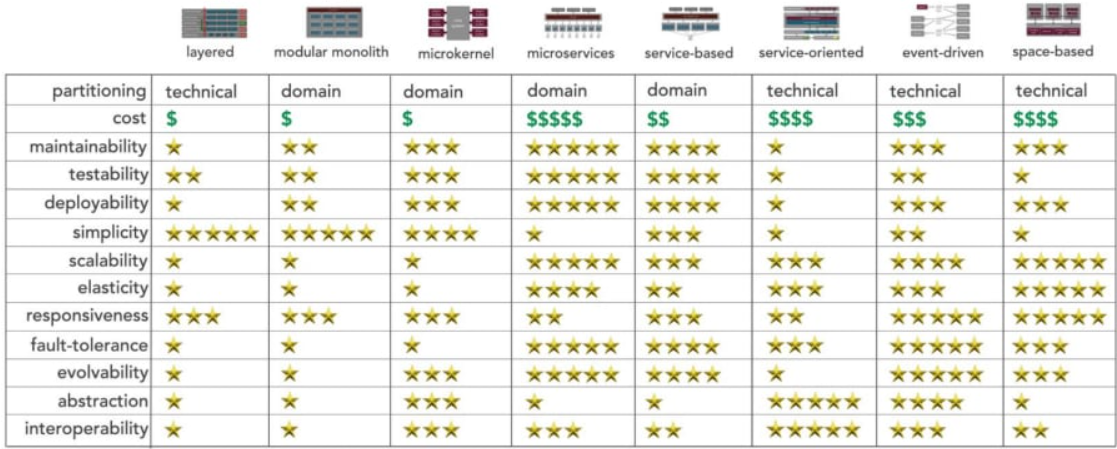
\includegraphics[width=\linewidth]{images/V.Analysis_and_Design/architecture/compare-architecture.png}
\caption{So sánh các đặc tính của các kiểu kiến trúc (Nguồn: Mark Richards, Neal Ford, \textit{Fundamentals of Software Architecture}, O'Reilly, 2nd ed., 2020) \cite{Richards2020FSA}.}
\label{fig:compare-architecture}
\end{figure}


\textbf{C. Phân tích loại trừ:}
Từ biểu đồ trên kết hợp với các yêu cầu nghiệp vụ đã xác định, nhóm tiến hành loại trừ các kiến trúc không phù hợp:
\begin{itemize}
    \item \textbf{Loại bỏ Kiến trúc Vi dịch vụ (Microservices):} 
    \begin{itemize}
        \item \textit{Ưu điểm từ biểu đồ:} Đạt điểm tuyệt đối về khả năng mở rộng (scalability: 5 sao), triển khai độc lập (deployability: 5 sao), và khả năng chịu lỗi (fault-tolerance: 5 sao).
        \item \textit{Nhược điểm nghiêm trọng:} Chi phí vận hành ở mức cao nhất (\$\$\$\$\$) và độ phức tạp có điểm thấp nhất (simplicity: 1 sao). 
        \item \textit{Mâu thuẫn với yêu cầu:} Với nguồn lực hạn chế của đồ án sinh viên, việc vận hành hạ tầng phân tán (service discovery, distributed tracing, container orchestration) là không khả thi. Hơn nữa, các nghiệp vụ mượn/trả sách đòi hỏi cập nhật đồng thời nhiều aggregate (giao dịch, tồn kho, hàng đợi) - nếu tách thành microservices sẽ phải xử lý distributed transactions phức tạp (Saga pattern, 2PC:Two-Phase Commit) với rủi ro eventual consistency.
    \end{itemize}
    
    \item \textbf{Loại bỏ Kiến trúc Phân lớp (Layered) truyền thống:} 
    \begin{itemize}
        \item \textit{Ưu điểm từ biểu đồ:} Đơn giản nhất (simplicity: 5 sao) và chi phí thấp nhất (cost: \$).
        \item \textit{Nhược điểm nghiêm trọng:} Các chỉ số quan trọng cho sự phát triển dài hạn đều ở mức thấp: khả năng bảo trì (maintainability: 1 sao), khả năng kiểm thử (testability: 2 sao), và tính linh hoạt (evolvability: 1 sao).
        \item \textit{Mâu thuẫn với yêu cầu:} Kiến trúc phân lớp theo kỹ thuật (technical layers) dễ dẫn đến tight coupling giữa các logic nghiệp vụ. Đối với hệ thống có yêu cầu tích hợp AI phức tạp (xử lý bất đồng bộ PDF, cập nhật vector embeddings, trigger recommendation engine), kiến trúc này dễ dẫn đến "big ball of mud" với business logic rải rác khắp các layer.
    \end{itemize}

    \item \textbf{Cân nhắc về Kiến trúc Hướng dịch vụ (Service-Based):} 
    \begin{itemize}
        \item \textit{Ưu điểm từ biểu đồ:} Sự cân bằng tốt với hầu hết chỉ số đạt 3--4 sao (maintainability: 4 sao, testability: 4 sao, deployability: 4 sao) và chi phí vừa phải (cost: \$\$).
        \item \textit{Hạn chế trong bối cảnh dự án:} Việc tách ngay từ đầu toàn bộ các nghiệp vụ thư viện thành nhiều service riêng biệt (User Service, Catalog Service, Lending Service, Fine Service) là \textbf{over-engineering} cho giai đoạn MVP. Các service này có phụ thuộc lẫn nhau cao (mượn sách cần kiểm tra user credit score, catalog availability, và fine status) dẫn đến nhiều inter-service calls, tăng network latency và độ phức tạp debugging.
        \item \textit{Kết luận:} Service-Based là hướng đi tương lai hợp lý khi hệ thống cần scale, nhưng chưa phù hợp cho giai đoạn đầu.
    \end{itemize}
\end{itemize}

\textbf{D. Quyết định: Kiến trúc Modular Monolith kết hợp Dịch vụ vệ tinh AI}

Dựa trên phân tích trên, nhóm quyết định áp dụng một cách tiếp cận \textbf{thực dụng và có định hướng phát triển}, kết hợp ưu điểm của Modular Monolith với tính linh hoạt của Service-Based Architecture:

\begin{enumerate}
    \item \textbf{Lõi hệ thống: Modular Monolith (Spring Boot)}
    
    Đây là kiến trúc chủ đạo cho các nghiệp vụ quản lý thư viện (User Management, Catalog, Lending, Fine Management, Engagement).
    
    \textit{Lý do lựa chọn dựa trên biểu đồ so sánh:}
    \begin{itemize}
        \item \textbf{Cân bằng tối ưu:} Modular Monolith cung cấp maintainability (3 sao) và evolvability (3 sao) tốt hơn hẳn Layered Architecture (1 sao) nhưng vẫn giữ được chi phí thấp (cost: \$) và độ đơn giản cao (simplicity: 5 sao).
        \item \textbf{Testability:} Đạt 3 sao - cao hơn đáng kể so với Layered (2 sao) nhờ tách biệt rõ ràng giữa các domain module.
        \item \textbf{Deployability:} Dù chỉ đạt 3 sao (thấp hơn Microservices), nhưng lại phù hợp với nguồn lực đồ án: chỉ cần deploy một artifact duy nhất, không cần orchestration phức tạp.
    \end{itemize}
    
    \textit{Lợi ích nghiệp vụ cụ thể:}
    \begin{itemize}
        \item \textbf{Tính nhất quán giao dịch (ACID):} Các use case phức tạp như trả sách (cần atomic update: trạng thái giao dịch + tính phạt + cập nhật tồn kho + trigger hàng đợi) được đảm bảo trong một transaction duy nhất mà không cần distributed transaction protocols.
        \item \textbf{Tính module hóa cao:} Mặc dù là monolith, code được tổ chức theo \textbf{domain boundaries} (không phải technical layers). Mỗi module (User, Lending, Catalog...) có domain model, use cases, và repositories riêng, giao tiếp thông qua well-defined interfaces. Điều này tạo "exit strategy" - dễ dàng tách module ra thành service riêng trong tương lai nếu cần.
        \item \textbf{DevOps đơn giản:} Chỉ cần một deployment pipeline, một database connection pool, không cần service mesh hay API gateway phức tạp.
    \end{itemize}

    \item \textbf{Dịch vụ vệ tinh: AI Service (Python/FastAPI)}
    
    Mô-đun AI/Recommendation System được tách ra thành một dịch vụ độc lập, giao tiếp với Monolith qua REST API và Message Queue (RabbitMQ).
    
    \textit{Lý do tách riêng:}
    \begin{itemize}
        \item \textbf{Công nghệ khác biệt:} Hệ sinh thái Python (LangChain, HuggingFace Transformers, Sentence-BERT) vượt trội cho ML/NLP so với Java. Việc nhúng Python vào Spring Boot (qua Jython) sẽ gây overhead và mất đi performance của native libraries.
        \item \textbf{Scaling requirements khác biệt:} AI workload (PyMuPDF, vector similarity search, model inference) tiêu tốn CPU/GPU nhiều hơn CRUD nghiệp vụ. Tách riêng cho phép scale độc lập (horizontal scaling với GPU instances) mà không tốn tài nguyên cho monolith.
        \item \textbf{Bất đồng bộ tự nhiên:} Các tác vụ AI (xử lý PDF sau khi thêm sách, cập nhật user embeddings sau khi rating, mượn sách, tương tác) không cần real-time response, có thể chạy background qua message queue. Điều này không block main business flow.
        \item \textbf{Tính module hóa:} AI Service có database riêng (Vector DB: pgvector), không share schema với monolith. Giao tiếp qua API contract rõ ràng, cho phép thay đổi AI stack (model architecture, vector database) mà không ảnh hưởng hệ thống chính.
    \end{itemize}
    
    \textit{Migration path:} Đây là bước đệm hướng tới Service-Based Architecture. Trong tương lai, nếu cần scale, có thể tách dần các module khác (User Service, Notification Service) ra khỏi monolith theo pattern tương tự.
\end{enumerate}


\textbf{E. Đánh giá kiến trúc lai theo các chỉ số:}
Kiến trúc Modular Monolith + AI Satellite này đạt được sự cân bằng tốt nhất cho bối cảnh dự án:
\begin{table}[H]
\centering
\caption{Đánh giá kiến trúc lai so với các chỉ số}
\begin{tabular}{|l|c|l|}
\hline
\textbf{Tiêu chí} & \textbf{Điểm} & \textbf{Nhận xét} \\ \hline
Cost & \$\$ & Giữa Modular Monolith (\$) và Service-Based (\$\$), phù hợp ngân sách \\ \hline
Simplicity & 3-4 sao & Đơn giản hơn Microservices nhưng cần quản lý 2 components \\ \hline
Maintainability & 3-4 sao & Module hóa domain tốt, dễ sửa lỗi và refactor \\ \hline
Testability & 3 sao & Domain logic tách biệt, dễ unit test \\ \hline
Deployability & 2-3 sao & Deploy 2 artifacts (Monolith + AI), CI/CD đơn giản \\ \hline
Scalability & 3 sao & AI service scale độc lập, monolith scale theo nhu cầu \\ \hline
Evolvability & 4 sao & Có thể tách dần modules ra thành services khi cần \\ \hline
\end{tabular}
\end{table}

\textbf{Kết luận:} Kiến trúc Modular Monolith + AI Satellite Service đạt được ba mục tiêu then chốt: (1) Đảm bảo tính nhất quán giao dịch cho nghiệp vụ core, (2) Tối ưu hóa AI workload với công nghệ và scaling phù hợp, (3) Giữ độ phức tạp và chi phí ở mức chấp nhận được cho đồ án, đồng thời tạo nền tảng để mở rộng thành Service-Based Architecture hoặc Microservice Architecture trong tương lai.


\subsection{Thiết kế cơ sở dữ liệu}
\label{subsec:database-design}

Thiết kế cơ sở dữ liệu là quá trình chuyển đổi từ mô hình phân tích yêu cầu và các thực thể đã được đặc tả ở các phần trước thành một cấu trúc lưu trữ logic và vật lý. Mục tiêu là xây dựng một nền tảng dữ liệu nhất quán, toàn vẹn, hiệu quả và có khả năng mở rộng để hỗ trợ toàn bộ nghiệp vụ của hệ thống, từ các giao dịch mượn trả cơ bản đến các tính năng AI phức tạp.

\subsubsection{Lựa chọn Hệ Quản trị Cơ sở dữ liệu (HQTCSDL)}
Dựa trên bản chất quan hệ chặt chẽ của dữ liệu (người dùng, sách, lượt mượn), hệ thống lựa chọn \textbf{PostgreSQL} làm HQTCSDL chính.
\begin{itemize}
 \item \textbf{Tính tin cậy và toàn vẹn dữ liệu:} PostgreSQL nổi tiếng với sự tuân thủ nghiêm ngặt các tiêu chuẩn ACID (Atomicity, Consistency, Isolation, Durability), đảm bảo các giao dịch nghiệp vụ quan trọng như mượn, trả, và tính phí phạt luôn được thực hiện một cách an toàn.
 \item \textbf{Hỗ trợ các kiểu dữ liệu nâng cao:} PostgreSQL hỗ trợ các kiểu dữ liệu phức tạp như JSONB, rất hữu ích để lưu trữ các metadata linh hoạt. Đặc biệt, thông qua các extension như \texttt{pgvector}, nó có khả năng lưu trữ và truy vấn các vector embedding hiệu quả, phục vụ trực tiếp cho tính năng tìm kiếm ngữ nghĩa.
 \item \textbf{Khả năng mở rộng:} Đây là một hệ quản trị CSDL mã nguồn mở mạnh mẽ, đã được chứng minh về hiệu năng trong các hệ thống quy mô lớn.
\end{itemize}

\subsubsection{Mô hình Quan hệ Thực thể (ERD)}
Bên dưới là sơ đồ ERD tổng quan của toàn bộ hệ thống.

\begin{figure}[htbp]
 \centering
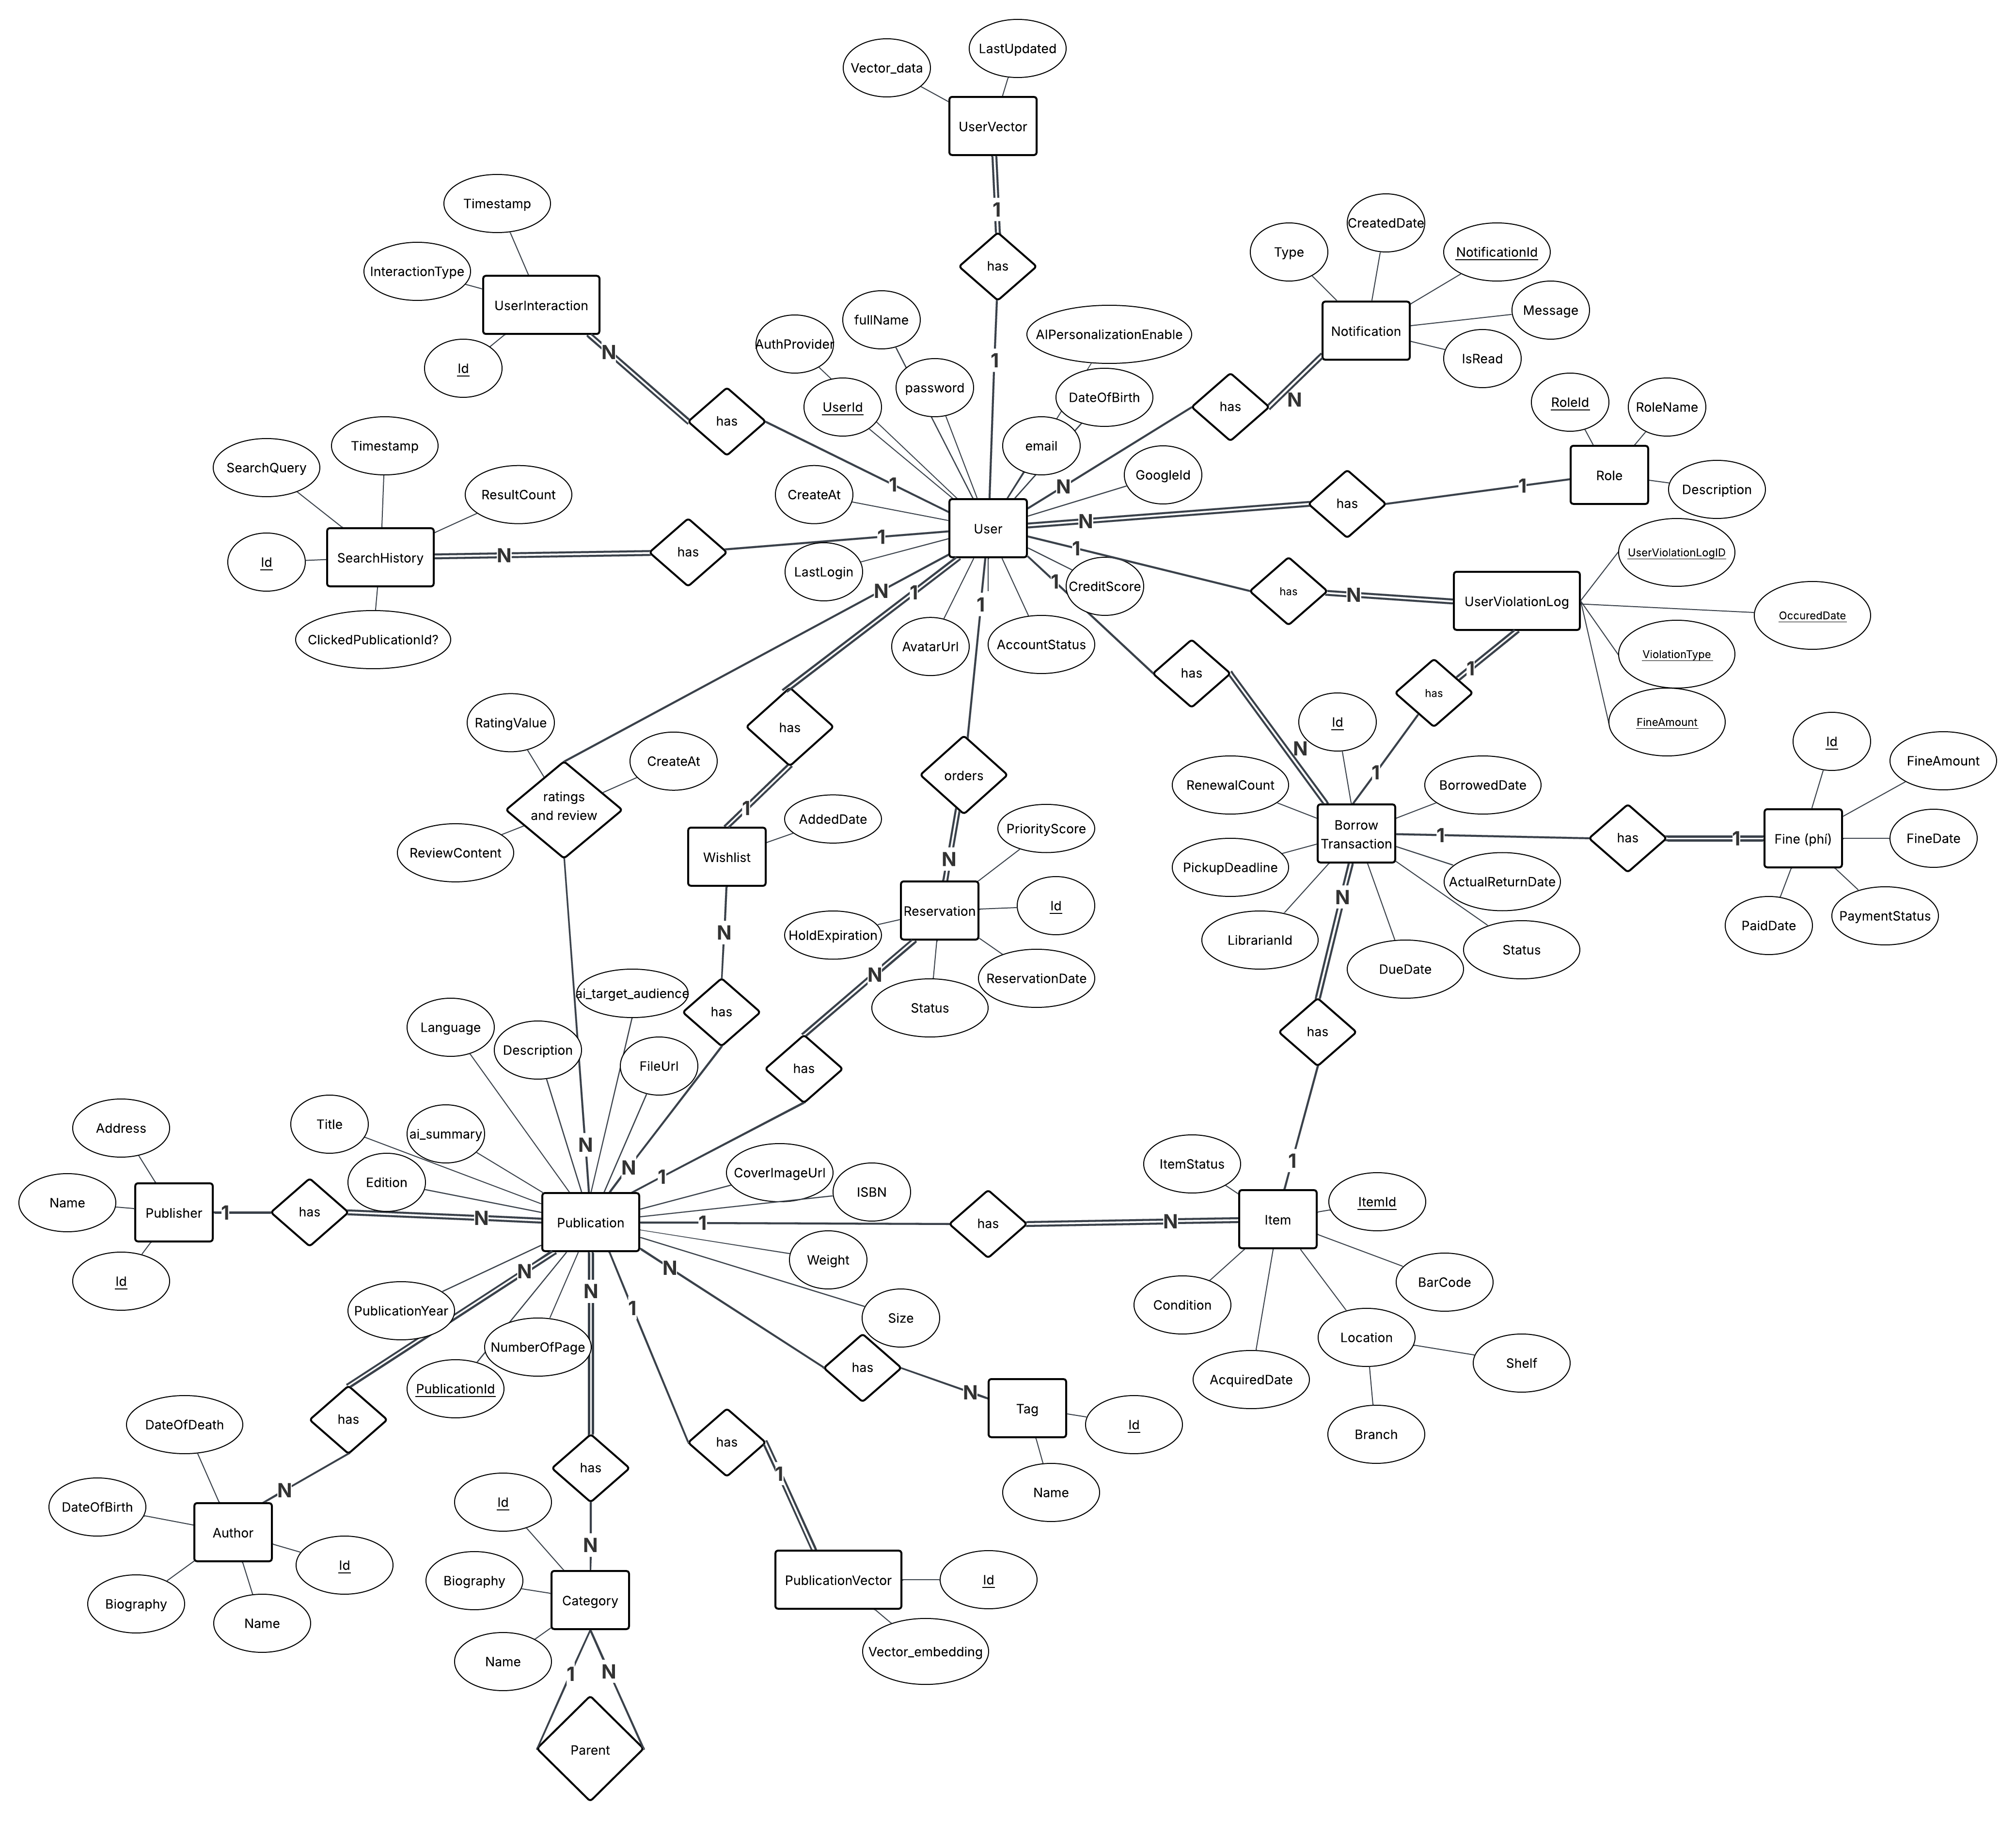
\includegraphics[width=1\linewidth]{images//V.Analysis_and_Design/ERD.png}
 \caption{Sơ đồ Quan hệ Thực thể (ERD) tổng thể của hệ thống}
 \label{fig:erd}
\end{figure}
\FloatBarrier

\subsubsection{Ánh xạ lược đồ cơ sở dữ liệu quan hệ}
Sau khi thực hiện quá trình ánh xạ từ mô hình ERD ở trên, ta thu được một lược đồ cơ sở dữ liệu quan hệ như trình bày bên dưới. Trong lược đồ này, các thuộc tính chi tiết đã được lược bớt nhằm tập trung làm rõ mối quan hệ giữa các bảng trong hệ thống.

\begin{figure}[htbp]
 \centering
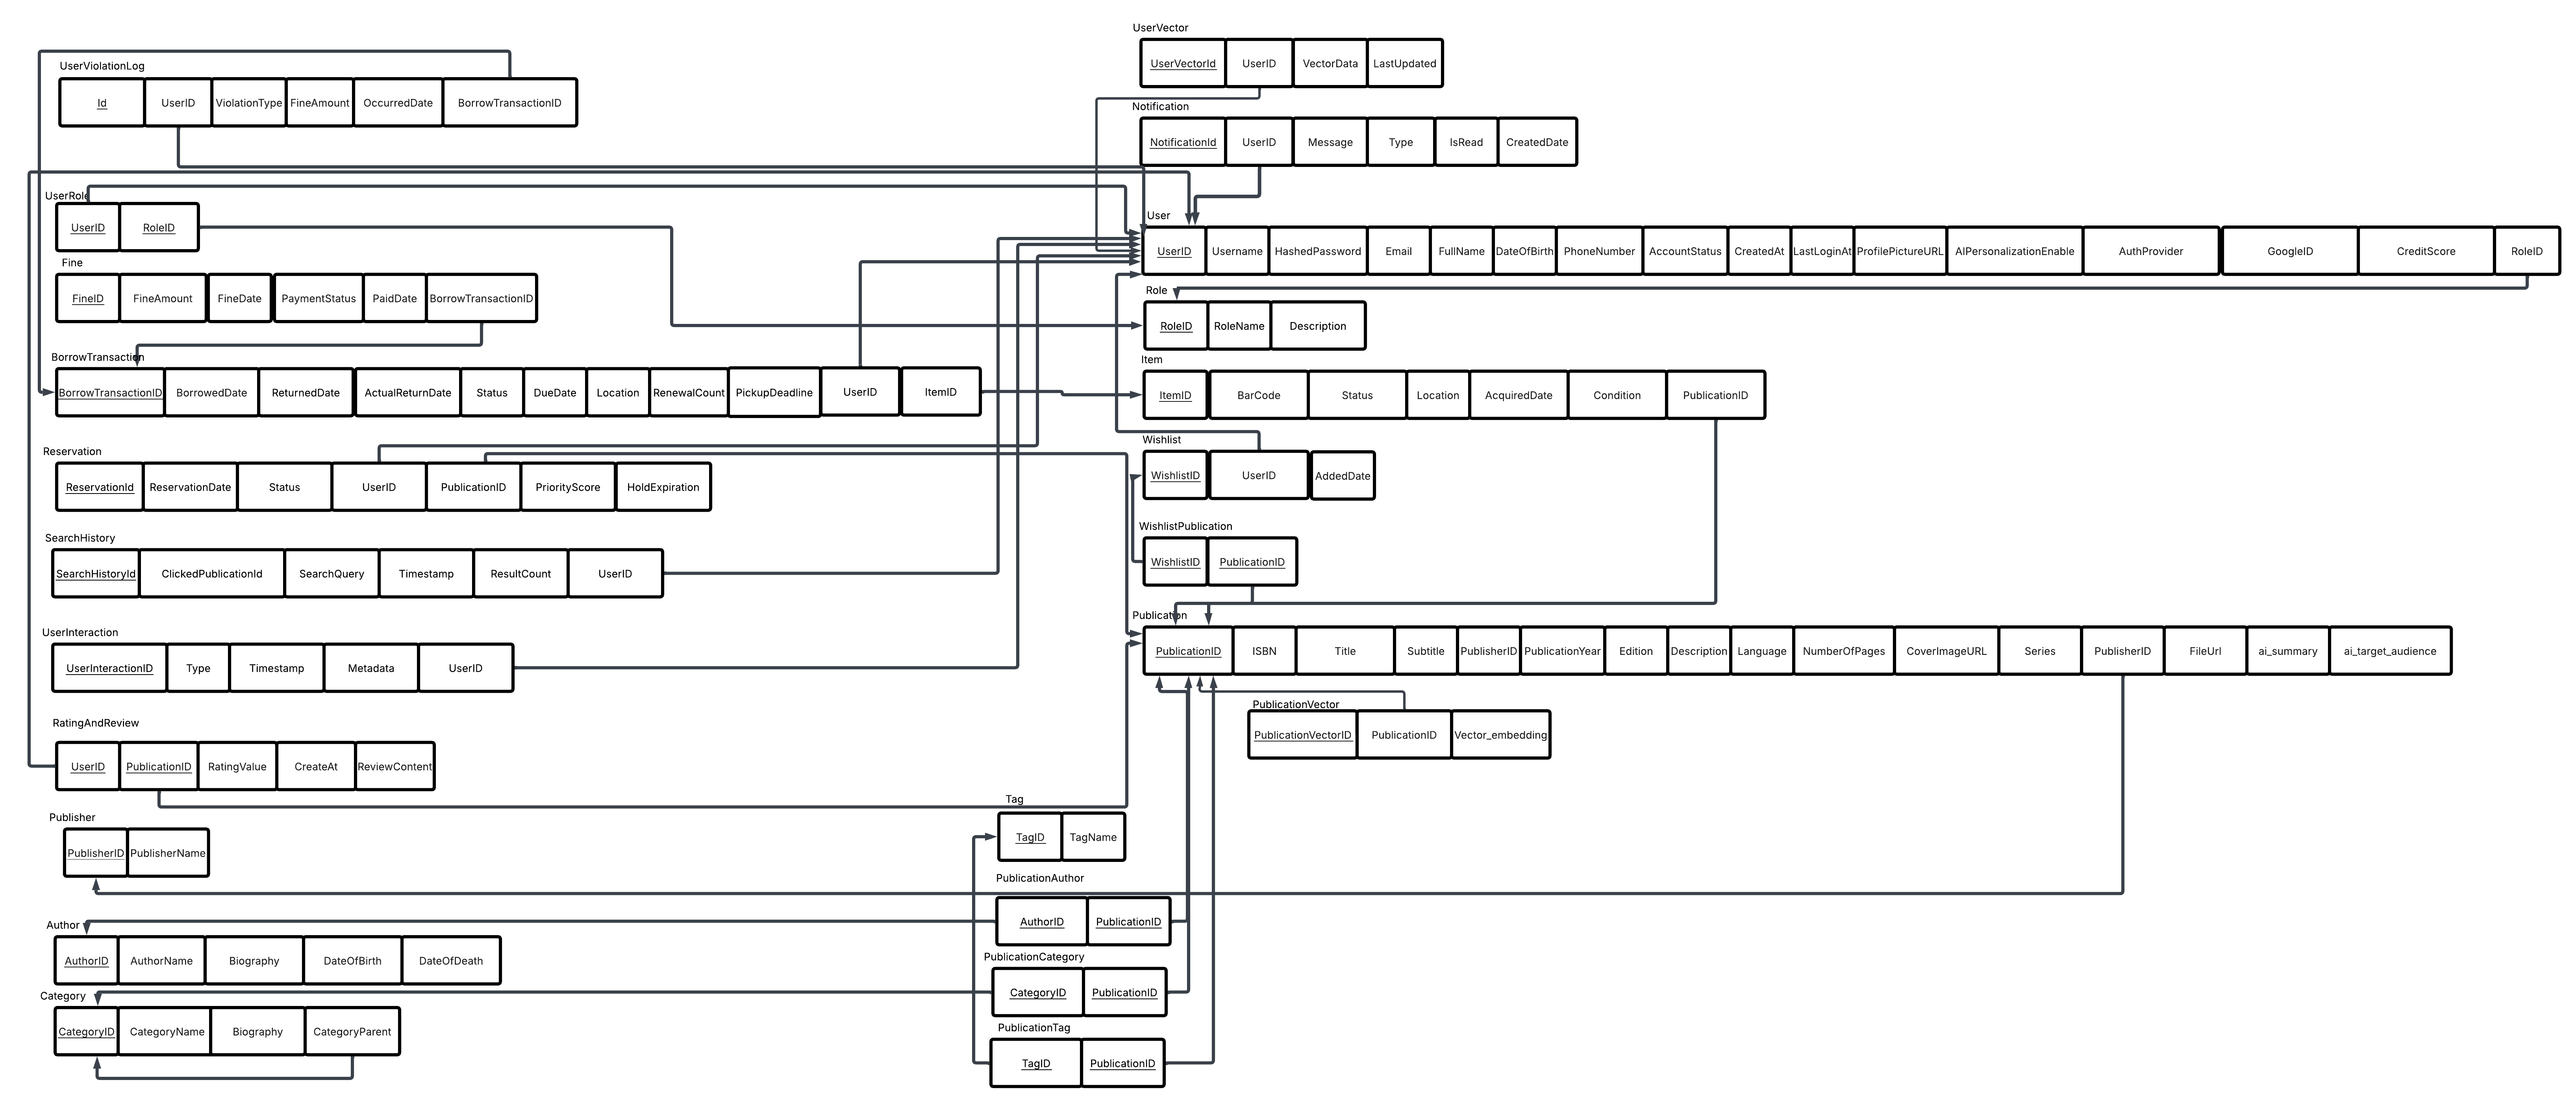
\includegraphics[width=1\linewidth]{images//V.Analysis_and_Design/Mapping.png}
 \caption{Ánh xạ cơ sở dữ liệu quan hệ ở dạng tổng quát}
 \label{fig:mapping}
\end{figure}
\FloatBarrier

\subsection{Thiết kế chi tiết bên trong}
\subsubsection{Mô hình kiến trúc chi tiết}
Sau khi quyết định sử dụng kiến trúc Modular Monolith kết hợp AI Satellite Service, phần này trình bày chi tiết cấu trúc nội bộ của từng thành phần và các nguyên tắc thiết kế được áp dụng.

\textbf{A. Tổng quan kiến trúc hệ thống:}
\begin{figure}[htbp]
 \centering
 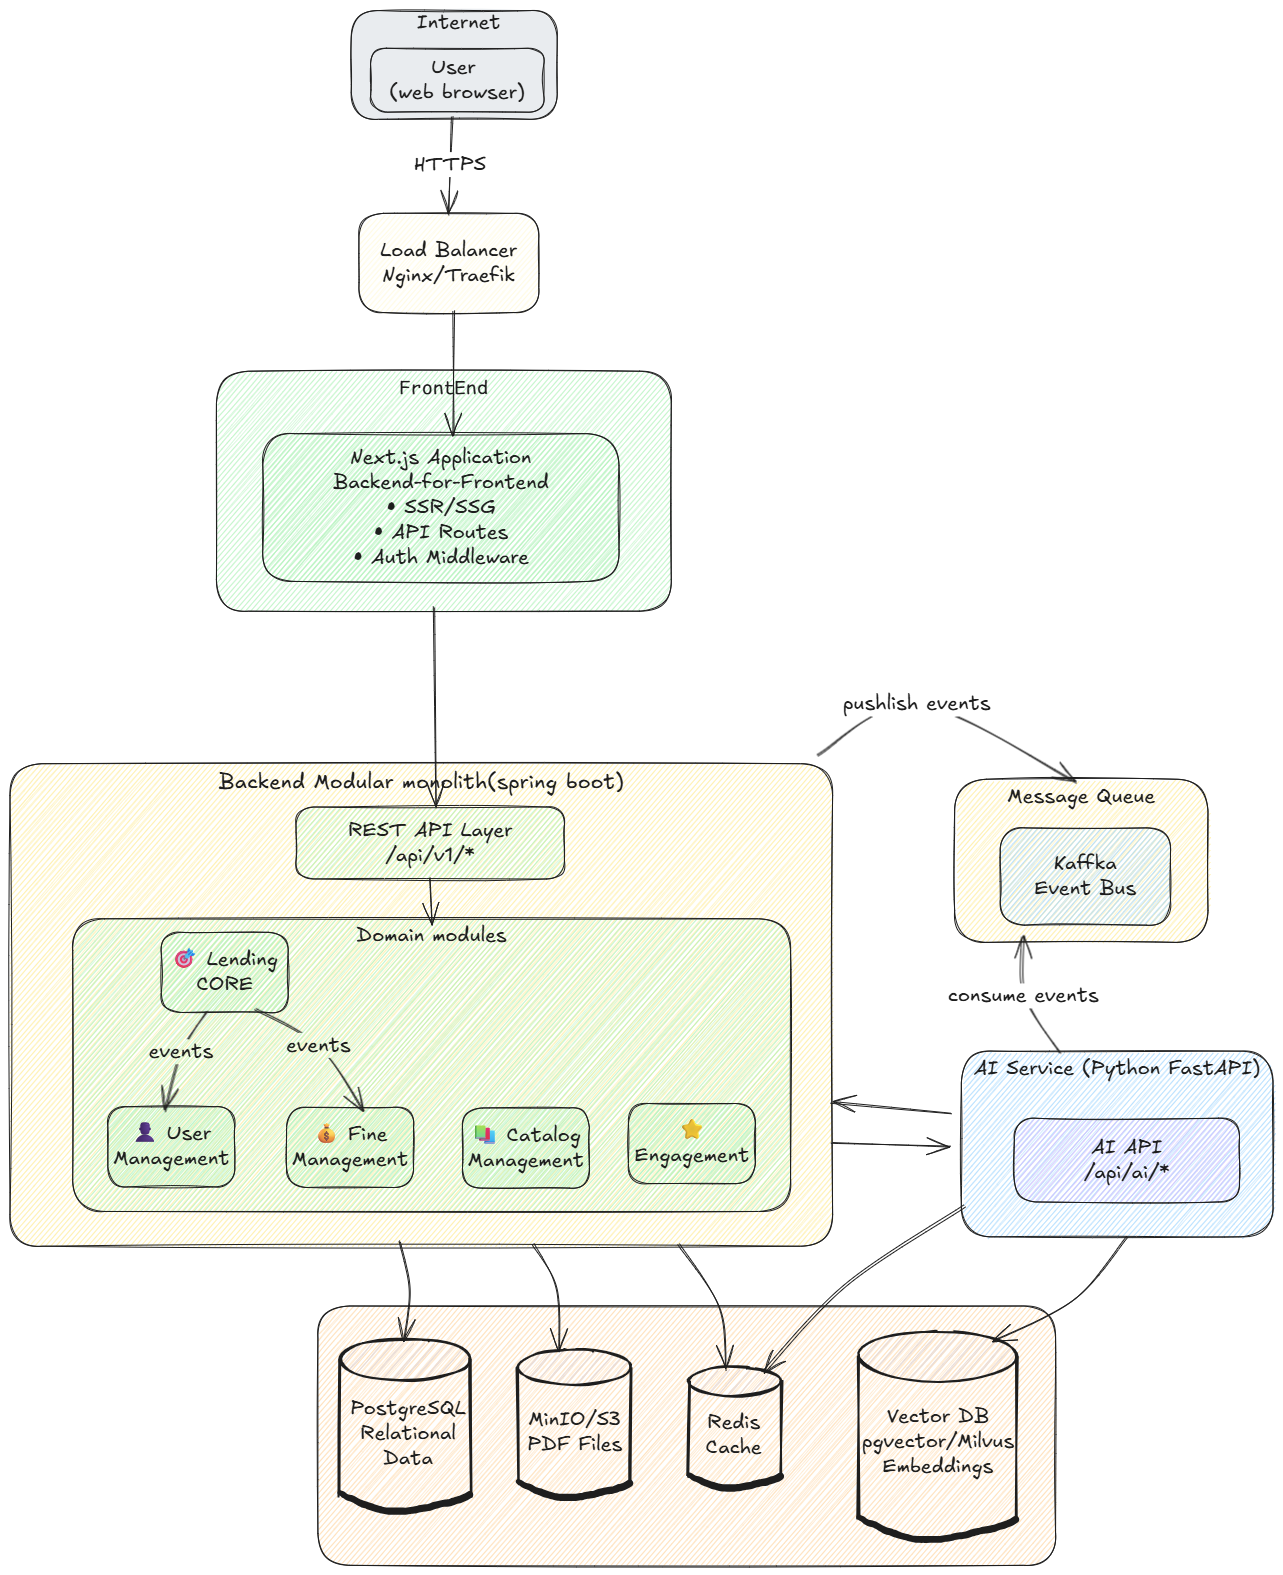
\includegraphics[width=1\linewidth]{images/V.Analysis_and_Design/architecture/system_architecture_overview.png}
 \caption{Sơ đồ kiến trúc tổng thể hệ thống}
 \label{fig:system_architecture_overview}
\end{figure}
Hệ thống bao gồm ba thành phần chính:
\begin{enumerate}
    \item \textbf{Frontend (Next.js):} Giao diện người dùng đóng vai trò Backend-for-Frontend (BFF), xử lý SSR và tổng hợp API calls.
    \item \textbf{Backend Monolith (Spring Boot):} Lõi nghiệp vụ áp dụng Domain-Driven Design và Clean Architecture.
    \item \textbf{AI Service (Python FastAPI):} Dịch vụ độc lập xử lý các tác vụ Machine Learning và Vector Search.
\end{enumerate}


\textbf{B.1). Kiến trúc Backend Monolith (Spring Boot)}
\textbf{Tổ chức theo Bounded Contexts (DDD):}

Thay vì tổ chức code theo các lớp kỹ thuật ngang (technical layers), hệ thống được chia thành các module theo ranh giới nghiệp vụ (domain boundaries), mỗi module tương ứng với một Bounded Context trong Domain-Driven Design:

\begin{figure}[htbp]
 \centering
 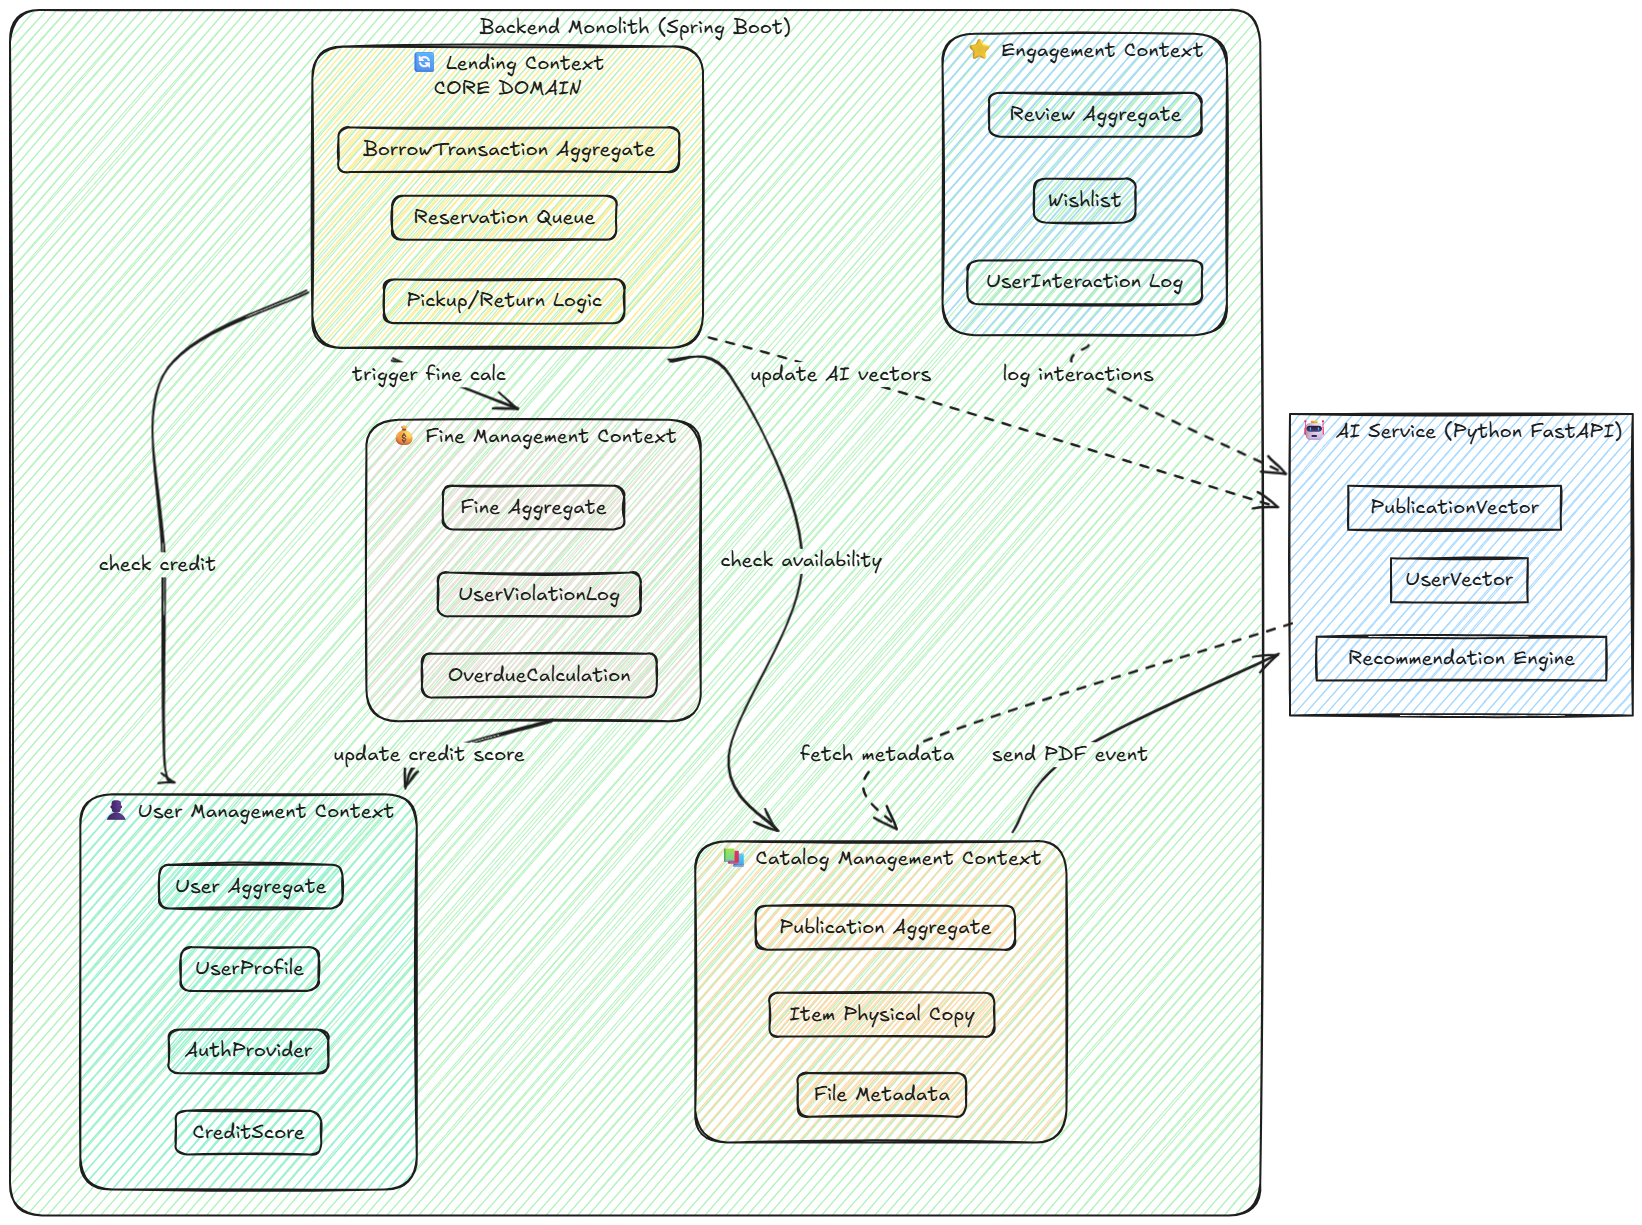
\includegraphics[width=1\linewidth]{images/V.Analysis_and_Design/architecture/bounded_contexts.png}
 \caption{Các Bounded Contexts trong hệ thống}
 \label{fig:bounded_contexts}
\end{figure}

\begin{itemize}
    \item \textbf{User Management Context:} Quản lý người dùng, xác thực (Local + Google OAuth), phân quyền, và credit scoring.
    \item \textbf{Catalog Management Context:} Quản lý thông tin xuất bản phẩm (Publication), các bản sao vật lý (Item), metadata sách, và file storage.
    \item \textbf{Lending Context:} \textit{(Core Domain)} - Quản lý vòng đời mượn/trả sách (BorrowTransaction), hàng đợi đặt chỗ (Reservation), và các business rules phức tạp về deadline, pickup, renewal.
    \item \textbf{Fine Management Context:} Quản lý tiền phạt, vi phạm người dùng (UserViolationLog), tính toán credit score.
    \item \textbf{Engagement Context:} Quản lý đánh giá sách (Review), danh sách yêu thích (Wishlist), và log tương tác người dùng (UserInteraction).
\end{itemize}

Mỗi Bounded Context được thiết kế như một "mini-service" bên trong monolith, có thể tách ra thành service độc lập trong tương lai mà không cần refactor lớn.

\textbf{Clean Architecture bên trong mỗi Module:}

Bên trong mỗi Bounded Context, code được tổ chức theo 4 layers của Clean Architecture để đảm bảo tách biệt trách nhiệm và independence từ framework/database:
\begin{figure}[htbp]
 \centering
 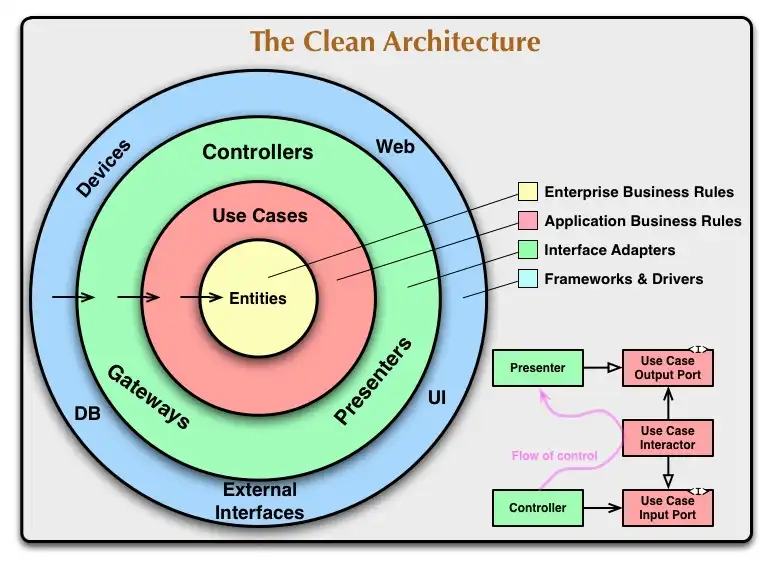
\includegraphics[width=1\linewidth]{images/V.Analysis_and_Design/architecture/clean-architecture.png}
 \caption{Clean architecture (R. C. Martin, \textit{Clean Architecture: A Craftsman’s Guide to Software Structure and Design},  Pearson Education, 2018 \cite{martin2018clean})}
 \label{fig:clean_architecture_layers}
\end{figure}
\begin{figure}[htbp]
 \centering
 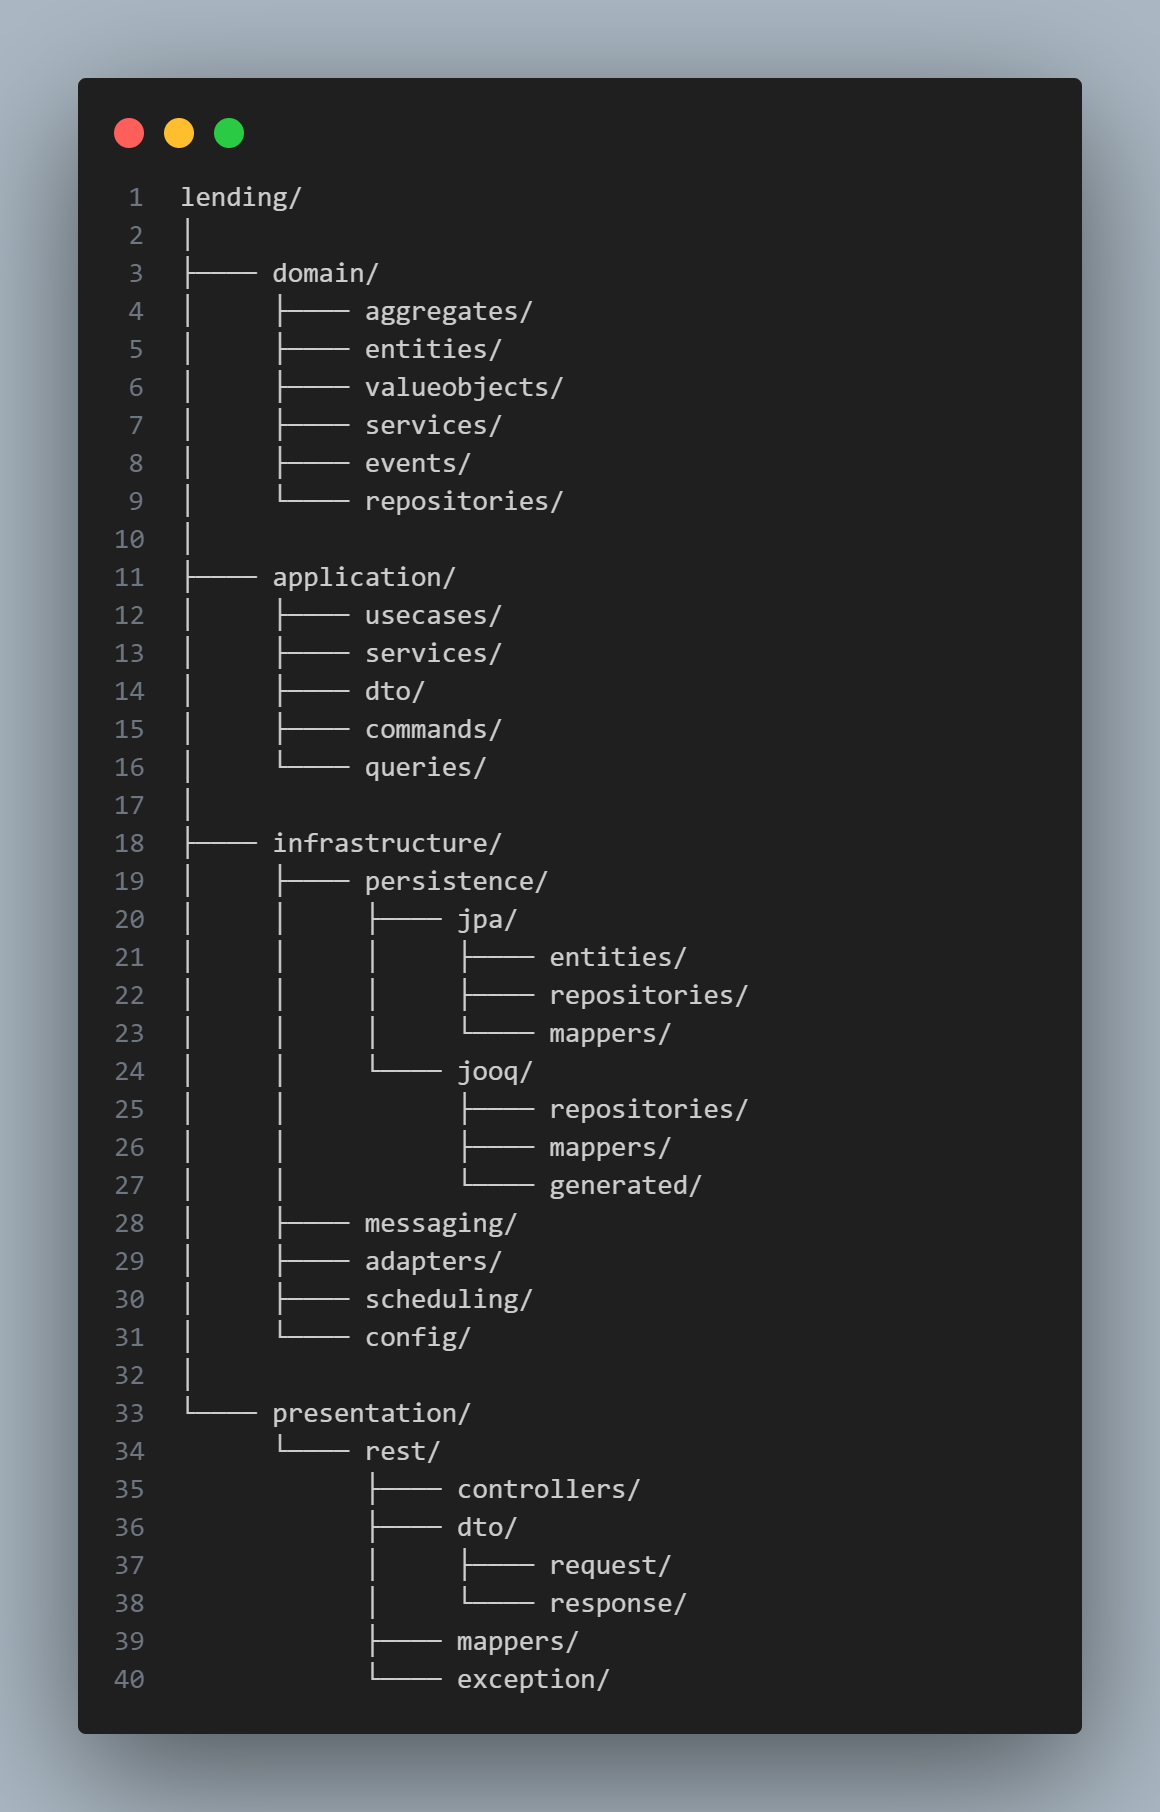
\includegraphics[width=0.8\linewidth]{images/V.Analysis_and_Design/architecture/folder_structure_backend.png}
 \caption{Cấu trúc Clean Architecture kết hợp Domain-Driven Design trong một Module}
 \label{fig:clean_architecture_in_module}
\end{figure}

\textbf{1. Domain Layer (Lõi nghiệp vụ - Innermost):}
\begin{itemize}
    \item \textbf{Entities và Aggregates:} Chứa các đối tượng nghiệp vụ cốt lõi với business invariants. Ví dụ:
    \begin{itemize}
        \item \texttt{BorrowTransaction} Aggregate: Đảm bảo các quy tắc như "không được pickup sau 24h", "tối đa gia hạn 2 lần", "phải kiểm tra hư hại khi trả".
        \item \texttt{Publication} Aggregate: Đảm bảo "ít nhất một Item để có thể cho mượn", "ISBN không trùng".
        \item \texttt{User} Aggregate: Đảm bảo "credit score >= 0", "không mượn quá 5 cuốn cùng lúc".
    \end{itemize}
    
    \item \textbf{Value Objects:} Các đối tượng bất biến đại diện cho khái niệm nghiệp vụ không có identity riêng (ví dụ: \texttt{ISBN}, \texttt{DateRange}, \texttt{Address}).
    
    \item \textbf{Domain Services:} Logic nghiệp vụ không thuộc về một Entity/Aggregate cụ thể. Ví dụ:
    \begin{itemize}
        \item \texttt{OverdueCalculationService}: Tính tiền phạt dựa trên số ngày trễ và chính sách thư viện.
        \item \texttt{PriorityQueueService}: Tính điểm ưu tiên cho hàng đợi đặt chỗ.
    \end{itemize}
    
    \item \textbf{Domain Events:} Biểu diễn các sự kiện nghiệp vụ quan trọng để các module khác có thể phản ứng (loose coupling):
    \begin{itemize}
        \item \texttt{BookBorrowedEvent}, \texttt{BookReturnedEvent}
        \item \texttt{FineIncurredEvent}, \texttt{UserBannedEvent}
        \item \texttt{ReservationExpiredEvent}, \texttt{AIProcessingCompletedEvent}
    \end{itemize}
    
    \item \textbf{Repository Interfaces:} Domain định nghĩa các interface (contract) mà Infrastructure sẽ implement. Domain không quan tâm dùng JPA, JDBC hay MongoDB.
    
    \item \textbf{Ràng buộc nghiêm ngặt:} Domain Layer KHÔNG ĐƯỢC phụ thuộc vào bất kỳ layer nào khác, không import Spring annotations, không biết HTTP hay Database. Đây là "business logic in pure Java".
\end{itemize}

\textbf{2. Application Layer (Use Cases - Orchestrator):}
\begin{itemize}
    \item \textbf{Use Case Services:} Mỗi use case là một entry point cho một chức năng nghiệp vụ hoàn chỉnh. Ví dụ:
    \begin{itemize}
        \item \texttt{BorrowBookUseCase}: Điều phối luồng mượn sách (validate user → check availability → create transaction → publish event).
        \item \texttt{ReturnBookUseCase}: Điều phối luồng trả sách (update transaction → check damage → calculate fine → trigger queue → notify AI).
        \item \texttt{ProcessReservationQueueUseCase}: Xử lý hàng đợi (find next user → notify → set hold expiration).
    \end{itemize}
    
    \item \textbf{Trách nhiệm chính:}
    \begin{itemize}
        \item Orchestrate workflow: Gọi repositories để load aggregates, gọi domain services, và save kết quả.
        \item Quản lý transaction boundaries (sử dụng \texttt{@Transactional} annotation của Spring).
        \item Publish domain events sau khi transaction commit thành công.
        \item Transform exceptions: Chuyển domain exceptions thành application-level error codes.
    \end{itemize}
    
    \item \textbf{Application Services:} Các facade cho phép module khác gọi vào (public API giữa các modules).
    
    \item \textbf{DTOs (Data Transfer Objects):} Chuyển đổi giữa domain objects và external representations (JSON, DTO cho API).
    
    \item \textbf{Lưu ý:} Application Layer được phép phụ thuộc vào Domain Layer và định nghĩa interfaces cho Infrastructure (Dependency Inversion Principle).
\end{itemize}


\textbf{3. Infrastructure Layer (Technical Implementation - Outermost):}
\begin{itemize}
    \item \textbf{Repository Implementations:} Hiện thực các repository interfaces từ Domain bằng JPA/Hibernate, JDBC, hoặc bất kỳ persistence technology nào. Ví dụ:
    \begin{itemize}
        \item \texttt{BorrowTransactionRepositoryJpa}: Implements \texttt{BorrowTransactionRepository} interface.
        \item Mapping giữa Domain Aggregate (\texttt{BorrowTransaction}) và JPA Entity (\texttt{BorrowTransactionJpaEntity}).
    \end{itemize}
    
    \item \textbf{External Service Adapters:} Tích hợp với các dịch vụ bên ngoài:
    \begin{itemize}
        \item Email/SMS Service (gửi notification)
        \item File Storage (MinIO/S3 để lưu PDF sách)
        \item Payment Gateway (thanh toán phạt trực tuyến)
        \item OAuth Provider (Google Authentication)
    \end{itemize}
    
    \item \textbf{Event Infrastructure:} Hiện thực event publishing/subscribing:
    \begin{itemize}
        \item In-memory event bus (Spring ApplicationEventPublisher) cho giao tiếp nội bộ giữa các modules.
        \item Message Queue client (RabbitMQ) cho giao tiếp với AI Service.
    \end{itemize}
    
    \item \textbf{Technical Services:}
    \begin{itemize}
        \item Scheduler (Spring \texttt{@Scheduled}) cho background jobs (check overdue daily).
        \item Caching (Redis/Caffeine) cho frequently accessed data.
        \item Security (JWT token generation/validation, password hashing).
    \end{itemize}
    
    \item \textbf{Configuration:} Database connection pools, message queue configuration, security settings.
\end{itemize}


\textbf{4. Presentation Layer (Interface Adapters):}
\begin{itemize}
    \item \textbf{REST Controllers:} Expose các use cases qua HTTP/REST API. Mỗi Bounded Context có controller riêng:
    \begin{itemize}
        \item \texttt{UserController} (\texttt{/api/v1/users/*})
        \item \texttt{LendingController} (\texttt{/api/v1/lending/*})
        \item \texttt{CatalogController} (\texttt{/api/v1/books/*})
    \end{itemize}
    
    \item \textbf{Trách nhiệm:}
    \begin{itemize}
        \item Nhận HTTP requests, validate syntax (JSON format, required fields, regex).
        \item Chuyển đổi Request DTOs → Commands/Queries cho Application Layer.
        \item Authentication \& Authorization: Extract user info từ JWT, check permissions.
        \item Chuyển đổi kết quả từ Application Layer → HTTP Response (JSON).
        \item Error handling: Chuyển exceptions thành HTTP status codes (400, 401, 403, 404, 500).
    \end{itemize}
    
    \item \textbf{Nguyên tắc:} Controllers phải "thin" - chỉ làm việc chuyển đổi và delegation, KHÔNG chứa business logic.
\end{itemize}

\textbf{Dependency Rule (Nguyên tắc phụ thuộc):}
Clean Architecture tuân thủ nguyên tắc: \textbf{Dependencies chỉ được point inward} (từ ngoài vào trong):

\begin{center}
\texttt{Presentation → Application → Domain ← Infrastructure}
\end{center}

\begin{itemize}
    \item Domain Layer: Không phụ thuộc vào ai (pure business logic).
    \item Application Layer: Chỉ phụ thuộc Domain, định nghĩa interfaces cho Infrastructure.
    \item Infrastructure \& Presentation: Phụ thuộc cả Domain và Application, implement interfaces.
\end{itemize}

Điều này đảm bảo business logic (Domain) không bị "ô nhiễm" bởi framework, database hay HTTP concerns.


%-----------------------------AI-----------------------------------


\textbf{B. Kiến trúc AI Service (Python FastAPI)}
Hệ thống AI Service được thiết kế như một \textit{Dịch vụ Vệ tinh Độc lập} (Autonomous Satellite Microservice), tách biệt hoàn toàn khỏi khối Monolith (Spring Boot). Quyết định này nhằm tận dụng sức mạnh của hệ sinh thái Python trong các tác vụ Học máy (Machine Learning) và Xử lý ngôn ngữ tự nhiên (NLP), đồng thời đảm bảo khả năng mở rộng độc lập cho các tác vụ tính toán nặng.
\textbf{B.1. Chiến lược thiết kế và Lựa chọn công nghệ}
Khác với Backend chính tập trung vào tính toàn vẹn dữ liệu giao dịch, AI Service tập trung vào hiệu năng tính toán ma trận và xử lý bất đồng bộ.
\begin{itemize}
\item \textbf{Web Framework - FastAPI:} Được lựa chọn thay vì Flask/Django nhờ khả năng xử lý bất đồng bộ (Native Async/Await) vượt trội, cho phép phục vụ hàng nghìn yêu cầu suy luận (inference) đồng thời mà không bị tắc nghẽn I/O. Tích hợp sẵn Pydantic giúp kiểm soát chặt chẽ kiểu dữ liệu đầu vào cho các mô hình ML.
\item \textbf{Kiến trúc Phi trạng thái (Stateless):} AI Service không lưu trữ session người dùng. Mọi trạng thái cần thiết được truyền qua payload của request hoặc truy xuất từ Database/Cache, giúp dễ dàng mở rộng theo chiều ngang (Horizontal Scaling) bằng cách tăng số lượng container.
\end{itemize}
\textbf{B.2. Cấu trúc Phân tầng (Layered Architecture)} \\ 
Kiến trúc nội bộ của AI Service được tinh gọn thành 3 tầng chính để tối ưu hóa đường đi của dữ liệu: \\
\textbf{a. API Layer (Giao tiếp \& Định tuyến):}
\begin{itemize}
\item \textit{Semantic Search Router:} \texttt{POST /api/v1/search/semantic}
\begin{itemize}
\item Xử lý truy vấn tìm kiếm bằng ngôn ngữ tự nhiên.
\item Pipeline: Tiền xử lý text $\rightarrow$ Encoding $\rightarrow$ Vector Search.
\end{itemize}
\item \textit{Recommendation Router:} \texttt{GET /api/v1/recommendations/\{user\_id\}}
\begin{itemize}
\item Trả về danh sách gợi ý cá nhân hóa dựa trên ngữ cảnh (Trang chủ, Chi tiết sách).
\end{itemize}
\item \textit{Data Ingestion Router:} \texttt{POST /api/v1/ingest/pdf}
\begin{itemize}
\item Endpoint bất đồng bộ (Async) để nhận yêu cầu xử lý tài liệu mới (OCR, Embedding).
\end{itemize}
\end{itemize}
\textbf{b. Service Layer (Logic nghiệp vụ ML):}
Đây là trái tim của hệ thống, chứa các pipeline xử lý dữ liệu phức tạp:
\begin{itemize}
\item \textbf{Embedding Service:} Sử dụng mô hình \texttt{bkai-foundation-models/vietnamese-bi-encoder} (SBERT) để chuyển đổi văn bản tiếng Việt thành các vector 768 chiều. Mô hình này được huấn luyện trên tập dữ liệu pháp lý Zalo Legal, giúp hiểu tốt văn phong học thuật.
\item \textbf{PDF Processing Pipeline:}
\begin{itemize}
\item \textit{Extraction:} Sử dụng \textbf{PyMuPDF} để trích xuất văn bản tốc độ cao (nhanh hơn 10x so với pypdf).
\item \textit{Chunking:} Áp dụng chiến lược Cửa sổ trượt (Sliding Window) với kích thước chunk 256 tokens và độ chồng lấn (overlap) 50 tokens để bảo toàn ngữ cảnh giữa các đoạn cắt.
\item \textit{OCR Fallback:} Tích hợp \textbf{Tesseract} để xử lý các tài liệu dạng scan khi PyMuPDF không tìm thấy lớp văn bản.
\end{itemize}
\item \textbf{Recommendation Engine:} Sử dụng thư viện \textbf{LightFM} để cài đặt thuật toán Lai ghép (Hybrid), kết hợp giữa Lọc cộng tác (Collaborative Filtering) và Lọc nội dung (Content-based).
\end{itemize}
\textbf{c. Data \& Storage Layer:}
\begin{itemize}
\item \textbf{Vector Database (PostgreSQL + pgvector):} Lưu trữ embeddings của sách và người dùng. Sử dụng chỉ mục \textbf{HNSW} (Hierarchical Navigable Small World) để tối ưu hóa tốc độ tìm kiếm láng giềng gần nhất (ANN) thay vì quét toàn bộ bảng (IVFFlat).
\item \textbf{Model Store:} Các mô hình nặng (SBERT) được tải sẵn vào RAM khi khởi động (Pre-loaded) để giảm độ trễ (Latency).
\item \textbf{Cache (Redis):} Lưu trữ kết quả của các truy vấn phổ biến và vector người dùng (User Vectors) để giảm tải tính toán lại.
\end{itemize}


\begin{figure}[htbp]
\centering
\resizebox{\textwidth}{!}{%
    \begin{tikzpicture}[
      node distance=2.5cm and 2cm, % TĂNG MẠNH khoảng cách (Dọc 2.5, Ngang 2)
      auto,
      % --- STYLES (Giữ nguyên nhưng tinh chỉnh font) ---
      user/.style={
        rectangle, draw, rounded corners,
        minimum width=2.5cm, minimum height=1.2cm,
        fill=blue!5, align=center, font=\normalsize
      },
      service/.style={
        rectangle, draw, rounded corners,
        minimum width=3.5cm, minimum height=1.5cm, % Cho node to ra
        fill=gray!10, align=center, font=\normalsize
      },
      db/.style={
        cylinder, shape border rotate=90,
        draw, minimum height=1.5cm,
        minimum width=2cm, align=center,
        fill=orange!10, font=\small, aspect=0.25
      },
      queue/.style={
        rectangle, draw, dashed,
        minimum width=3cm, minimum height=1.2cm,
        fill=red!5, align=center, font=\normalsize
      },
      sync_arrow/.style={
        ->, thick, draw=blue!70, >=stealth
      },
      async_arrow/.style={
        ->, thick, dashed, draw=red!70, >=stealth
      },
      label_text/.style={
        font=\small, align=center, auto=false, fill=white, inner sep=1pt % Thêm nền trắng cho chữ để không bị dòng kẻ cắt qua
      }
    ]

    % --- 1. NODES (KHỐI) ---
    
    % Main Flow
    \node[user] (user) {User\\(Browser)};
    \node[service, right=of user] (frontend) {Frontend\\(Next.js)};
    \node[service, right=of frontend] (backend) {Core Backend\\(Spring Boot)};

    % AI Service: Đẩy xuống thật sâu (5cm) để khoảng giữa cực rộng
    \node[service, below=5cm of backend, fill=green!5, draw=green!60!black] (ai_api) {AI Service API\\(FastAPI)};
    \node[service, below=0.8cm of ai_api, fill=green!5, draw=green!60!black] (ai_worker) {Celery Workers\\(OCR/Embed)};
    
    % Group AI
    \node[fit=(ai_api)(ai_worker), draw=green!60!black, dashed, inner sep=0.5cm, label={[green!60!black]above left:\textbf{AI Microservice}}] (ai_group) {};

    % RabbitMQ: Treo lơ lửng ở giữa khoảng trống mênh mông đó
    \node[queue, right=of backend, xshift=0.5cm, yshift=-2.5cm] (rabbitmq) {Message Queue\\(RabbitMQ)};

    % Database Column: Đẩy xa tít sang phải (xshift=4.5cm)
    \node[db, right=of ai_api, xshift=4.5cm] (pgvector) {Vector DB\\(pgvector)};
    
    % Giãn khoảng cách giữa các DB (2.5cm)
    \node[db, above=2.5cm of pgvector] (redis) {Redis Cache}; 
    \node[db, below=2.5cm of pgvector] (minio) {File Storage\\(MinIO/S3)};

    % --- 2. EDGES (KẾT NỐI) ---

    % Sync Flow (Xanh)
    \draw[sync_arrow] (user) -- node[below] {HTTP} (frontend);
    \draw[sync_arrow] (frontend) -- (backend);
    
    % Backend -> AI API
    \draw[sync_arrow] (backend) to[bend right=40] node[left, label_text, pos=0.5, xshift=-0.3cm] {1. Search/Rec Req} (ai_api);
    
    % AI API -> VectorDB
    \draw[sync_arrow] (ai_api) -- node[above, label_text] {2. Query} (pgvector);
    
    % AI API -> Redis (Cache)
    \draw[sync_arrow] (ai_api) |- node[near end, left, label_text, yshift=-0.5cm] {Cache} (redis);

    % Async Flow (Đỏ - Nét đứt)
    
    % A. Backend -> RabbitMQ
    \draw[async_arrow] (backend) to[bend left=20] node[right, label_text, pos=0.6, xshift=0.2cm] {A. Upload Event} (rabbitmq);
    
    % B. RabbitMQ -> Worker
    % Đi vòng cung lớn để tránh đè lên chữ khác
    \draw[async_arrow] (rabbitmq.east) to[bend left=50] node[right, label_text, pos=0.5] {B. Consume} (ai_worker.east);
    
    % C. Worker -> MinIO
    \draw[async_arrow] (ai_worker) to[bend right=20] node[below, label_text] {C. Fetch PDF} (minio);
    
    % D. Worker -> VectorDB
    \draw[async_arrow] (ai_worker) to[bend right=25] node[right, label_text, pos=0.4] {D. Save Vectors} (pgvector);

    % --- 3. LEGEND (CHÚ THÍCH) ---
    \node[draw, fill=white, font=\small, inner sep=6pt,
          below=1cm of minio, xshift=-2cm, anchor=north] {
        \begin{tabular}{@{}l@{\hspace{6pt}}l@{}}
        \tikz[baseline=-0.5ex]{\draw[sync_arrow] (0,0) -- (0.8,0);} & Sync (REST) \\[4pt]
        \tikz[baseline=-0.5ex]{\draw[async_arrow] (0,0) -- (0.8,0);} & Async (Event)
        \end{tabular}
    };

    \end{tikzpicture}
}
\caption{Sơ đồ luồng dữ liệu và Kiến trúc chi tiết AI Service}
\label{fig:ai_service_architecture_diagram}
\end{figure}



\textbf{Cấu trúc thư mục của AI service} \\
\begin{figure}[htbp]
\centering
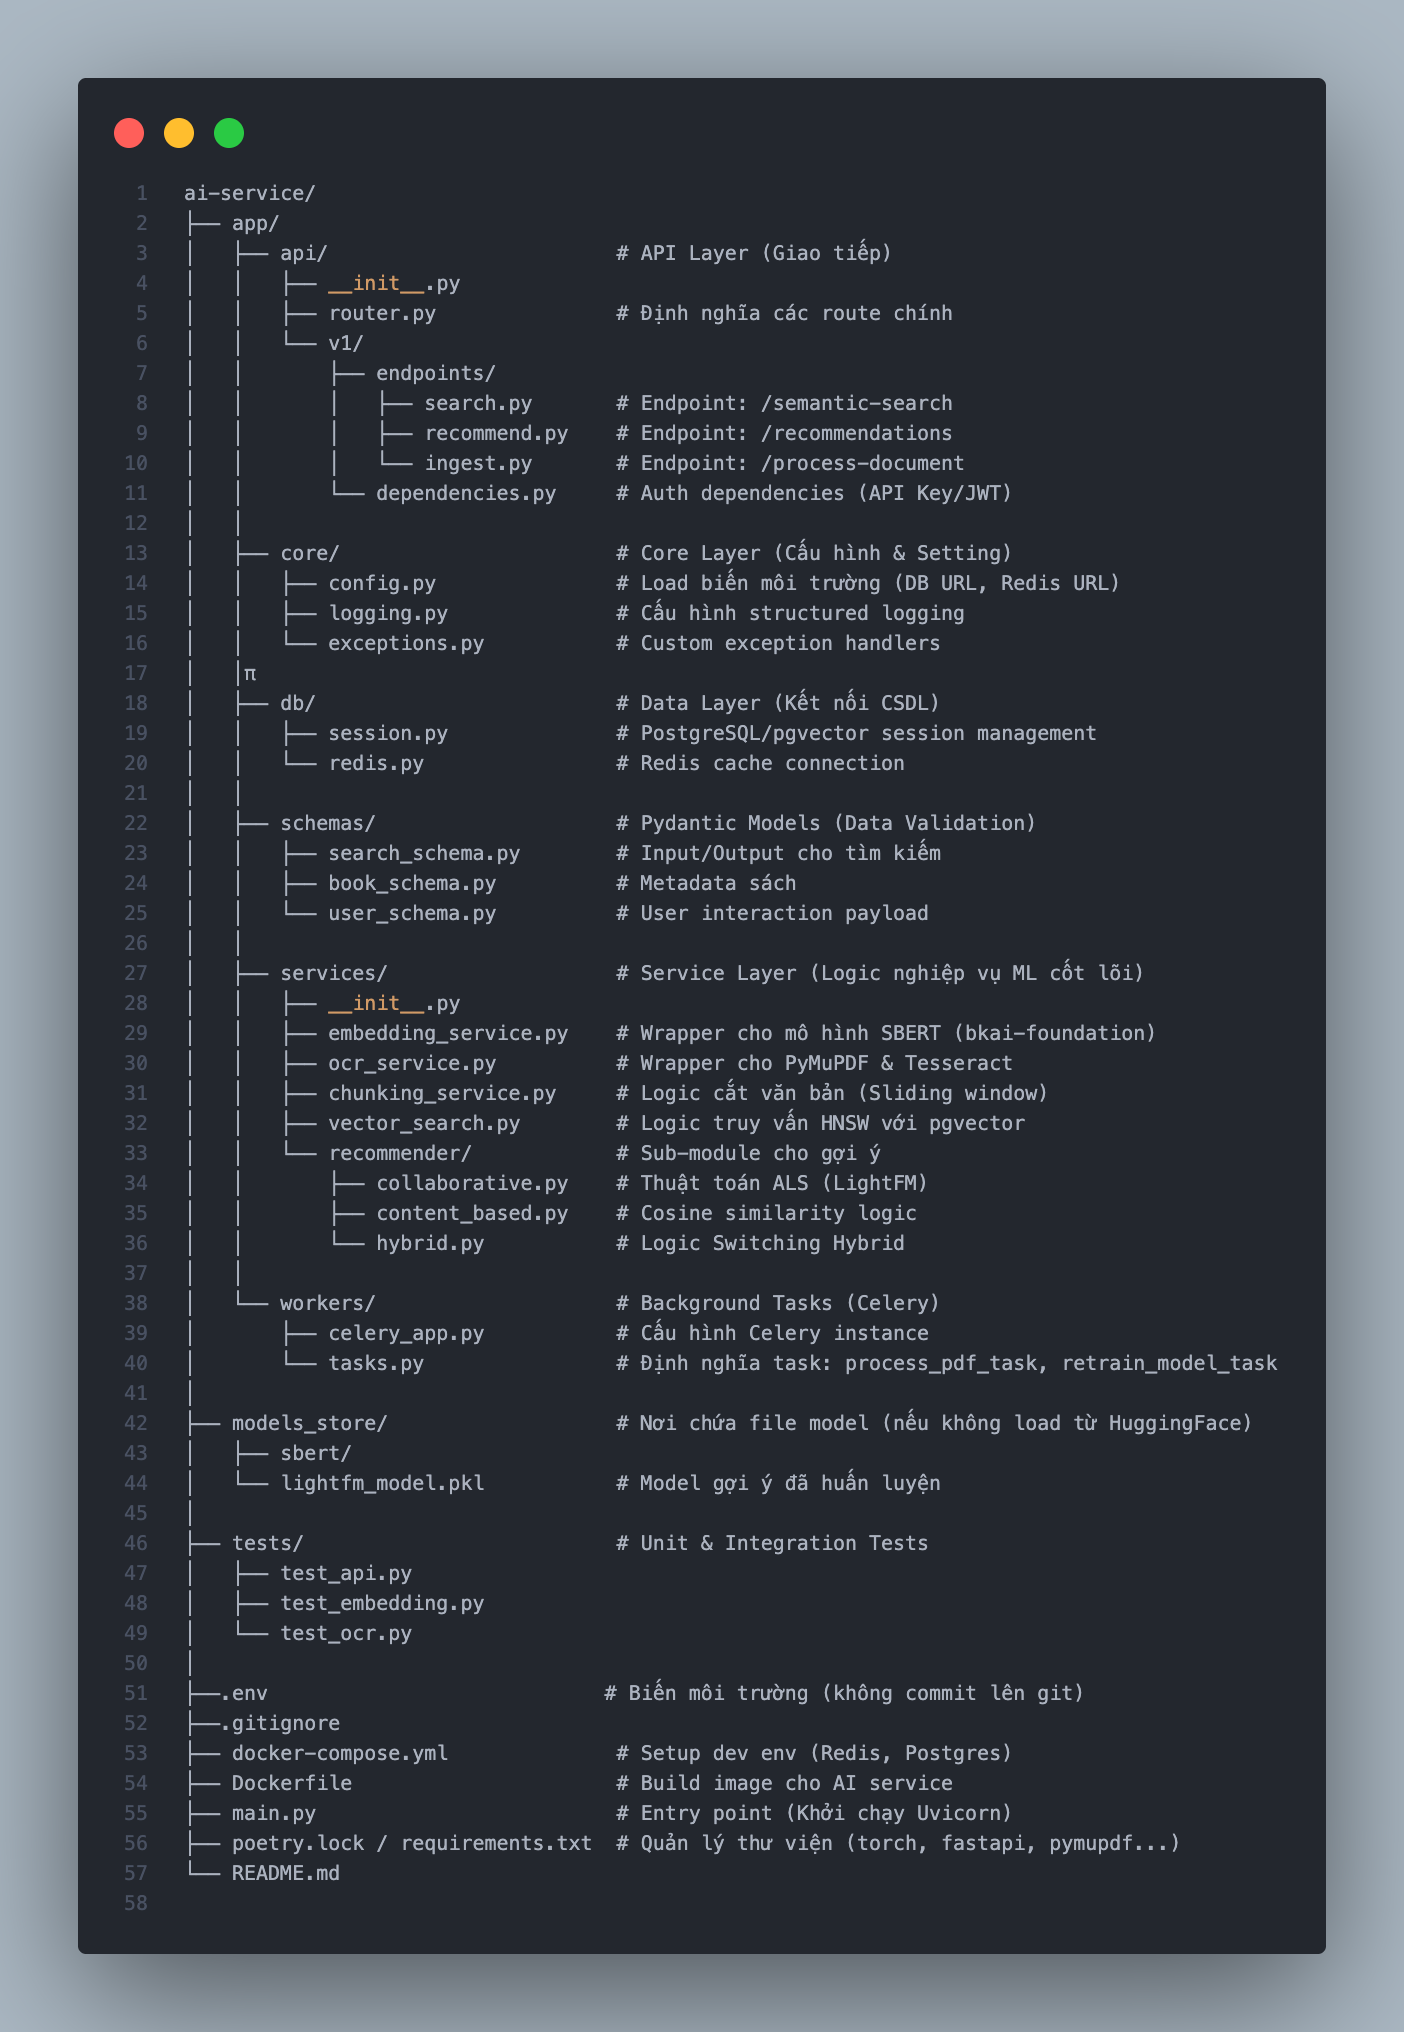
\includegraphics[width=0.95\linewidth]{images/V.Analysis_and_Design/architecture/ai_service_architecture.png}
\caption{Kiến trúc chi tiết AI Service và Luồng dữ liệu}
\label{fig:ai_service_architecture_detail}
\end{figure}


%-----------------------------AI-----------------------------------


\subsubsection{Luồng giao tiếp (Communication Flows) nâng cao}

Hệ thống sử dụng hai pattern giao tiếp chính: \textbf{Synchronous Communication} (REST API) cho các tương tác real-time cần phản hồi ngay lập tức, và \textbf{Asynchronous Communication} (Domain Events + Message Queue) cho các tác vụ có thể xử lý sau hoặc cần loose coupling giữa các modules.

\textbf{1. Giao tiếp đồng bộ (Synchronous Communication - REST API):}

Được sử dụng khi:
\begin{itemize}
    \item Frontend cần phản hồi ngay lập tức để hiển thị cho người dùng.
    \item Thao tác đọc dữ liệu (queries) không có side effects.
    \item Validation errors cần trả về trực tiếp cho người dùng.
    \item Cần đảm bảo transaction hoàn thành trước khi tiếp tục workflow.
\end{itemize}

\textbf{Ví dụ 1: Semantic Search Flow}
Luồng tìm kiếm ngữ nghĩa yêu cầu phản hồi nhanh để UX tốt:

\begin{enumerate}
    \item User nhập query "sách về machine learning" trên giao diện tìm kiếm.
    
    \item \texttt{Next.js Frontend} gửi \texttt{POST /api/v1/search/semantic} đến Backend Monolith với payload JSON chứa query string, limit, và filters.).
    
   \item \texttt{Backend} (Search Gateway Service) xử lý:
    \begin{itemize}
        \item Validate JWT token và extract user info.
        \item Check cache trong Redis với key: hash(query + filters).
        \item Nếu cache hit → return cached results ngay (< 50ms).
        \item Nếu cache miss → forward request đến AI Service qua internal network.
    \end{itemize}
    
    \item \texttt{Backend} gọi \texttt{POST http://ai-service:8000/api/ai/semantic-search} 
    (internal URL, không expose ra internet).
    
    \item \texttt{AI Service} xử lý:
    \begin{itemize}
        \item Embedding Service chuyển query thành vector 768 chiều.
        \item Vector Search Service thực hiện ANN search trong Vector DB.
        \item Trả về danh sách book IDs với similarity scores.
    \end{itemize}
    
    \item \texttt{Backend} nhận response từ AI Service:
    \begin{itemize}
        \item Cache kết quả trong Redis với Time-To-Live 1 hour.
        \item Log request (userId, query, resultCount, responseTime) để phân tích.
    \end{itemize}
    
    \item \texttt{Backend} query PostgreSQL để lấy metadata chi tiết 
    (title, author, cover, availability) của các book IDs.
    
    \item \texttt{Backend} merge AI results + metadata, trả về Frontend.
    
    \item Frontend render kết quả tìm kiếm.
\end{enumerate}

\textbf{Đặc điểm kỹ thuật:}
\begin{itemize}
    \item \textbf{Request-Response pattern:} Client chờ response trước khi tiếp tục (blocking call).
    \item \textbf{Timeout handling:} Frontend set timeout 5 giây, hiển thị error message nếu service không phản hồi.
    \item \textbf{Retry logic:} Tự động retry 2 lần với exponential backoff (1s, 2s) nếu gặp lỗi network transient.
    \item \textbf{Circuit breaker:} Sau 5 requests liên tiếp fail, tạm ngừng gọi AI Service 30 giây, fallback sang keyword search.
\end{itemize}

\textbf{2. Giao tiếp bất đồng bộ - Sự kiện nội bộ (Asynchronous Communication - Internal Events) (In-Memory Event Bus):}

Sử dụng Spring ApplicationEventPublisher cho giao tiếp giữa các modules trong Backend Monolith.

\textbf{Đặc điểm:}
\begin{itemize}
    \item Sự kiện được phát (publish) ngay sau khi giao dịch (transaction) hoàn tất thành công (sử dụng \texttt{@TransactionalEventListener}).
    \item Nhiều bộ lắng nghe (listeners) có thể cùng đăng ký (subscribe) một sự kiện (mô hình publish-subscribe).
    \item Các bộ lắng nghe được thực thi trong các giao dịch riêng biệt (separate transactions) để tránh ảnh hưởng lẫn nhau.
\end{itemize}
\textbf{Ví dụ 3: Quy trình Trả sách và Tính toán Phạt (Return Book with Fine Calculation)}

Khi người dùng trả sách, hàng loạt các tác vụ phụ (side effects) cần được thực hiện. Tuy nhiên, để đảm bảo trải nghiệm người dùng, các tác vụ này không được phép làm chặn (block) phản hồi của API chính:

\begin{enumerate}
    \item Người dùng thực hiện trả sách thông qua API \texttt{POST /api/v1/lending/return}.
    
    \item \texttt{ReturnBookUseCase} bên trong \textbf{Mô-đun Mượn trả (Lending Module)} thực hiện:
    \begin{itemize}
        \item Tải \texttt{BorrowTransaction} (Giao dịch mượn) từ cơ sở dữ liệu.
        \item Cập nhật trạng thái giao dịch: \texttt{BORROWING} $\rightarrow$ \texttt{RETURNED}.
        \item Kiểm tra hư hại (Check damage) $\rightarrow$ Xác nhận không hư hại.
        \item Tính toán trễ hạn (nếu \texttt{returnDate} > \texttt{dueDate}).
        \item Lưu giao dịch vào cơ sở dữ liệu.
        \item Phát sự kiện (Publish) \texttt{BookReturnedEvent} chứa thông tin: \texttt{transactionId}, \texttt{userId}, \texttt{itemId}, \texttt{returnDate}, \texttt{isOverdue}, \texttt{daysOverdue}.
    \end{itemize}
    
    \item Giao dịch cơ sở dữ liệu hoàn tất (Transaction commit) $\rightarrow$ Sự kiện được điều phối (dispatch) đến các bộ lắng nghe (listeners).
    
    \item \textbf{Mô-đun Phạt (Fine Module)} lắng nghe sự kiện \texttt{BookReturnedEvent}:
    \begin{itemize}
        \item Kiểm tra điều kiện: \texttt{event.isOverdue() == true}.
        \item Gọi \texttt{CalculateFineUseCase} với số ngày quá hạn.
        \item Tạo đối tượng tổng hợp \texttt{Fine} (Aggregate) với số tiền = \texttt{daysOverdue} $\times$ \texttt{dailyFineRate}.
        \item Lưu thông tin phạt vào cơ sở dữ liệu.
        \item Phát sự kiện \texttt{FineIncurredEvent} (Sự kiện phát sinh phí phạt).
    \end{itemize}
    
    \item \textbf{Mô-đun Người dùng (User Module)} lắng nghe sự kiện \texttt{BookReturnedEvent}:
    \begin{itemize}
        \item Nếu quá hạn (overdue): Giảm điểm tín nhiệm (credit score) -5 điểm.
        \item Nếu đúng hạn (on-time): Tăng điểm tín nhiệm +1 điểm.
        \item Cập nhật \texttt{user.creditScore} trong cơ sở dữ liệu.
    \end{itemize}
    
    \item \textbf{Mô-đun Người dùng} cũng lắng nghe sự kiện \texttt{FineIncurredEvent}:
    \begin{itemize}
        \item Cộng dồn số tiền phạt vào \texttt{user.totalOutstandingFines} (Tổng nợ phạt hiện tại).
        \item Nếu \texttt{totalOutstandingFines} > 500,000 VNĐ $\rightarrow$ Cấm người dùng (chuyển trạng thái = \texttt{BANNED}).
    \end{itemize}
    
    \item \textbf{Mô-đun Danh mục (Catalog Module)} lắng nghe sự kiện \texttt{BookReturnedEvent}:
    \begin{itemize}
        \item Cập nhật trạng thái bản sao (Item status): \texttt{BORROWED} $\rightarrow$ \texttt{AVAILABLE}.
        \item Tăng biến đếm số lượng khả dụng (\texttt{availableCount}).
        \item Phát sự kiện \texttt{ItemReturnedEvent}.
    \end{itemize}
    
    \item \textbf{Mô-đun Mượn trả (Lending Module)} lắng nghe sự kiện \texttt{ItemReturnedEvent}:
    \begin{itemize}
        \item Kích hoạt \texttt{ProcessReservationQueueUseCase} (Xử lý hàng đợi đặt chỗ).
        \item Tìm người dùng ưu tiên đầu tiên trong hàng đợi đặt chỗ cho ấn phẩm này.
        \item Gửi thông báo: "Sách bạn đặt đã có sẵn, vui lòng đến lấy trong vòng 24 giờ".
        \item Thiết lập thời gian hết hạn giữ sách (\texttt{hold expiration}) = thời điểm hiện tại + 24 giờ.
    \end{itemize}
\end{enumerate}

\textbf{Lợi ích của Internal Events:}
\begin{itemize}
    \item \textbf{Decoupling:} Lending Module không biết Fine Module, User Module, Catalog Module tồn tại. Chỉ cần publish event, không quan tâm ai consume.
    \item \textbf{Single Responsibility:} Mỗi module chỉ quan tâm đến domain logic của mình.
    \item \textbf{Extensibility:} Thêm listener mới (ví dụ: Notification Module gửi email) không cần sửa code Lending Module.
    \item \textbf{Transaction safety:} Events chỉ publish sau khi transaction commit thành công. Nếu transaction rollback, events không được trigger.
    \item \textbf{Testability:} Có thể test từng listener độc lập bằng cách publish fake events.
\end{itemize}

\textbf{3. Giao tiếp Bất đồng bộ - Sự kiện Bên ngoài (Hàng đợi Thông điệp):}

Sử dụng \textbf{RabbitMQ} cho giao tiếp giữa Backend Monolith và Dịch vụ AI (giao tiếp liên tiến trình - cross-process communication).

\textbf{Đặc điểm kỹ thuật:}
\begin{itemize}
    \item \textbf{Thông điệp bền vững (Persistent Messages):} Dữ liệu không bị mất ngay cả khi máy chủ khởi động lại.
    \item \textbf{Đảm bảo giao nhận (Guaranteed Delivery):} Tích hợp cơ chế thử lại (retry mechanism) khi có lỗi.
    \item \textbf{Hàng đợi Thư chết (Dead Letter Queue - DLQ):} Nơi lưu trữ các thông điệp thất bại sau nhiều lần thử lại để xử lý sau.
    \item \textbf{Xác nhận từ người tiêu thụ (Consumer Acknowledgment):} Đảm bảo thông điệp chỉ được xóa khỏi hàng đợi khi đã xử lý thành công.
\end{itemize}

\textbf{Ví dụ 4: Quy trình Thêm sách mới kèm Xử lý PDF (Add Book with PDF Processing)}

Quá trình xử lý PDF tốn nhiều thời gian (OCR 100 trang có thể mất 5-10 phút), do đó không thể sử dụng cơ chế chặn (blocking) API:

\begin{enumerate}
    \item Thủ thư tải lên sách mới thông qua API \texttt{POST /api/v1/books} với định dạng form-data chứa tệp PDF và siêu dữ liệu (tiêu đề, tác giả, ISBN).
    
    \item \texttt{AddBookUseCase} trong \textbf{Mô-đun Danh mục (Catalog Module)} thực hiện:
    \begin{itemize}
        \item Kiểm tra hợp lệ siêu dữ liệu (định dạng ISBN, các trường bắt buộc).
        \item Tải tệp PDF lên MinIO/S3, nhận về \texttt{pdfUrl}.
        \item Tạo đối tượng tổng hợp \texttt{Publication} với trạng thái \texttt{processingStatus = PENDING}.
        \item Tạo \texttt{Item} cho mỗi bản sao vật lý.
        \item Lưu dữ liệu vào PostgreSQL.
        \item Phát sự kiện \texttt{BookAddedEvent} lên RabbitMQ exchange \texttt{book.events} với khóa định tuyến (routing key) \texttt{book.added}.
    \end{itemize}
    
    \item API trả về mã HTTP 201 Created ngay lập tức (< 500ms) kèm phản hồi: \texttt{publicationId}, \texttt{processingStatus: PENDING}, \texttt{estimatedCompletionTime}: "5-10 minutes".
    
    \item Thủ thư nhận thông báo "Sách đã được thêm. Đang xử lý nội dung PDF..." và có thể tiếp tục thực hiện công việc khác mà không phải chờ đợi.
    
    \item \textbf{Dịch vụ AI} có các Celery worker tiêu thụ thông điệp từ hàng đợi \texttt{book.processing.queue}:
    \begin{itemize}
        \item Worker nhận thông điệp chứa: \texttt{publicationId}, \texttt{pdfUrl}, \texttt{metadata}.
        \item Tải PDF từ MinIO (dạng luồng - streaming để tiết kiệm bộ nhớ).
        \item Dịch vụ OCR trích xuất văn bản từng trang (sử dụng Tesseract/PaddleOCR).
        \item Dịch vụ Phân mảnh văn bản (Text Chunking) chia văn bản thành các đoạn 512 tokens, độ chồng lấn (overlap) 50 tokens.
        \item Dịch vụ Vector hóa (Embedding Service) tạo vector cho mỗi đoạn (xử lý theo lô - batch processing 10 chunks/lần).
        \item Lưu vào CSDL Vector: bảng \texttt{publication\_vectors} với các cột (\texttt{publication\_id}, \texttt{chunk\_id}, \texttt{embedding}, \texttt{chunk\_text}, \texttt{page\_num}).
        \item Nếu bất kỳ bước nào thất bại $\rightarrow$ ném ra ngoại lệ (throw exception), thông điệp tự động được thử lại (tối đa 3 lần).
    \end{itemize}
    
    \item Sau khi hoàn tất (hoặc thất bại sau tất cả lần thử):
    \begin{itemize}
        \item Worker gọi REST API phản hồi (callback) về Backend: \texttt{POST /api/v1/books/\{id\}/processing-complete} với trạng thái: \texttt{SUCCESS} hoặc \texttt{FAILED}.
        \item Backend cập nhật \texttt{processingStatus} trong cơ sở dữ liệu.
        \item Gửi thông báo cho thủ thư: "PDF đã xử lý xong" hoặc "Xử lý PDF thất bại".
    \end{itemize}
    
    \item Kết quả: Nếu xử lý thành công, sách xuất hiện trong kết quả tìm kiếm ngữ nghĩa. Nếu thất bại, sách vẫn có trong danh mục nhưng chỉ hỗ trợ tìm kiếm theo từ khóa truyền thống.
\end{enumerate}

\textbf{Đặc điểm của Mẫu thiết kế Hàng đợi Thông điệp (Message Queue Pattern):}
\begin{itemize}
    \item \textbf{Xử lý bất đồng bộ (Async processing):} Backend không bị chặn (non-blocking), trả phản hồi ngay lập tức cho người dùng để tối ưu trải nghiệm.
    \item \textbf{Cơ chế thử lại (Retry mechanism):} RabbitMQ tự động thử lại nếu Dịch vụ AI gặp lỗi tạm thời (hết thời gian chờ mạng, dịch vụ bận).
    \item \textbf{Hàng đợi Thư chết (DLQ):} Các thông điệp bị lỗi sau 3 lần thử lại được chuyển sang DLQ để quản trị viên điều tra và xử lý thủ công (ví dụ: tệp PDF bị hỏng).
    \item \textbf{Giao nhận ít nhất một lần (At-least-once delivery):} Thông điệp có thể được giao nhiều lần (do mạng thử lại). Dịch vụ AI phải đảm bảo tính lũy đẳng (idempotent): kiểm tra xem \texttt{publicationId} đã được xử lý chưa trước khi thực hiện.
    \item \textbf{Cân bằng tải (Load balancing):} Nếu có nhiều instance của Dịch vụ AI, RabbitMQ tự động phân phối thông điệp (theo thuật toán round-robin).
    \item \textbf{Áp lực ngược (Backpressure):} Nếu Dịch vụ AI quá tải, thông điệp sẽ xếp hàng trong queue, Backend vẫn nhận yêu cầu bình thường mà không bị sập.
\end{itemize}

\textbf{4. Chuỗi sự kiện lan truyền - Quy trình nghiệp vụ đa mô-đun phức tạp (Event Cascade)}

Một số quy trình công việc (workflows) đòi hỏi sự kết hợp giữa cả gọi đồng bộ (sync calls) và sự kiện bất đồng bộ (async events) để đạt được sự cân bằng tối ưu giữa tính nhất quán dữ liệu (consistency) và hiệu năng (performance).

\textbf{Ví dụ 5: Quy trình Mượn sách hoàn chỉnh (Borrow Book - Complete Workflow)}

\begin{enumerate}
    \item \textbf{Giai đoạn 1: Kiểm tra hợp lệ Đồng bộ (Synchronous Validation)}
    \begin{itemize}
        \item Người dùng nhấn "Mượn sách" $\rightarrow$ Frontend gửi yêu cầu \texttt{POST /api/v1/lending/borrow}.
        \item \texttt{LendingController} kiểm tra tính hợp lệ của yêu cầu (Validation).
        \item \texttt{BorrowBookUseCase} gọi đồng bộ sang \textbf{Mô-đun Người dùng}: kiểm tra điểm tín nhiệm $\ge$ 50.
        \item \texttt{BorrowBookUseCase} gọi đồng bộ sang \textbf{Mô-đun Danh mục}: kiểm tra sách có sẵn (availability).
        \item Tạo \texttt{BorrowTransaction}, lưu vào cơ sở dữ liệu, và cam kết giao dịch (commit transaction).
        \item API trả về mã \texttt{201 Created} (tổng thời gian: $\sim$200ms).
    \end{itemize}
    
    \item \textbf{Giai đoạn 2: Sự kiện Nội bộ (In-Memory Internal Events)}
    \begin{itemize}
        \item \textbf{Mô-đun Mượn trả} phát sự kiện \texttt{BookBorrowedEvent}.
        \item \textbf{Mô-đun Người dùng} lắng nghe $\rightarrow$ tăng số lượng sách đang mượn (\texttt{currentBorrowCount}), cập nhật điểm tín nhiệm (nếu có chính sách).
        \item \textbf{Mô-đun Danh mục} lắng nghe $\rightarrow$ cập nhật trạng thái bản sao: \texttt{AVAILABLE} $\rightarrow$ \texttt{BORROWED}.
        \item \textbf{Mô-đun Tương tác (Engagement)} lắng nghe $\rightarrow$ ghi nhật ký hành vi người dùng (\texttt{userId}, \texttt{publicationId}, hành động: \texttt{BORROW}).
    \end{itemize}
    
    \item \textbf{Giai đoạn 3: Sự kiện Bên ngoài (External Events - RabbitMQ)}
    \begin{itemize}
        \item Backend phát sự kiện \texttt{BookBorrowedEvent} lên RabbitMQ.
        \item \textbf{Dịch vụ AI} tiêu thụ sự kiện $\rightarrow$ cập nhật vector sở thích người dùng (học tăng cường - incremental learning).
        \item Lên lịch huấn luyện lại mô hình gợi ý (retrain schedule) nếu tích lũy đủ 1000 tương tác mới.
    \end{itemize}
\end{enumerate}

\textbf{Dòng thời gian xử lý (Timeline):}
\begin{itemize}
    \item \textbf{T+0ms:} Người dùng nhấn nút "Mượn sách".
    \item \textbf{T+200ms:} API phản hồi \texttt{201 Created} $\rightarrow$ Người dùng thấy thông báo "Mượn sách thành công".
    \item \textbf{T+300ms:} Các sự kiện nội bộ hoàn tất $\rightarrow$ Cơ sở dữ liệu đạt trạng thái nhất quán (Consistent).
    \item \textbf{T+5s:} Dịch vụ AI cập nhật vector người dùng $\rightarrow$ Bộ máy gợi ý có dữ liệu mới nhất.
\end{itemize}

\textbf{Lợi ích kiến trúc:}
\begin{itemize}
    \item \textbf{Phản hồi nhanh (Fast response):} Người dùng không phải chờ AI xử lý xong mới mượn được sách.
    \item \textbf{Tính nhất quán mạnh (Strong consistency):} Giao dịch cốt lõi (bản ghi mượn sách, kho hàng) đảm bảo nhất quán tuyệt đối nhờ ACID transaction.
    \item \textbf{Tính nhất quán cuối cùng (Eventual consistency):} Dữ liệu gợi ý của AI đạt trạng thái nhất quán sau một khoảng thời gian ngắn (chấp nhận được trong nghiệp vụ).
    \item \textbf{Khả năng phục hồi (Resilience):} Nếu Dịch vụ AI gặp sự cố (down), chức năng mượn sách cốt lõi vẫn hoạt động bình thường, hệ thống chỉ tạm thời mất tính năng cập nhật gợi ý theo thời gian thực.
\end{itemize}

% =================================================================
% ======= NỘI DUNG CHO PHẦN THIẾT KẾ CƠ SỞ DỮ LIỆU =======
% =================================================================




\subsection{Thiết kế giao diện}

Toàn bộ giao diện hệ thống được thiết kế trên \textbf{Figma} trước khi hiện thực, đảm bảo sự thống nhất về phong cách (Design System) và luồng tương tác (User Flow) giữa các màn hình. Bản thiết kế đầy đủ có thể xem tại đường dẫn trong Phụ lục~\ref{appendix:resources}.

Hệ thống tuân thủ các nguyên tắc thiết kế cốt lõi: \textbf{tính nhất quán} (màu sắc, typography, hành vi component thống nhất toàn ứng dụng), \textbf{phản hồi trạng thái} (loading skeleton khi AI xử lý, toast notification sau thao tác), \textbf{tối giản} (nội dung trọng tâm là sách và thanh tìm kiếm), và \textbf{responsive} (Tailwind CSS Grid đảm bảo hiển thị tốt trên mọi thiết bị). Thư viện component \textbf{Shadcn/ui} được sử dụng để xây dựng các thành phần tái sử dụng nhất quán.

\subsubsection{Giao diện Public (Trang chủ và Tìm kiếm)}

\begin{figure}[htbp]
    \centering
    \begin{subfigure}[t]{0.48\linewidth}
        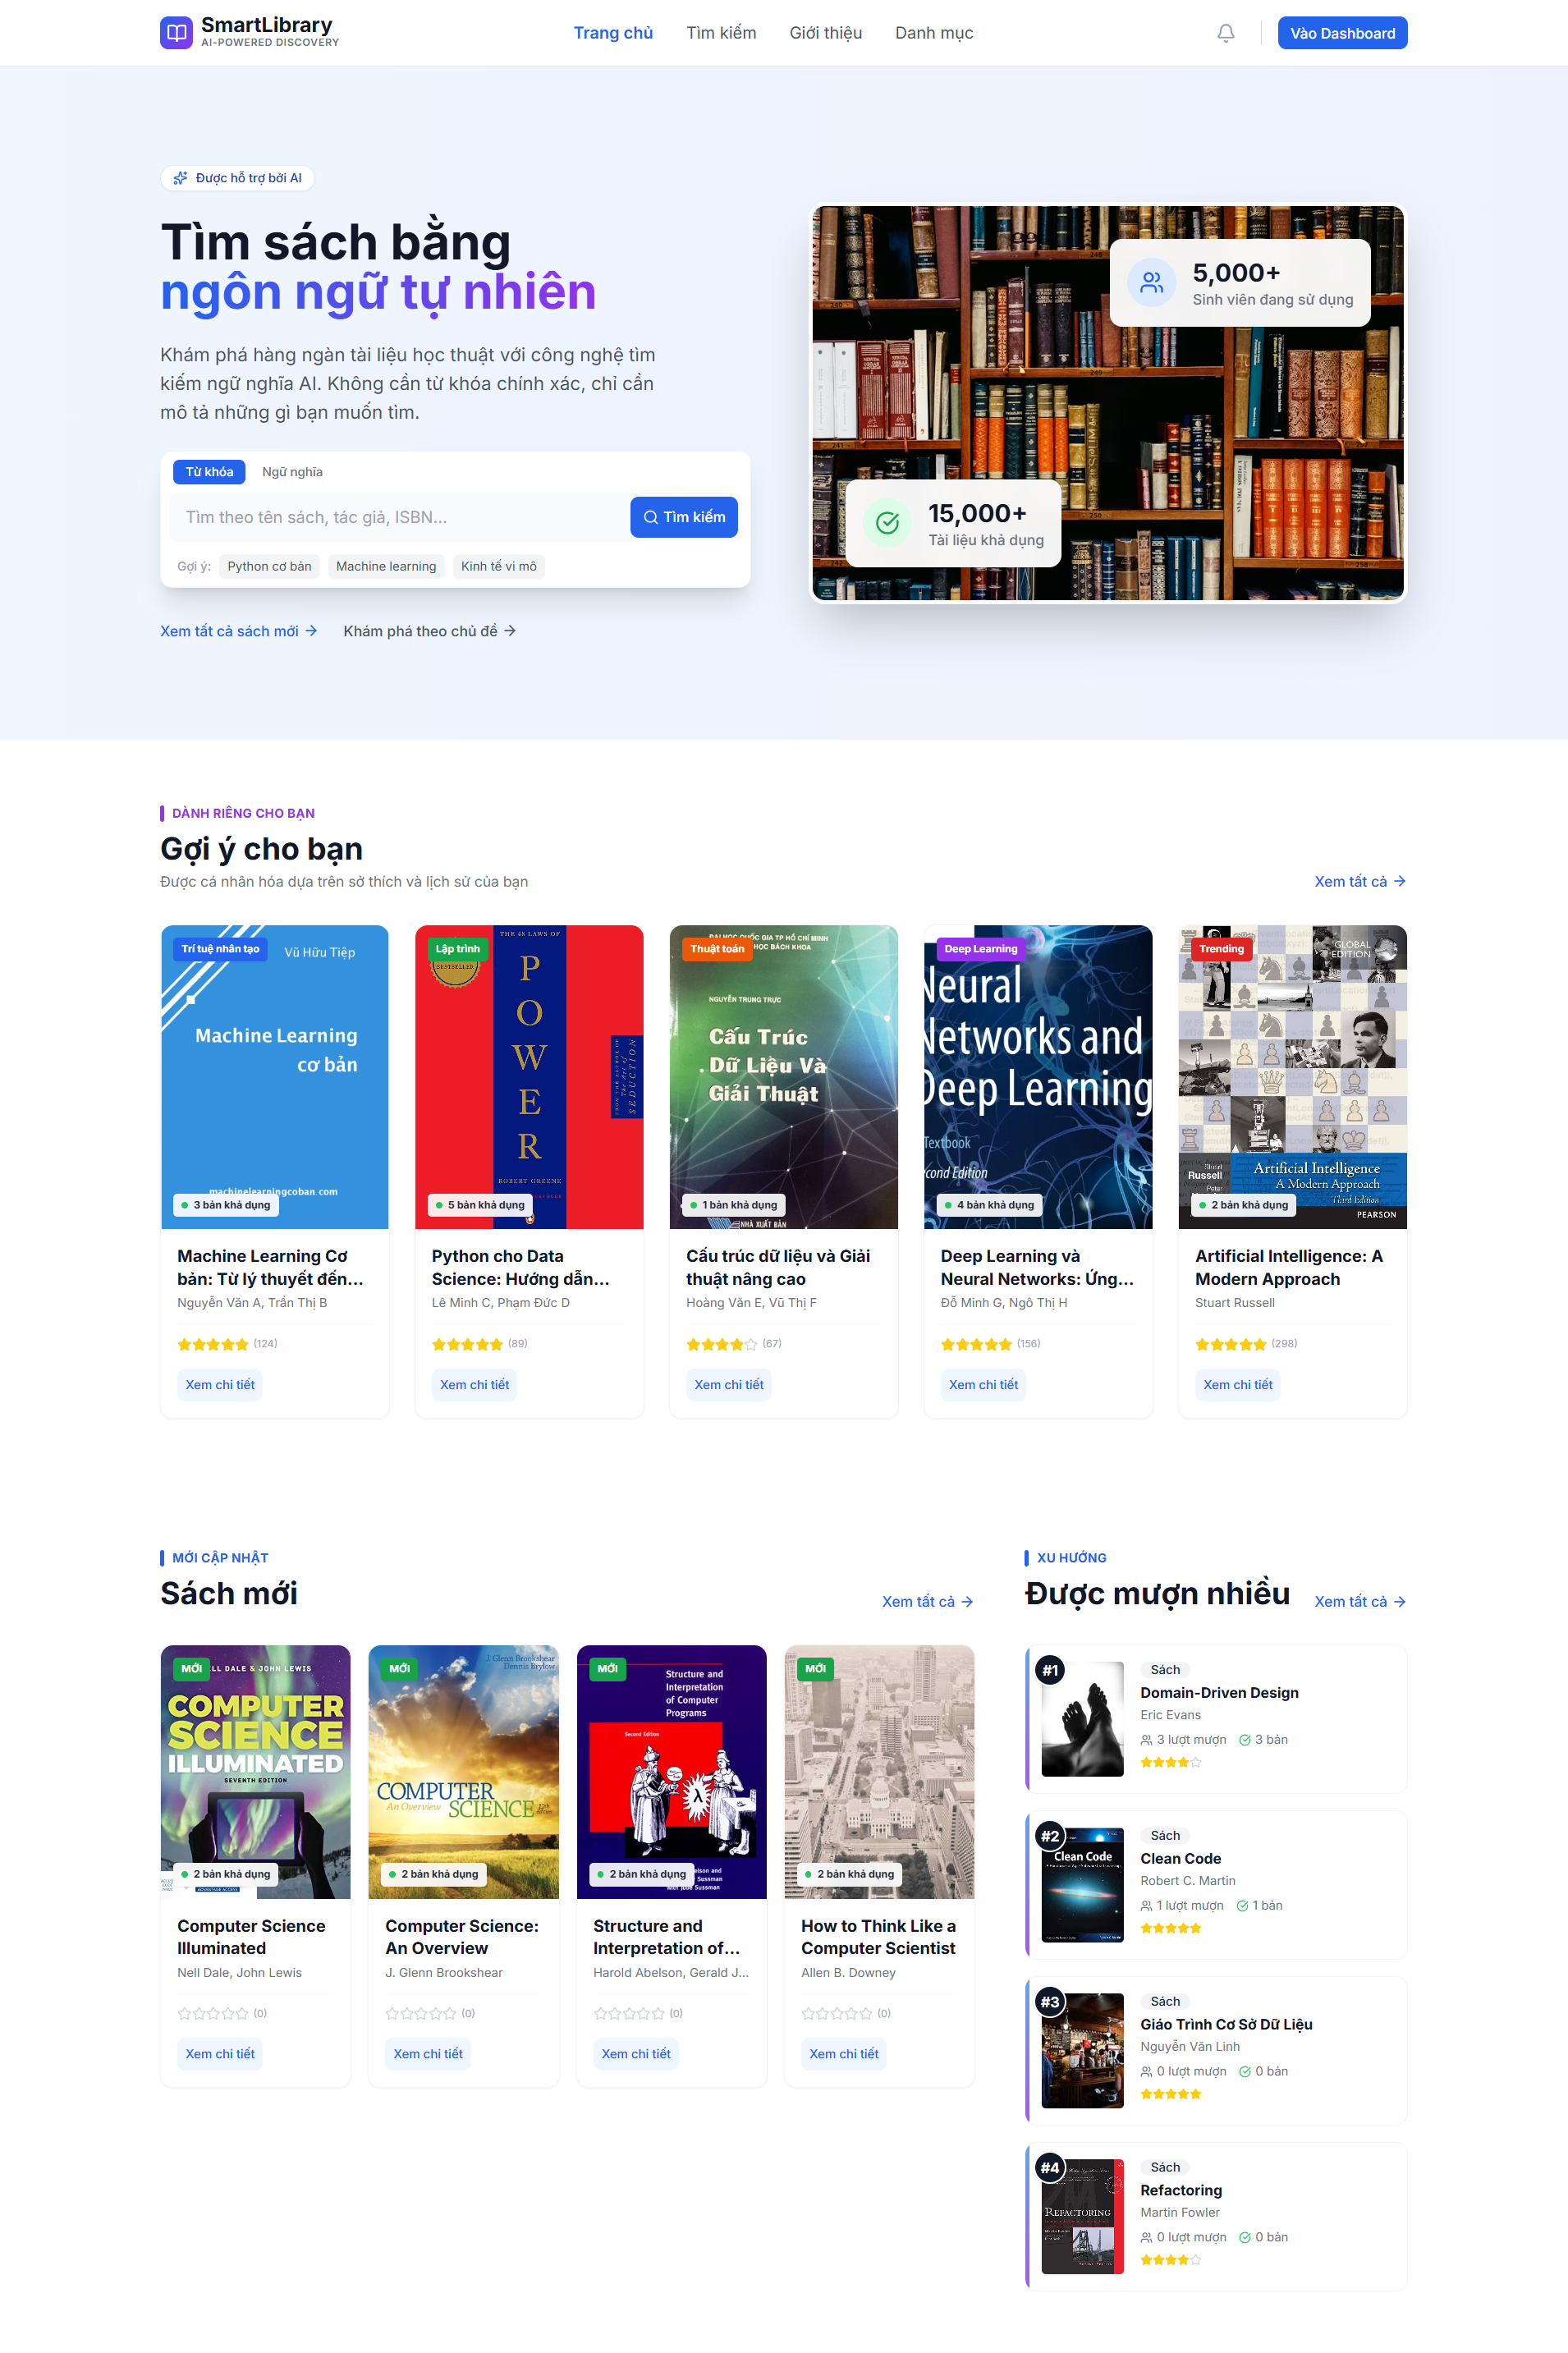
\includegraphics[width=\linewidth, height=0.38\textheight, keepaspectratio]{images/public_pages/Homepage_1.png}
        \caption{Trang chủ}
        \label{fig:home_page}
    \end{subfigure}
    \hfill
    \begin{subfigure}[t]{0.48\linewidth}
        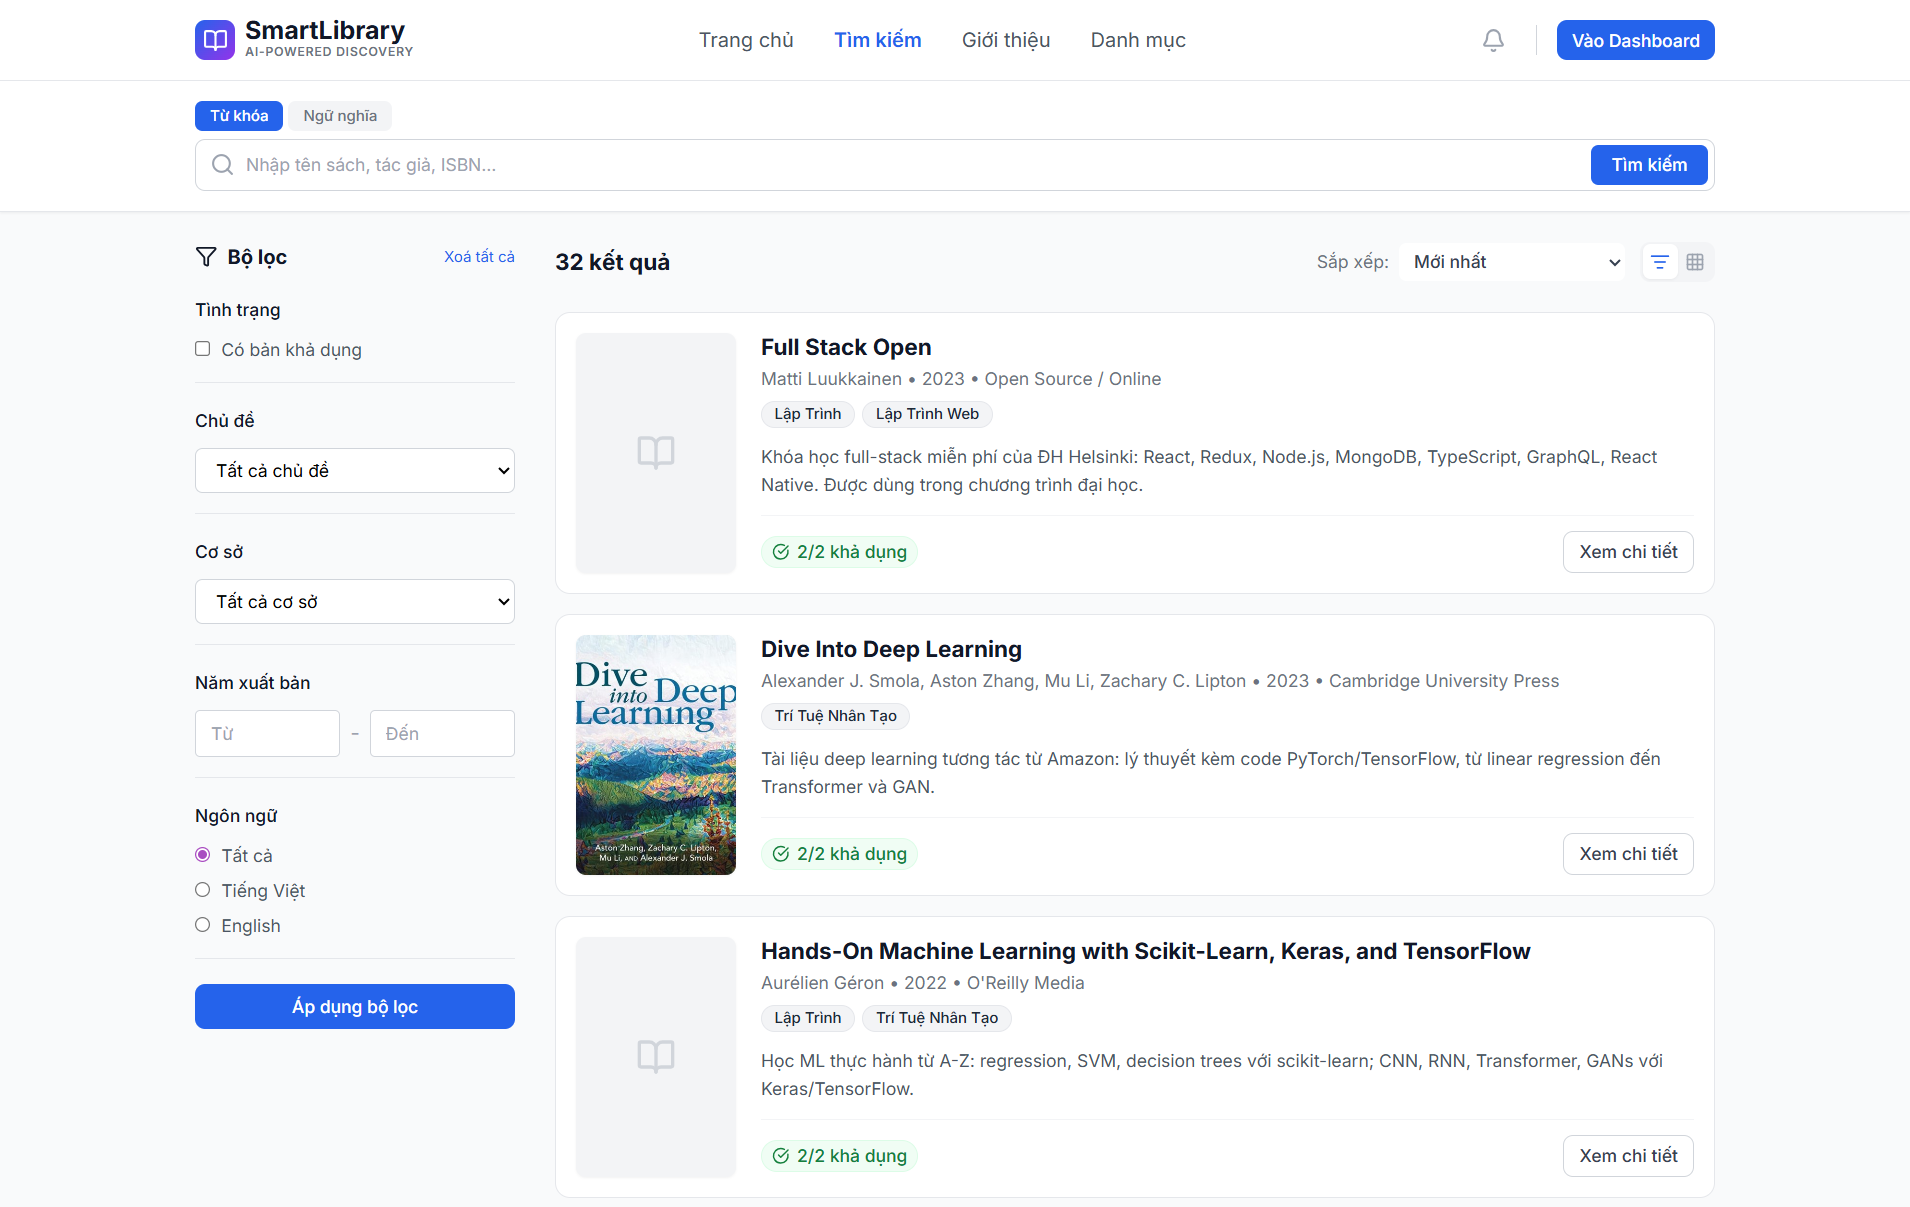
\includegraphics[width=\linewidth, height=0.38\textheight, keepaspectratio]{images/public_pages/Search_book.png}
        \caption{Tìm kiếm sách với bộ lọc}
        \label{fig:search_book}
    \end{subfigure}
    \caption{Giao diện Public: Trang chủ và Tìm kiếm}
\end{figure}


\begin{figure}[htbp]
    \centering
    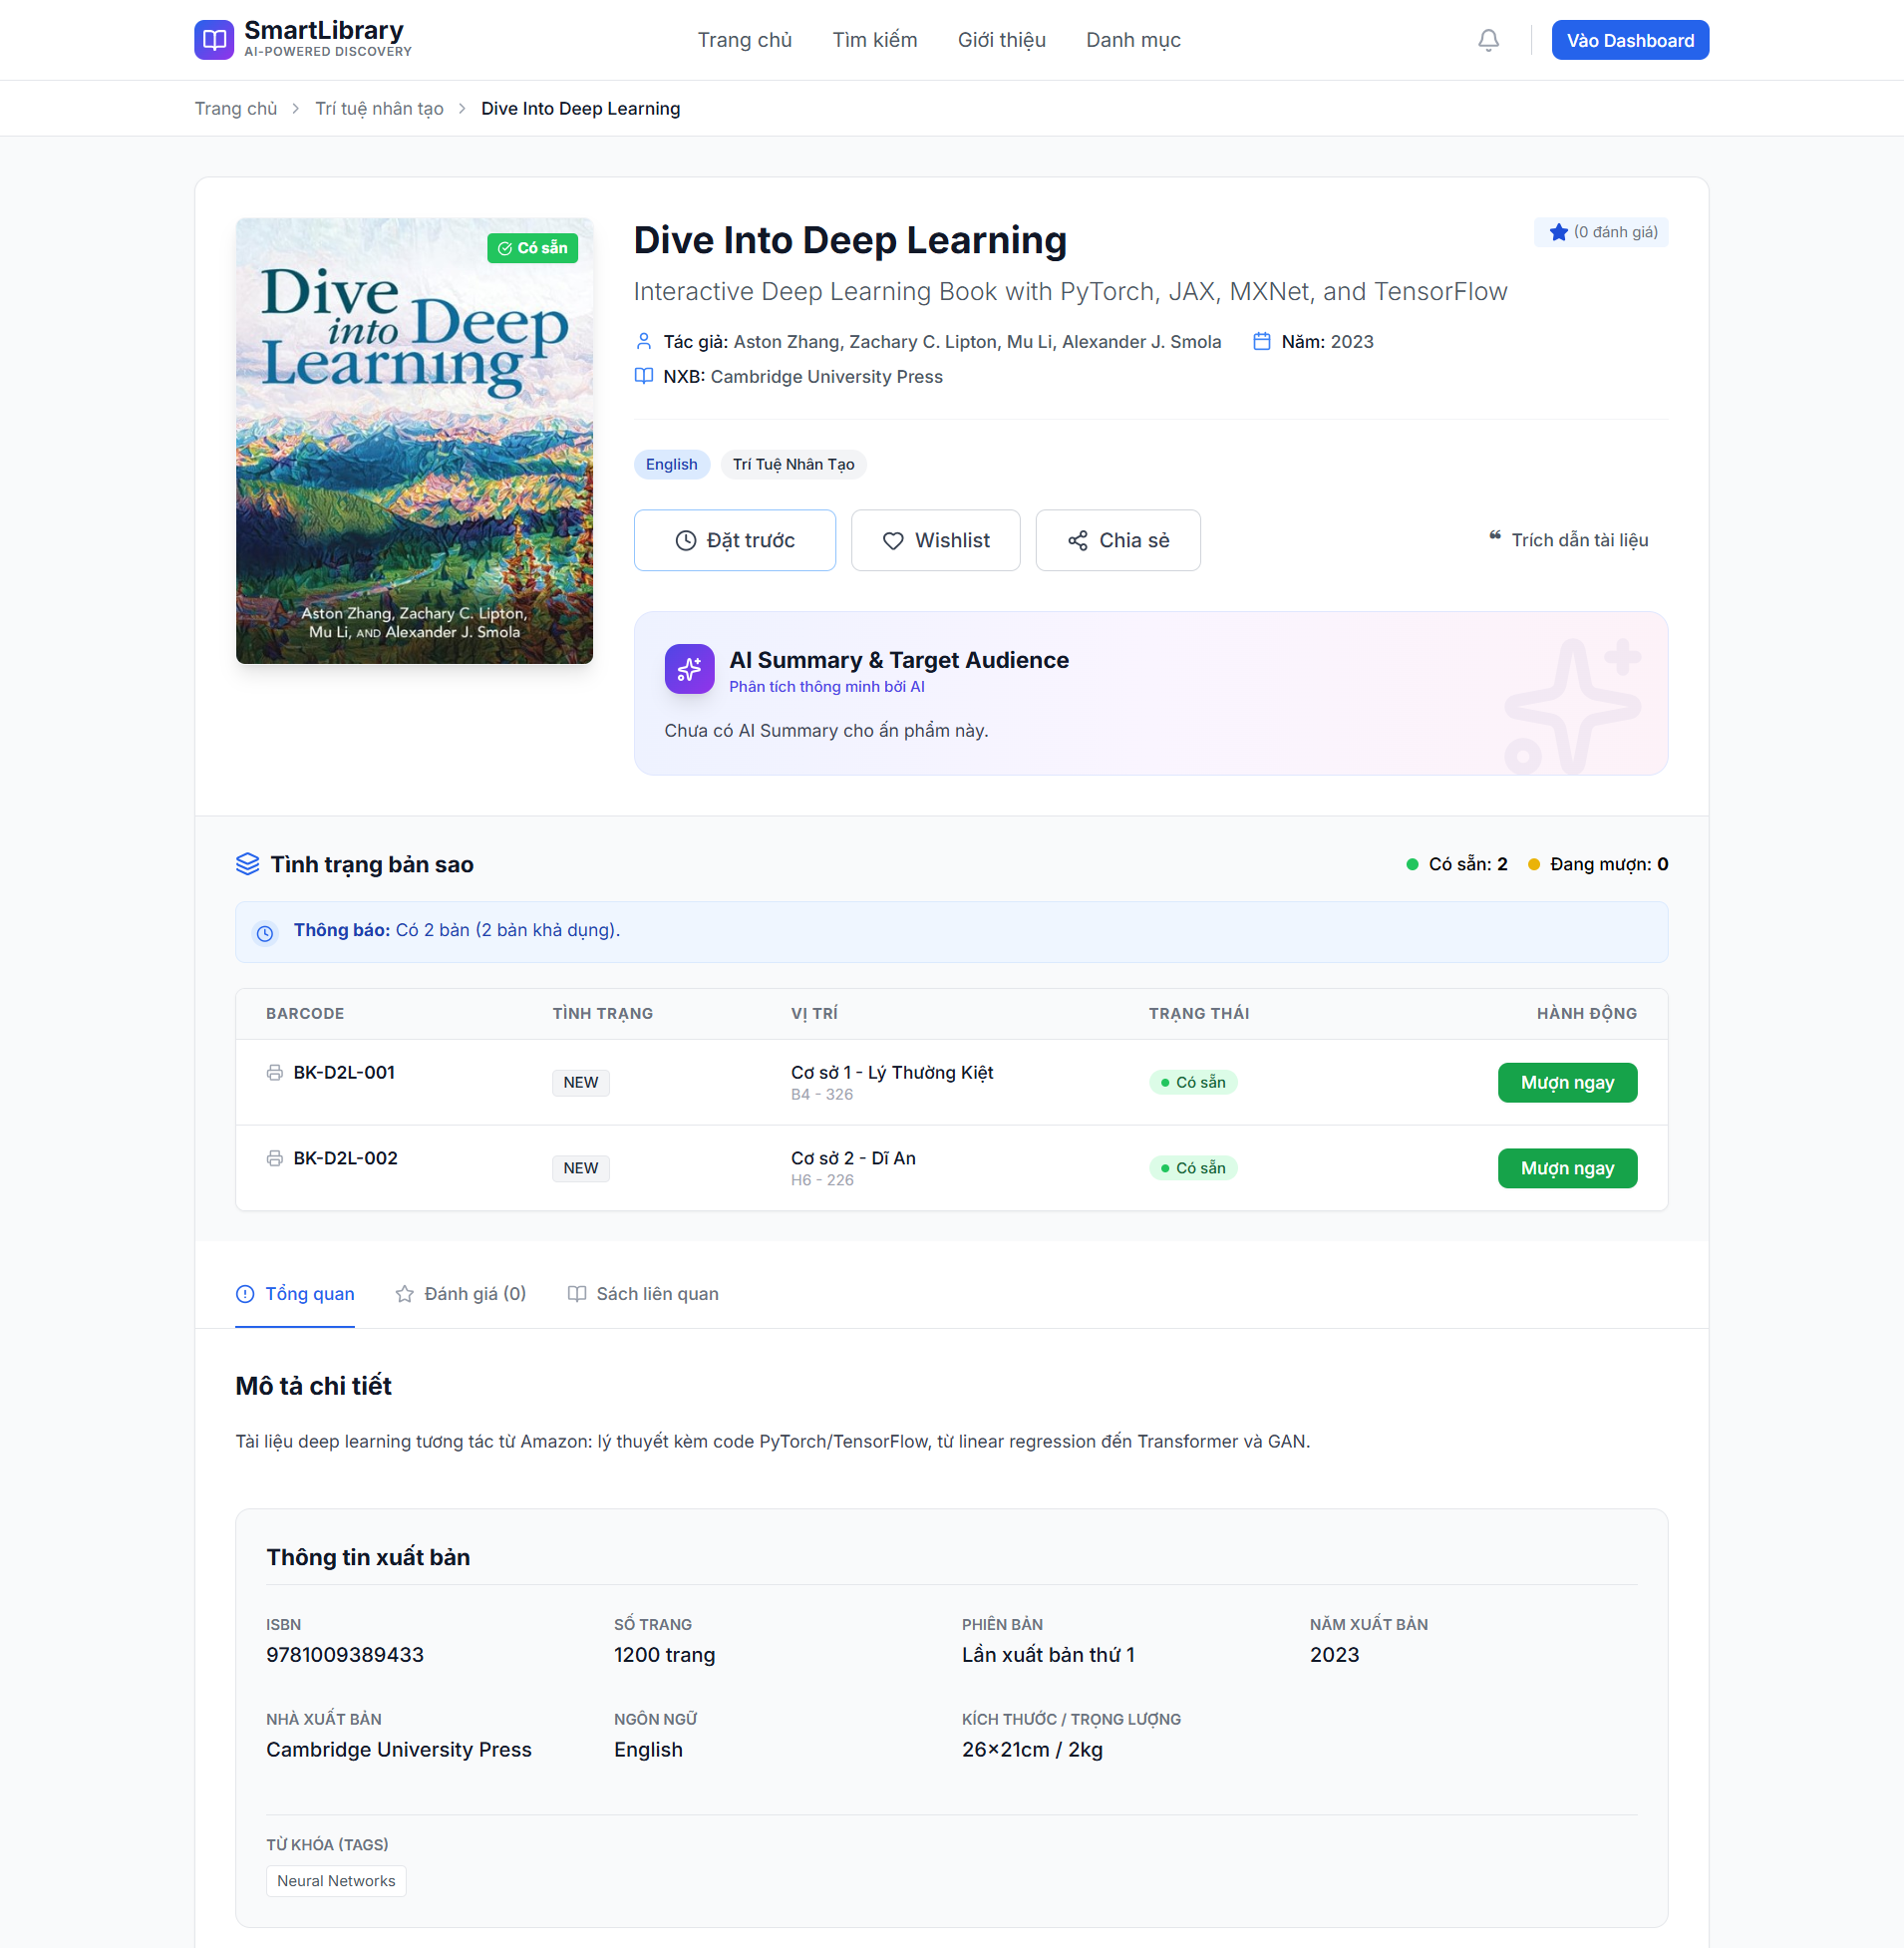
\includegraphics[width=0.6\linewidth]{images/public_pages/Book_detail.png}
    \caption{Giao diện Chi tiết sách}
    \label{fig:book_detail}
\end{figure}
\FloatBarrier

\subsubsection{Giao diện Độc giả (User Pages)}

\begin{figure}[htbp]
    \centering
    \begin{subfigure}[t]{0.48\linewidth}
        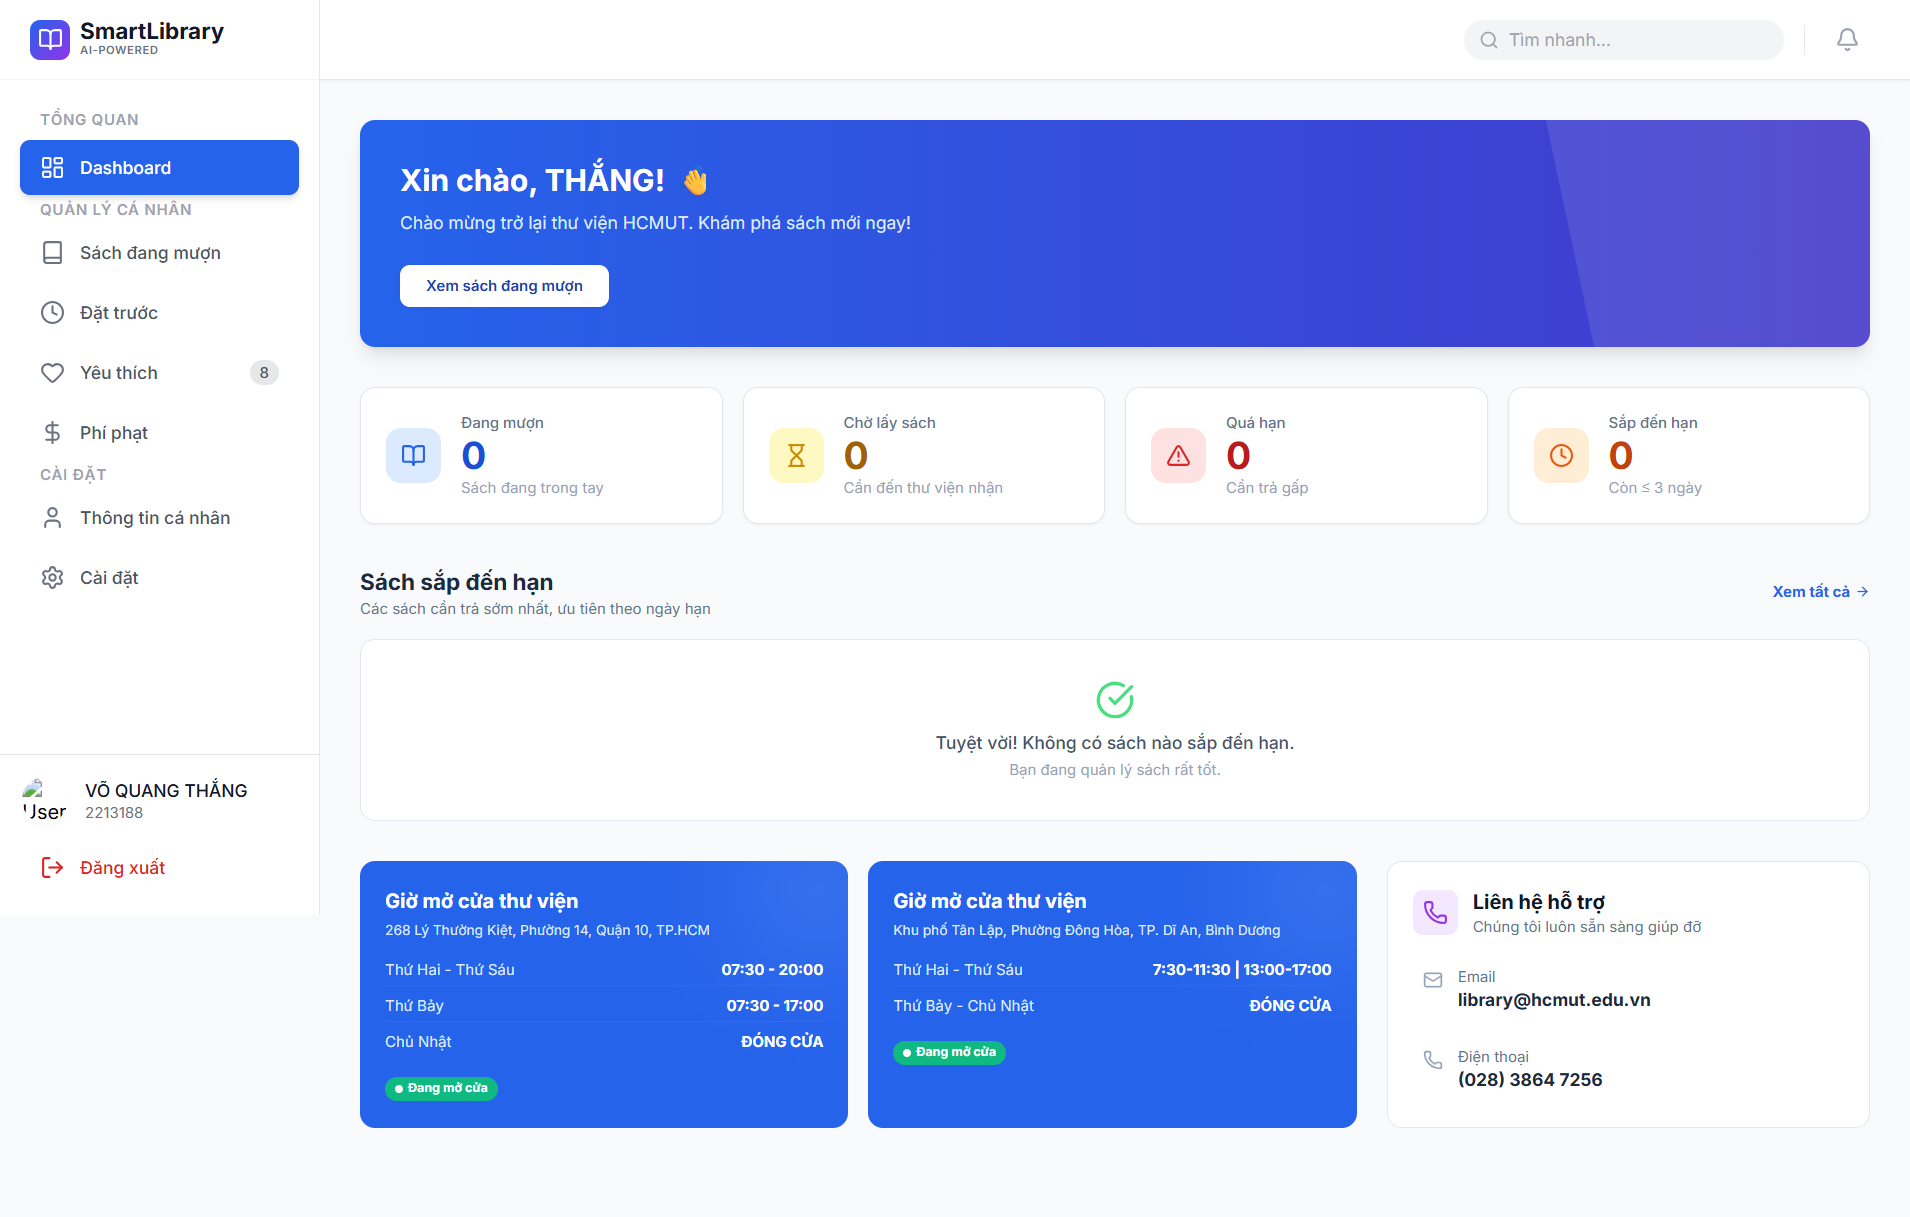
\includegraphics[width=\linewidth, height=0.38\textheight, keepaspectratio]{images/user_pages/Dashboard_reader_version_2.png}
        \caption{Dashboard tổng quan}
        \label{fig:user_dashboard}
    \end{subfigure}
    \hfill
    \begin{subfigure}[t]{0.48\linewidth}
        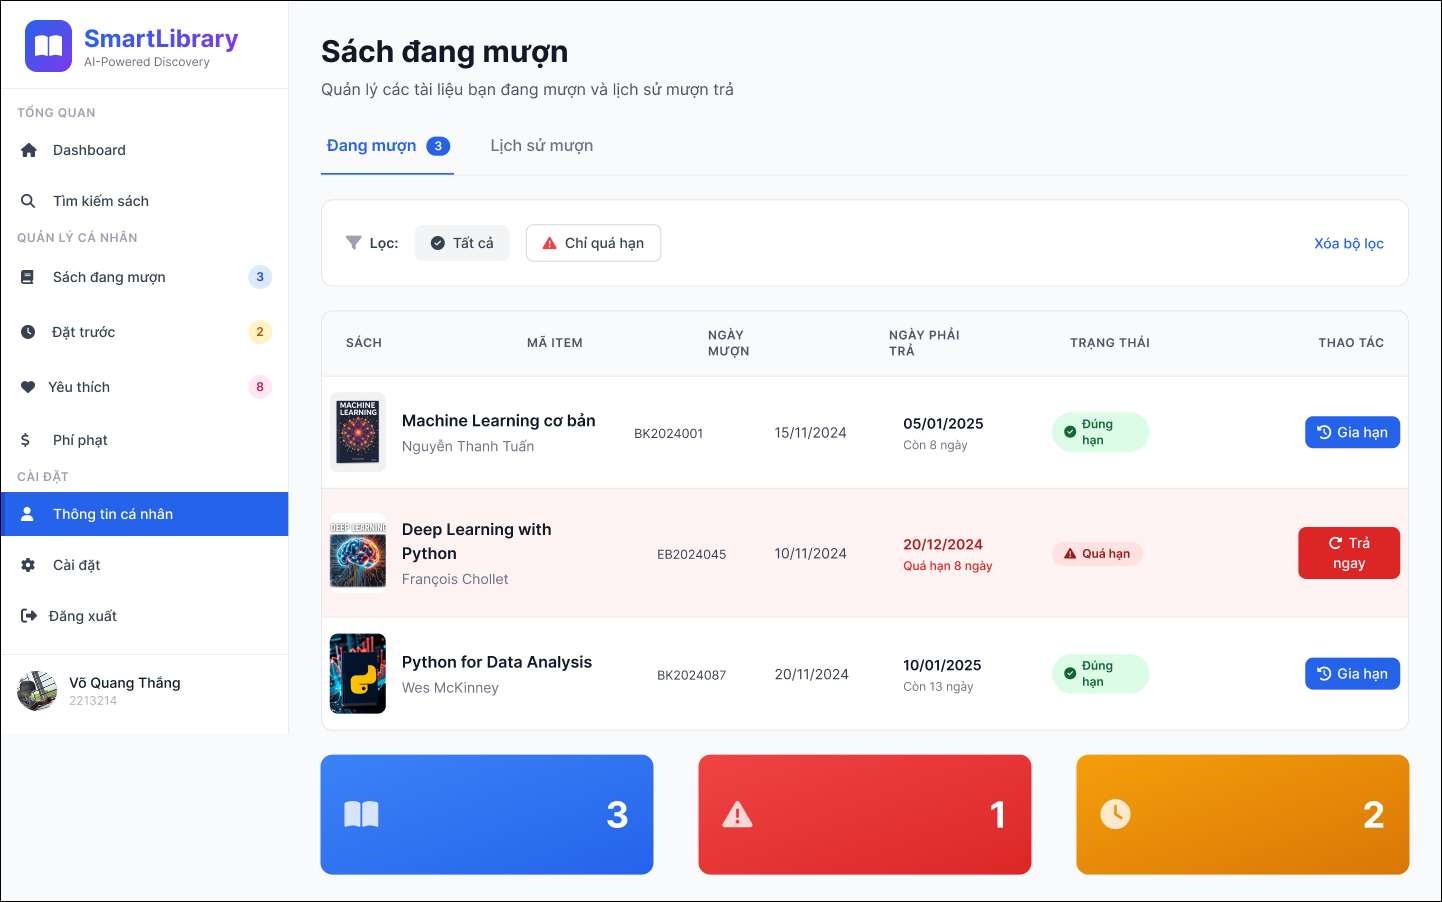
\includegraphics[width=\linewidth, height=0.38\textheight, keepaspectratio]{images/user_pages/sachdangmuon.png}
        \caption{Quản lý sách đang mượn}
        \label{fig:user_borrowing}
    \end{subfigure}
    \caption{Giao diện Độc giả: Dashboard và Quản lý mượn sách}
\end{figure}
\FloatBarrier

\subsubsection{Giao diện Thủ thư (Librarian Pages)}

\begin{figure}[htbp]
    \centering
    \begin{subfigure}[t]{0.48\linewidth}
        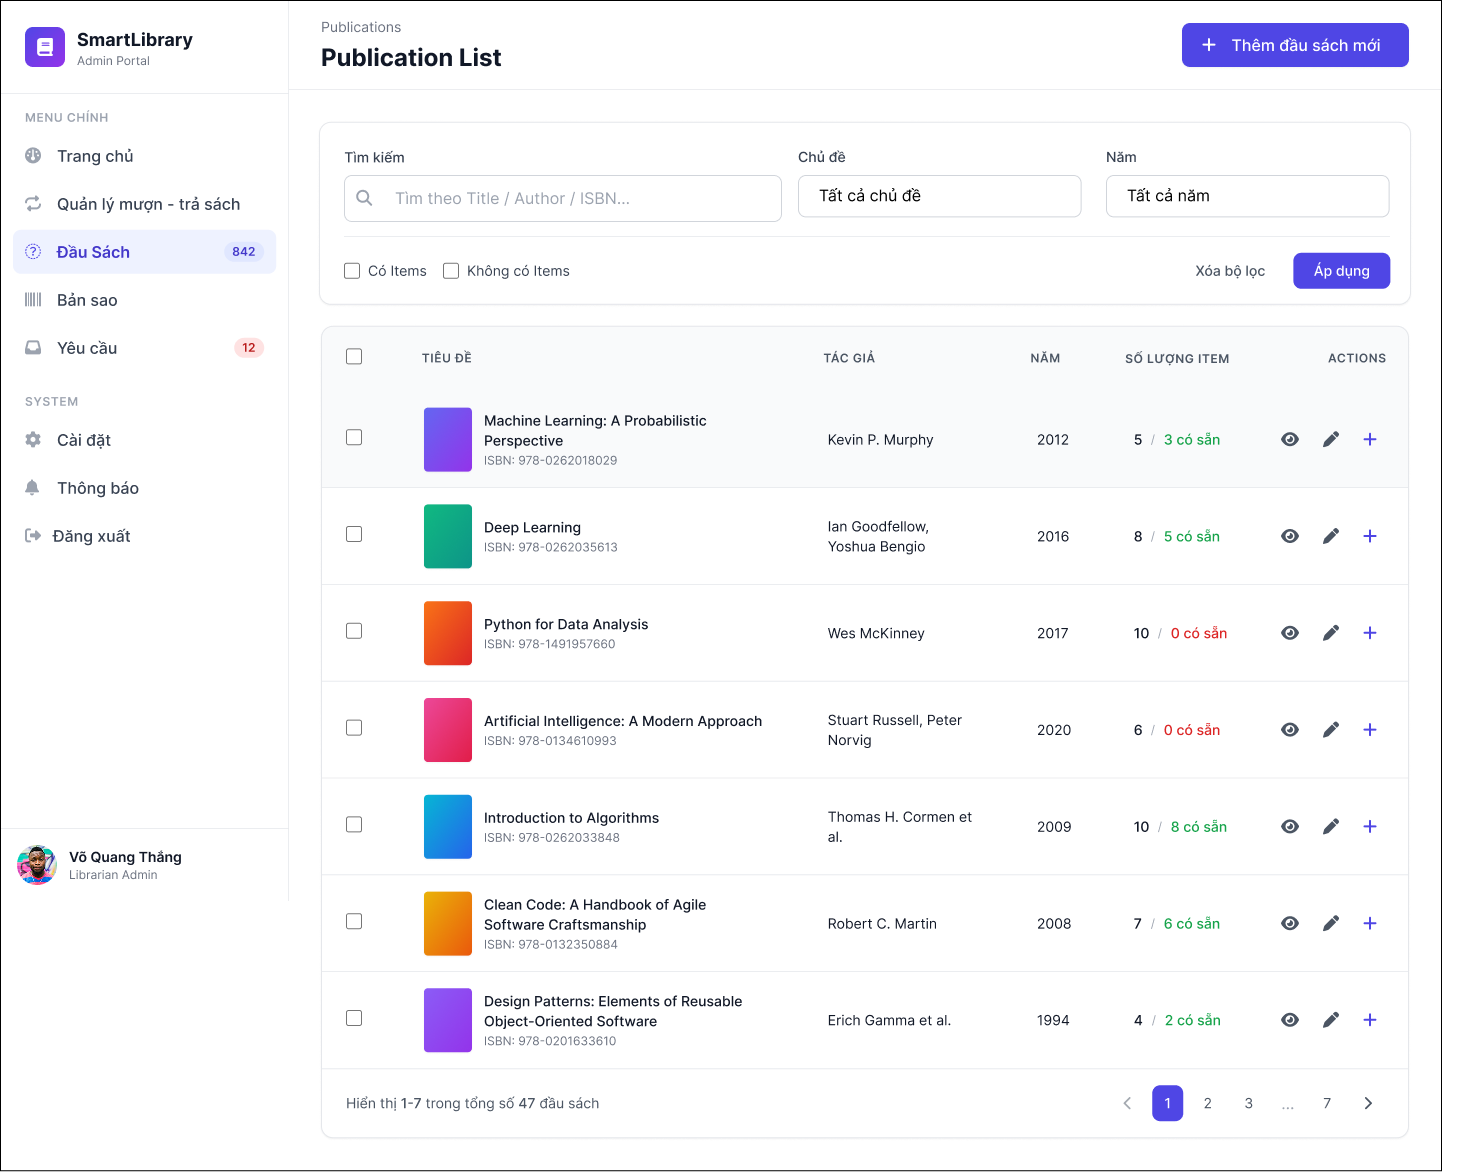
\includegraphics[width=\linewidth, height=0.38\textheight, keepaspectratio]{images/librarian_pages/Publishcation_list.png}
        \caption{Quản lý danh mục sách}
        \label{fig:lib_pub_list}
    \end{subfigure}
    \hfill
    \begin{subfigure}[t]{0.48\linewidth}
        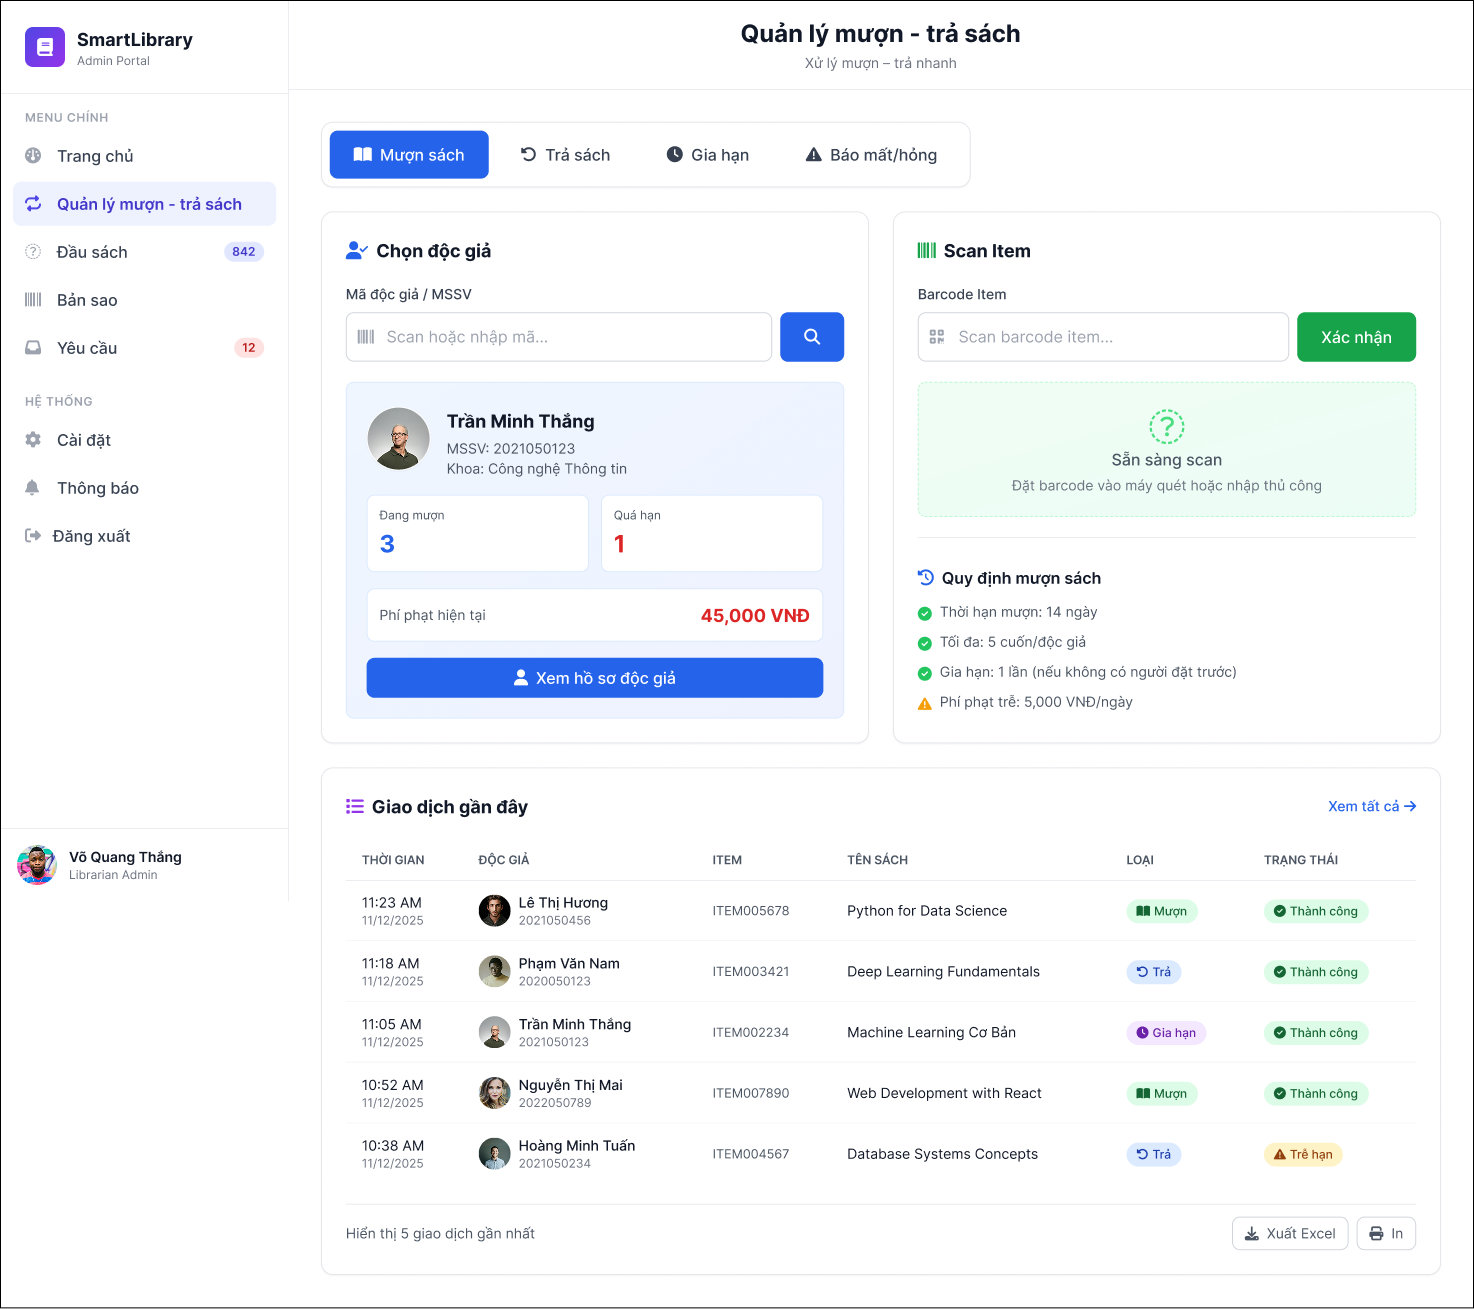
\includegraphics[width=\linewidth, height=0.38\textheight, keepaspectratio]{images/librarian_pages/muonsach.png}
        \caption{Ghi nhận mượn sách (Check-out)}
        \label{fig:lib_checkout}
    \end{subfigure}
    \caption{Giao diện Thủ thư: Quản lý danh mục và Lưu thông}
\end{figure}
\FloatBarrier